%\documentclass[10pt]{amsart}
%
%\usepackage{macros,slashed}
%
%\linespread{1.25}
%
%\usepackage{tikz,tikz-cd}
%\usetikzlibrary{arrows,shapes}
%\usetikzlibrary{trees}
%\usetikzlibrary{matrix,arrows}
%\usetikzlibrary{positioning}
%\usetikzlibrary{calc,through}
%\usetikzlibrary{decorations.pathreplacing}
%\usepackage{pgffor}
%
%\usetikzlibrary{decorations.pathmorphing}
%\usetikzlibrary{decorations.markings}
%\tikzset{
%	% >=stealth', %%  Uncomment for more conventional arrows
%    vector/.style={decorate, decoration={snake}, draw},
%	provector/.style={decorate, decoration={snake,amplitude=2.5pt}, draw},
%	antivector/.style={decorate, decoration={snake,amplitude=-2.5pt}, draw},
%    fermion/.style={draw=black, postaction={decorate},
%        decoration={markings,mark=at position .55 with {\arrow[draw=black]{>}}}},
%    fermionbar/.style={draw=black, postaction={decorate},
%        decoration={markings,mark=at position .55 with {\arrow[draw=black]{<}}}},
%    fermionnoarrow/.style={draw=black},
%    gluon/.style={decorate, draw=black,
%        decoration={coil,amplitude=4pt, segment length=5pt}},
%    scalar/.style={dashed,draw=black, postaction={decorate},
%        decoration={markings,mark=at position .55 with {\arrow[draw=black]{>}}}},
%    scalarbar/.style={dashed,draw=black, postaction={decorate},
%        dwecoration={markings,mark=at position .55 with {\arrow[draw=black]{<}}}},
%    scalarnoarrow/.style={dashed,draw=black},
%    electron/.style={draw=black, postaction={decorate},
%        decoration={markings,mark=at position .55 with {\arrow[draw=black]{>}}}},
%	bigvector/.style={decorate, decoration={snake,amplitude=4pt}, draw},
%}
%
%\usepackage[final]{pdfpages}
%
%\title{The higher dimensional holomorphic $\sigma$-model}
%
%\def\brian{\textcolor{blue}{BW: }\textcolor{blue}}
%
%\begin{document}
%\maketitle
%\tableofcontents

\chapter{The holomorphic $\sigma$-model}\label{chap: holsig}

This chapter contains a detailed analysis of one of the most fundamental holomorphic field theories: the holomorphic $\sigma$-model.
This theory is appealing from both the perspective of mathematics and physics.
It is an elegant nonlinear $\sigma$-model of maps complex $d$-fold $Y$ into a complex manifold $X$ (of any complex dimension). The equations of motion pick out the holomorphic maps. 
Thus, from a purely mathematical perspective, it is a compelling example to study 
because the classical theory naturally involves complex geometry and so must the quantization, although the meaning is less familiar. 

From a physical perspective, this class of theories is intimately related to supersymmetric field theories in various dimensions.
The most familiar supersymmetric $\sigma$-model is the two-dimensional $\cN=(2,2)$ theory which admits two topological twists, the $A$ and $B$-twists.
In two dimensions, the theory we consider arises naturally as a close cousin: it is a half-twist of the $\cN = (0,2)$, see for instance \cite{WittenCDO}.
The $\cN = (0,2)$ does {\em not} admit a twist that is topological, but does twist to a complex one-dimensional holomorphic theory more commonly referred to as the curved $\beta\gamma$ system.
In complex dimension two, we will see, in a similar vein, how the holomorphic $\sigma$-model arises as a twist of $\cN = 1$ supersymmetry in four real dimensions. 
There is a similar result in dimension six.
In a different direction, we show in \cite{GGW} that the holomoprhic $\sigma$-model is the chiral sector of the infinite volume limit of the usual (non-supersymmetric) $\sigma$-model. 
%In consequence, the curved $\beta\gamma$ system exhibits many features of these theories while enjoying the flavor of complex geometry, rather than super- or Riemannian geometry.

In complex dimension one, this theory has appeared in a hidden form in the work of Beilinson-Drinfeld and Malikov-Schechtman-Vaintrob \cite{BD,MSV}, and it was subsequently developed by many mathematicians (see \cite{KV,Cheung,Bressler} among much else). The {\em chiral differential operators} (CDOs) on a complex $n$-manifold $X$ are a sheaf of vertex algebras locally resembling a vertex algebra of $n$ free bosons, and the name indicates the analogy with the differential operators, a sheaf of associative algebras on $X$ locally resembling the Weyl algebra for $T^*\CC^n$. Unlike the situation for differential operators, which exist on any manifold $X$, such a sheaf of vertex algebras exists only if $\ch_2(X) = 0$ in $H^2(X, \Omega^2_{cl})$, and each choice of trivialization $\alpha$ of this characteristic class yields a different sheaf $\CDO_{X,\alpha}$. In other words, there is a gerbe of vertex algebras over $X$, \cite{GMS}. The appearance of this topological obstruction (essentially the first Pontryagin class, but non-integrally) was surprising, and even more surprising was that the character of this vertex algebra was the Witten genus of $X$, up to a constant depending only on the dimension of $X$ \cite{BorLib}. These results exhibited the now-familiar rich connections between conformal field theory, geometry, and topology, but arising from a mathematical process rather than a physical argument. 

Witten \cite{WittenCDO} explained how CDOs on $X$ arise as the perturbative piece of the chiral algebra of the curved $\beta\gamma$ system, by combining standard methods from physics and mathematics. (In elegant lectures on the curved $\beta\gamma$ system \cite{Nek}, with a view toward Berkovit's approach to the superstring, Nekrasov also explains this relationship.  Kapustin \cite{KapCDR} gave a similar treatment of the closely-related chiral de Rham complex.) This approach also gave a different understanding of the surprising connections with topology, in line with anomalies and elliptic genera as seen from physics. 
Let us emphasize that only the perturbative sector of the theory appears (i.e., one works near the constant maps from $\Sigma$ to $T^*X$, ignoring the nonconstant holomorphic maps); the instanton corrections are more subtle and not captured just by CDOs (see \cite{KapOrlov} for a treatment of the instanton corrections for complex tori).

In this paper we construct mathematically the perturbative sector of the holomorphic $\sigma$-model where the source is allowed to have arbitrary complex dimension.
We use the approach to quantum field theory developed in \cite{CostelloRenormalization, CG1,CG2}, thus providing a rigorous construction of the path integral for the holomorphic $\sigma$-model. That means we work in the homotopical framework for field theory known as the Batalin-Vilkovisky (BV) formalism, in conjunction with Feynman diagrams and renormalization methods. 
Just as CDO's have an anomaly we find that the higher dimensional theory admits a quantized action satisfying the quantum master equation only if the target manifold $X$ has $\ch_{d+1}(X) = 0$, where $\ch_{d+1}(X)$ is the $(d+1)$st component of the Chern character.

One key feature of the framework in \cite{CG2} is that every BV theory yields a factorization algebra of observables. (We mean here the version of factorization algebras developed in \cite{CG1}, not the version of Beilinson and Drinfeld \cite{BD}.)
In our situation, locally speaking the theory produces a factorization algebra living on the source manifold $\CC^d$.
When $d=1$ the machinery of \cite{CG1} allows one to extract a vertex algebra from this factorization algebra.
It is the main result of our work in \cite{GGW} that this vertex algebra is precisely the sheaf of CDOs.
One can interpret this as showing that in a wholly mathematical setting, one can start with the action functional for the curved $\beta\gamma$ system
and recover the sheaf $\CDO_{X,\alpha}$ of vertex algebras on $X$ via the algorithms of \cite{CostelloRenormalization, CG1, CG2}.
In higher dimensions we take the sheaf on $X$ of factorization algebras on $\CC^d$ produced via our work as a definition of higher dimensional chiral differential operators.
The higher dimensional theory of vertex algebras has not been fully developed, but we still show how to extract sensitive algebraic objects from this factorization algebras, such as an $A_\infty$-algebra which one can view as a deformation quantization of the mapping space ${\rm Map}(S^{2d-1}, X)$. 

Let us explain a little about our methods before stating our theorems precisely. 
The main technical challenge is to encode the nonlinear $\sigma$-model in a way so that the BV formalism of \cite{CostelloRenormalization} applies. 
In \cite{WG2}, Costello introduces a sophisticated approach by which he recovers the anomalies and the Witten genus as partition function, but it seems difficult to relate the local operators (e.g. CDO's in dimension one) directly to the factorization algebra of observables of his quantization. 
Instead, we use formal geometry {\it \`a la} Gelfand and Kazhdan \cite{GK}, as applied to the Poisson $\sigma$-model by Kontsevich \cite{KonDQ} and Cattaneo-Felder \cite{CF}.
The basic idea of Gelfand-Kazhdan formal geometry is that every $n$-manifold $X$ looks, very locally, like the formal $n$-disk, and so any representation $\sV$ of the formal vector fields and formal diffeomorphisms determines a vector bundle $\sV \to X$, by a sophisticated variant of the associated bundle construction. (Every tensor bundle arises in this way, for instance.) In particular, the Gelfand-Kazhdan version of characteristic classes for $\sV$ live in the Gelfand-Fuks cohomology $H^*_{\rm Lie}(\Vect)$ and map to the usual characteristic classes for $\sV$. There is, for instance, a Gelfand-Fuks version of the Witten class for every tensor bundle.

Thus, we start with the $\beta\gamma$ system on $\CC^d$ with target the formal $n$-disk $\widehat{D}^n = \rm{Spec}\,\CC[[t_1,\ldots,t_n]]$ and examine whether it quantizes \emph{equivariantly} with respect to the actions of formal vector fields $\Vect$ and formal diffeomorphisms on the formal $n$-disk.\footnote{In fact, we will see that it is enough to consider formal vector fields along with the finite dimensional Lie group of linear changes of frame $\GL_n$} (These actions are compatible, so that we have a representation of a Harish-Chandra pair.) We call this theory the \emph{equivariant formal $\beta\gamma$ system of rank $n$}.

\begin{thm}
The $\Vect$-equivariant formal $\beta\gamma$ system on $\CC^d$ of rank $n$ has a one-loop anomaly given by the cocycle $\ch_{d+1} (\widehat{D}^n)$ in the Gelfand-Fuks complex $\clie^*(\Vect ; \widehat{\Omega}^{d+1}_{n,cl})$. 
This cocycle determines an $L_\infty$ algebra extension $\TVectd$ of $\Vect$ and yields a $\TVectd$-equivariant BV quantization, unique up to homotopy. 
When $d=1$, the partition function of this theory over the moduli of elliptic curves is the formal Witten class in the Gelfand-Fuks complex $\clie^*(\Vect, \bigoplus_k \widehat{\Omega}_n^k[k])[[\hbar]]$.
\end{thm}

Throughout this paper, $\clie^*$ means the continuous Lie algebra cohomology, thus $\clie^*(\Vect, M)$ is the well-known cohomology studied by Gelfand and Fuks \cite{Fuks}. 

Gelfand-Kazhdan formal geometry is used often in deformation quantization. See, for instance, the elegant treatment by Bezrukavnikov-Kaledin \cite{BK}. Here we develop a version suitable for vertex algebras and factorization algebras, which requires allowing homotopical actions of the Lie algebra $\Vect$. (Something like this appears already in \cite{BD,KV,Malikov2008}, but we need a method with the flavor of differential geometry and compatible with Feynman diagrammatics. It would be interesting to relate directly these different approaches.) In consequence, our equivariant theorem implies the following global version.
 
 \begin{thm}
 \label{thm: holsig}
Let $d \geq 1$, and let $X$ be a complex manifold. 
The holomorphic $\sigma$-model of maps $\CC^d \to X$ admits a BV quantization if the class
\ben
\ch_{d+1} (T^{1,0}X) \in H^{d+1}(X ; \Omega^{d+1}_{cl}) \hookrightarrow H^{2d+2}_{dR}(X),
\een
vanishes.
Moreover, when this class vanishes the space of all quantizations is a torsor for the abelian group $H^d(X, \Omega^{d+1}_{cl})$. 
\end{thm}

When $d=1$ we showed in \cite{GGW} how the resulting factorization algebra produced by this result recovers CDO's. 
Further, when we place the theory on an elliptic curve we recover the Witten genus of the target manifold. 
In higher dimensions we provide a detailed analysis of the local operators in this theory that is similar in nature to the operators of a chiral CFT. 
Indeed, we show how the state space is a natural module for the operators on higher dimensional annuli (neighborhoods of spheres). 
A full theory of higher dimensional vertex algebras has not been fully developed. 
It is an interesting question to relate our higher dimensional holomorphic factorization algebras to the more algebro-geometric theory of higher dimensional chiral algebras as in Francis-Gaitsgory \cite{FrancisGaitsgory}. 

%We also show how our construction yields a quantization on source manifolds that have interesting topology. 
%We focus primarily on the case of Hopf manifolds, which are complex manifolds that are homeomorphic to $S^{2d-1} \times S^1$. 
%When the target is flat we compute the partition function and show that it agrees with the Witten index of the corresponding superconformal field theory. 
%In general the partition function of our quantization yields a complex invariant of the target manifold that varies holomorphically over the moduli of Hopf surfaces. 
%In future work we hope to relate this to a type of cohomology theory in a similar way that the Witten genus is related to elliptic cohomology and $tmf$. 

Our techniques for assembling BV theories in families --- and their factorization algebras in families --- apply to many $\sigma$-models already constructed , such as the topological $B$-model \cite{LiLi}, Rozansky-Witten theory \cite{CLL}, and topological quantum mechanics \cite{GG1, GLL}. 
They also allow us to recover quickly nearly all the usual variants on CDOs and structures therein, such as the chiral de Rham complex and the Virasoro actions.
In complex dimension one we recover the usual requirement that the target be Calabi-Yau.
One can also study the problem of quantizing a higher dimensional version of the Virasoro action, which we leave to a later publication. 
In general there is a more sensitive obstruction, which is still satisfied so long as the target admits a flat connection.

In the final section of this chapter we turn to a description of the local operators of the theory. 
The factorization algebra of observables is holomorphically translation invariant, in the sense of Section \ref{sec: hol trans}.
We show that there is a subspace of the operators supported on the sphere in $\CC^d$ that the factorization product endows with the structure of an associative algebra.
Further, we show that the state space is a natural dg module for this associative algebra, and we express it as a vacuum representation of the sphere algebra. 

\section{Gelfand-Kazhdan formal geometry} \label{sec: gk formal geometry}

In this section we review the theory of Gelfand-Kazhdan formal geometry and its use in natural constructions in differential geometry, organized in a manner somewhat different from the standard approaches.
We emphasize the role of the frame bundle and jet bundles.
We conclude with a treatment of the Atiyah class, which may be our only novel addition (although unsurprising) to the formalism.
We refer to our treatment of Harish-Chandra pairs and Harish-Chandra geometry given in Part I of \cite{GGW}.

We remark that from hereon we will work with complex manifolds and holomorphic vector bundles.
 
\subsection{A Harish-Chandra pair for the formal disk}

Let $\hO_n$ denote the algebra of formal power series 
\ben
\CC [[ t_1,\ldots,t_n ]],
\een 
which we view as ``functions on the formal $n$-disk $\hD^n$.'' 
It is filtered by powers of the maximal ideal $\fm_n = (t_1,\ldots,t_n)$, and it is the limit of the sequence of artinian algebras
\[
\cdots \to \hO_n/(t_1,\ldots,t_n)^k \to \cdots \hO_n/(t_1,\ldots,t_n)^2 \to \hO_n/(t_1,\ldots,t_n) \cong \CC.
\] 
We equip $\hO_n$ and its modules with the associated adic topology.

We use $\Vect$ to denote the Lie algebra of derivations of $\hO_n$, which consists of first-order differential operators with formal power series coefficients:
\[
\Vect = \left\{ \sum_{i =1 }^n f_i \frac{\partial}{\partial t_i} \,:\, f_i \in \hO_n\right\}.
\]
The group $\GL_n$ also acts naturally on $\hO_n$: for $M \in \GL_n$ and $f \in \hO_n$,
\[
(M \cdot f)(t) = f (Mt),
\]
where on the right side we view $t$ as an element of $\CC^n$ and let $M$ act linearly.
In other words, we interpret $\GL_n$ as acting ``by diffeomorphisms'' on $\hD^n$ and then use the induced pullback action on functions on $\hD^n$.
The actions of both $\Vect$ and $\GL_n$ intertwine with multiplication of power series, 
since ``the pullback of a product of functions equals the product of the pullbacks.''

\subsubsection{Formal automorphisms}

Let $\Aut_n$ be the group of filtration-preserving automorphisms of the algebra $\hO_n$,
which we will see is a pro-algebraic group.
Explicitly, such an automorphism $\phi$ is a map of algebras that preserves the maximal ideal, 
so $\phi$ is specified by where it sends the generators $t_1$, \dots, $t_n$ of the algebra.
In other words, each $\phi \in \Aut_n$ consists of an $n$-tuple $(\phi_1,\ldots,\phi_n)$ 
such that each $\phi_i$ is in the maximal ideal generated by $(t_1,\ldots,t_n)$ and such that there exists an $n$-tuple $(\psi_1,\ldots,\psi_n)$ 
where the composite
\[
\psi_j(\phi_1(t),\ldots,\phi_n(t)) = t_j
\]
for every $j$ (and likewise with $\psi$ and $\phi$ reversed).
This second condition can be replaced by verifying that the Jacobian matrix
\[
Jac(\phi) = (\partial \phi_i/\partial t_j) \in {\rm Mat}_n(\hO_n)
\]
is invertible over $\hO_n$, by a version of the inverse function theorem.

Note that this group is far from being finite-dimensional, so it does not fit immediately into the setting of Harish-Chandra pairs described above. 
It is, however, a {\em pro}-Lie group in the following way. 
As each $\phi \in \Aut_n$ preserves the filtration on $\hO_n$, it induces an automorphism of each partial quotient $\hO_n/\fm_n^k$.
Let $\Aut_{n,k}$ denote the image of $\Aut_n$ in $\Aut(\hO_n/\fm_n^k)$; this group $\Aut_{n,k}$ is clearly a quotient of $\Aut_n$.
Note, for instance, that $\Aut_{n,1} = \GL_n$.
Explicitly, an element $\phi$ of ${\rm Aut}_{n,k}$ is the collection of $n$-tuples $(\phi_1,\ldots,\phi_n)$ 
such that each $\phi_i$ is an element of $\fm_n/\fm_n^k$ and such that the Jacobian matrix $Jac(\phi)$ is invertible in $\hO_n/\fm_n^k$.
The group ${\rm Aut}_{n,k}$ is manifestly a finite dimensional Lie group, as the quotient algebra is a finite-dimensional vector space. 
 
The group of automorphisms $\Aut_n$ is the pro-Lie group associated with the natural sequence of Lie groups
\ben
\cdots \to \Aut_{n,k} \to \Aut_{n,k-1} \to \cdots \to \Aut_{n,1} = \GL_n.
\een
Let $\Aut_n^+$ denote the kernel of the map $\Aut_n \to \GL_n$ so that we have a short exact sequence
\ben
1 \to \Aut_n^+ \to \Aut_n \to \GL_n \to 1 .
\een
In other words, for an element $\phi$ of $\Aut_n^+$, each component
$\phi_i$ is of the form $t_i + \cO(t^2)$. The group $\Aut_n^+$ is
pro-nilpotent, hence contractible. 

The Lie algebra of $\Aut_n$ is {\em not} the Lie algebra of formal
vector fields $\Vect$. A direct
calculation shows that the Lie algebra of $\Aut_n$ is the Lie algebra $\Vectz \subset \Vect$ of formal vector fields with zero constant coefficient (i.e., that vanish at the origin of $\hD^n$). 

Observe that the group $\GL_n$ acts on the Lie algebra $\Vect$ by the obvious linear ``changes of frame.''
The Lie algebra $\Lie({\GL_n}) = \fgl_n$ sits inside $\Vect$ as the linear vector fields
\ben
\left\{\sum_{i,j} a^j_i t_i \frac{\partial}{\partial t_j} \; : \; a^{i}_j \in \CC \right\}.
\een 
We record these compatibilities in the following statement.

\begin{lem} 
The pair $(\Vect, \GL_n)$ form a Harish-Chandra pair.
\end{lem}
\begin{proof} The only thing to check is that the derivative of the
  action of $\GL_n$ corresponds with the adjoint action of $\fgl_n
  \subset \Vect$ on formal vector fields. This is by construction. 
\end{proof}

\subsection{Formal coordinates}

In this section we review the central object in the Gelfand-Kazhdan
picture of formal geometry: the coordinate bundle.

%Our version of Harish-Chandra localization is intimately related to, and motivated by, the methods of formal geometry developed by Gelfand, Fuchs, Kazhdan, and many others \brian{refs}. 
%It has been used prominently in the setting of deformation quantization, notably by Kontsevich \brian{ref}, Nest-Tsygan \brian{ref}, Cattaneo-Felder \brian{ref}, and \brian{more}. 
%Here we start by reviewing the big picture before delving into some precise definitions and summarizing the relevant results from the literature.

\subsubsection{The coordinate bundle}

Given a complex manifold, its {\em coordinate space} $X^{coor}$ is the (infinite-dimensional) space parametrizing jets of holomorphic coordinates of $X$. 
(It is a pro-complex manifold, as we'll see.) 
Explicitly, a point in $X^{coor}$ consists of a point $x \in X$ 
together with an $\infty$-jet class of a local biholomorphism $\phi : U \subset \CC^n \to X$ 
sending a neighborhood $U$ of the origin to a neighborhood of $x$ such that $\phi(0) = x$. 

There is a canonical projection map $\pi^{coor} : X^{coor} \to X$ by remembering only the underlying point in $X$. 
The group $\Aut_n$ acts on $X^{coor}$ by ``change of coordinates," 
i.e., by precomposing a local biholomorphism $\phi$ with an automorphism of the disk around the origin in $\CC^n$.
This action identifies $\pi^{coor}$ as a principal bundle for the pro-Lie group $\Aut_n$. 

One way to formalize these ideas is to realize $X^{coor}$ as a limit of finite-dimensional complex manifolds. 
Let $X_k^{coor}$ be the space consisting of points $(x, [\phi]_k)$, 
where $\phi$ is a local biholomorphism as above and $[-]_k$ denotes taking its $k$-jet equivalence class. 
Let $\pi_k^{coor} : X^{coor}_k \to X$ be the projection. 
By construction, the finite-dimensional Lie group $\Aut_{n,k}$ acts on the fibers of the projection freely and transitively 
so that $\pi_k^{coor}$ is a principal $\Aut_{n,k}$-bundle. The bundle $X^{coor} \to X$ is the limit of the sequence of principal bundles on X
\ben
\xymatrix{
\cdots \ar[r] & X^{coor}_k \ar[r] \ar[drrrr]_-{\pi_k^{coor}} & X^{coor}_{k-1} \ar[drrr]^-{\pi_{k-1}^{coor}} \ar[r] & \cdots \ar[r] & X_2^{coor} \ar[dr]^{\pi_2^{coor}} \ar[r] & X_1^{coor} \ar[d]^-{\pi_1^{coor}} \\ 
 & & & & & X .
}
\een

In particular, note that the $\GL_n = \Aut_{n,1}$-bundle $\pi_1^{coor} : X^{coor}_1 \to X$ is the frame bundle
\ben
\pi^{fr} : {\rm Fr}_X \to X,
\een
i.e., the principal bundle associated to the tangent bundle of $X$.

\subsubsection{The Grothendieck connection} 

We can also realize the Lie algebra $\Vect$ as an inverse limit. 
Recall the filtration on $\Vect$ by powers of the maximal ideal $\fm_n$ of $\hO_n$. 
Let ${\rm W}_{n,k}$ denote the quotient $\Vect / \fm_n^{k+1} \Vect$. 
For instance, ${\rm W}_{n,1} = \mathfrak{aff}_n = \CC^n \ltimes \fgl_n$, the Lie algebra of affine transformations of $\CC^n$. We have $\Vect = \lim_{k \to \infty} {\rm W}_{n,k}$. 

The Lie algebra of $\Aut_{n,k}$ is
\[
{\rm W}_{n,k}^0 := \fm_n \cdot \Vect /\fm_n^{k+1} \Vectz .
\]
That is, the Lie algebra of vector fields vanishing at zero modulo the $k+1$ power of the maximal ideal. Thus, the principal $\Aut_{n,k}$-bundle $X_{k}^{coor} \to X$ induces an exact sequence of tangent spaces
\ben
{\rm W}_{n,k}^0 \to T_{(x,[\varphi]_k)}X^{coor} \to T_x X;
\een
by using $\varphi$, we obtain a canonical isomorphism of tangent spaces $\CC^n \cong T_0 \CC^n \cong T_x X$. Combining these observations, we obtain an isomorphism
\ben
{\rm W}_{n,k} \cong T_{(x,[\varphi]_k)} X^{coor}_k .
\een
In the limit $k \to \infty$ we obtain an isomorphism $\Vect \cong T_{(x,[\varphi]_\infty)} X^{coor}$. 

\begin{prop}[Section 5 of \cite{NT}, Section 3 of \cite{CF2}]
There exists a canonical action of $\Vect$ on $X^{coor}$ by
holomorphic vector fields, i.e., there is a Lie algebra homomorphism
\ben
\theta : \Vect \to \cX^{hol}(X^{coor}) ,
\een
where $\cX^{hol}(X^{coor})$ is the Lie algebra of holomorphic vector fields.
Moreover, this action induces the isomorphism $\Vect \cong
T_{(x,[\phi]_\infty)} X^{coor}$ at each point.
\end{prop}

\noindent Here, $\cX(X^{coor})$ is understood as the inverse limit of the finite-dimensional Lie algebras $\cX(X^{coor}_k)$.

The inverse of the map $\theta$ provides a connection one-form
\ben
\omega^{coor} \in \Omega^1_{hol}(X^{coor}; \Vect),
\een
which we call the {\em universal Grothendieck connection} on $X$. 
As $\theta$ is a Lie algebra homomorphism, $\omega^{coor}$ satisfies the Maurer-Cartan equation
\be\label{mc}
\partial \omega^{coor} + \frac{1}{2} [\omega^{coor},\omega^{coor}] = 0 .
\ee
Note that the proposition ensures that this connection is universal on all complex manifolds of dimension $n$ 
and indeed pulls back along local biholomorphisms.

\begin{rmk}
We can view $\omega^{coor}$ as an element of the full de Rham complex $\omega^{coor} \in \Omega^1(X^{coor} ; \Vect)$ where the Maurer-Cartan equation reads $\d \omega + \frac{1}{2} [\omega^{coor}, \omega^{coor}] = 0$.
\end{rmk}

\begin{rmk} 
Both the pair $(\Vect, \Aut)$ and the bundle $X^{coor} \to X$ together
with $\omega^{coor}$ do not fit in the finite dimensional models for
Harish-Chandra geometry.
They are, however, objects in a larger category of pro-Harish-Chandra pairs and pro-Harish-Chandra bundles, respectively. 
We do not fully develop this theory here, but it is inherent in the work of
\cite{BK}.  
Indeed, by working with well-behaved representations for the pair $(\Vect,\Aut)$, 
Gelfand, Kazhdan, and others use this universal construction to produce many of the natural constructions in differential geometry.
As we remarked earlier, it is a kind of refinement of tensor calculus.
\end{rmk}

\subsubsection{A Harish-Chandra structure on the frame bundle}

\def\Sect{{\rm Sect}}
\def\Fr{{\rm Fr}}
\def\Exp{{\rm Exp}}

Although the existence of the coordinate bundle
$X^{coor}$ is necessary in the remainder of this paper, it is convenient for us to use it in a rather
indirect way. Rather, we will work with the frame bundle ${\rm Fr}_X \to X$ equipped with the structure of a module for the Harish-Chandra pair $(\Vect, \GL_n)$. 
The $\Vect$-valued connection on $\Fr_X$ is induced from the Grothendieck connection above.

\begin{dfn}\label{fmlexp} 
Let $\Exp (X)$ denote the quotient $X^{coor} / \GL_n$. 
A holomorphic section of $\Exp(X)$ over $X$ is called a {\em formal exponential}. 
\end{dfn}

\begin{rmk} 
The space $\Exp(X)$ can be equipped with the structure of a principal $\Aut_n^+$-bundle over $X$.
This structure on $\Exp(X)$ depends on a choice of a section of the short exact sequence
\ben
1 \to \Aut_n^+ \to \Aut_n \to \GL_n \to 1 .
\een
It is natural to use the splitting determined by the choice of coordinates on the formal disk.
\end{rmk}

Note that $\Aut_n^+$ is contractible, and so sections always exist. 
A formal exponential is useful because it equips the frame bundle with a $(\Vect,\GL_n)$-module structure, as follows.

%The space of formal exponentials is the (infinite dimensional) affine space $\Sect_X(\Exp_X^\infty)$. Unraveling the definition, such a section $\sigma$ of $X^{aff}$ is an $\infty$-jet equivalence class of a local diffeomorphism
%\ben
%\sigma_x : T_x X \to X
%\een
%for each $x \in X$ such that
%\begin{itemize}
%\item[(i)] $\sigma_x(0) = x$
%\item[(ii)]\label{exp2} The derivative at $0$ of $\sigma_x$ is the identity $D (\sigma)_0 = {\rm id} : T_x X \to T_x X$. 
%\end{itemize}
% 
%\begin{rmk} In \brian{Cattaneo-Felder, more} this bundle is denoted $X^{aff} \to X$ and is called the affine bundle. 
%\end{rmk}

\begin{prop} \label{gauge equiv} 
A formal exponential $\sigma$ pulls back to a $\GL_n$-equivariant map $\tilde{\sigma} : \Fr_X \to X^{coor}$,
and hence equips $(\Fr_x, \sigma^* \omega^{coor})$ with the structure
of a principal $(\Vect,\GL_n)$-bundle with flat connection.
Moreover, any two choices of formal exponential determine $(\Vect,\GL_n)$-structures on $X$ that are gauge-equivalent. 
\end{prop}

For a full proof, see \cite{NT}, \cite{nest1995}, or \cite{khors} but the basic idea is easy to explain.

\begin{proof}[Sketch of proof]
The first assertion is tautological, since the data of a section is equivalent to such an equivariant map, but we explicate the underlying geometry.
A map $\rho : \Fr_X \to X^{coor}$ assigns to each pair  $(x, \mathbf{y}) \in \Fr_X$,
with $x \in X$ and $\mathbf{y} : \CC^n \xto{\cong} T_x X$ a linear frame,
an $\infty$-jet of a biholomorphism $\phi: \CC^n \to X$ such that $\phi(0) = x$ and $D\phi(0) = \mathbf{y}$.
Being $\GL_n$-equivariant ensures that these biholomorphisms are related by linear changes of coordinates on $\CC^n$.
In other words, a $\GL_n$-equivariant map $\tilde{\sigma}$ describes how each frame on $T_x X$ exponentiates to a formal coordinate system around $x$,
and so the associated section $\sigma$ assigns a formal exponential map $\sigma(x) \colon T_x X \to X$ to each point $x$ in $X$.
(Here we see the origin of the name ``formal exponential.'')

The second assertion would be immediate if $X^{coor}$ were a complex manifold, since the flat bundle structure would pull back,
so all issues are about carefully working with pro-manifolds.

The final assertion is also straightforward: the space of sections is contractible since $\Aut_n^+$ is contractible, 
so one can produce an explicit gauge equivalence.
\end{proof}

% \owen{Explain that a connection on the tangent bundle produces local exponential maps and hence a formal exponential,
% an observation that Willwacher refines.}

% In practice, formal exponentials are easy to produce. Consider a connection on the holomorphic tangent bundle. \brian{finish this}

\begin{rmk} 
In \cite{willwacher} Willwacher provides a description of the space $\Exp(X)$ of {\em all} formal exponentials. He shows that it is isomorphic to the space of pairs $(\nabla_0, \Phi)$
where $\nabla_0$ is a torsion-free connection on $X$ for $T_X$ and $\Phi$ is a section of the bundle
\ben
\Fr_X \times_{\GL_n} {\rm W}_n^3
\een
where ${\rm W}_n^3 \subset \Vect$ is the subspace of formal vector fields whose coefficients are at least cubic. 
In particular, every torsion-free affine connection determines a formal exponential. The familiar case above that produces a formal coordinate from a connection corresponds to choosing the zero vector field. 
\end{rmk}

%Given a formal exponential $\sigma$ we now construct a formal vector field valued connection one-form $\omega_\sigma \in \Omega^1(\Fr_X; \Vect)$ satisfying the Maurer-Cartan equation. Hence, a $(\Vect,\GL_n)$-structure on $\Fr_X$. 
%
%Let $(x, \mathbf{y}) \in \Fr_X$. Define $\omega_\sigma_{(x, \mathbf{y})} : T_{(x, \mathbf{y})} \Fr_X \to \Vect$
%as the composition 
%\ben
%\xymatrix{
%T_{(x, \mathbf{y})} \Fr_X \ar[r]^-{D \sigma} & T_{(x, \sigma(\mathbf{y}))} X^{coor} \ar[r]^-{\omega^{coor}} & \Vect .
%}
%\een 
%This defines $\omega_\sigma \in \Omega^1(\Fr_X; \Vect)$. The fact that $\omega_\sigma$ is $\GL_n$-invariant follows from the fact that $D \sigma|_0$ is the identity. 
%
%\brian{MC equation, gauge equivalence for different choices of splitting}

\begin{dfn}
A {\em Gelfand-Kazhdan structure} is a complex manifold $X$ of dimension $n$ together with a formal exponential $\sigma$, 
which makes the frame bundle $\Fr_X$ into a flat $(\Vect,\GL_n)$-bundle with connection one-form $\omega_\sigma$, 
the pullback of $\omega^{coor}$ along the $\GL_n$-equivariant lift $\tilde{\sigma} : \Fr_X \to X^{coor}$.
\end{dfn}

\begin{eg} 
Consider the case of an open subset $U \subset \CC^n$. 
There are thus natural holomorphic coordinates $\{z_1,\ldots,z_n\}$ on $U$. 
These coordinates provides a natural choice of a formal exponential. 
Moreover, with respect to the isomorphism
\ben
\Omega^1_{hol}(\Fr_U ; \Vect)^{\GL_n} \cong \Omega^1_{hol}(U ; \Vect) \cong \sO^{hol}(U) [\d z_i] \tensor \Vect ,
\een
we find that the connection 1-form has the form
\ben
\omega^{coor} = \sum_{i=1}^n \d z_i \tensor \frac{\partial}{\partial t_i},
\een 
where the $\{t_i\}$ are the coordinates on the formal disk $\hD^n$.
\end{eg} 

A Gelfand-Kazhdan structure allows us to apply a version of Harish-Chandra descent, which will be a central tool in our work.

Although we developed Harish-Chandra descent on all flat $(\fg,K)$-bundles, 
it is natural here to restrict our attention to manifolds of the same dimension,
as the notions of coordinate and affine bundle are dimension-dependent.
Hence we replace the underlying category of all complex manifolds by a more restrictive setting.

\begin{dfn}
Let $\Hol_n$ denote the category whose objects are complex manifolds of dimension $n$ and whose morphisms are local biholomorphisms.
In other words, a map $f: X \to Y$ in $\Hol_n$ is a map of complex manifolds such that each point $x \in X$ admits a neighborhood $U$ on which $f|_U$ is biholomorphic with $f(U)$.
\end{dfn}

There is a natural inclusion functor $i : \Hol_n \to {\rm CplxMan}$ (not fully faithful) and the frame bundle $\Fr$ defines a section of the fibered category $i^*\VB$,
since the frame bundle pulls back along local biholomorphisms.
For similar reasons, the coordinate bundle is a pro-object in $i^*\VB$.

\begin{dfn}
Let $\GK_n$ denote the category fibered over $\Hol_n$ whose objects are a Gelfand-Kazhdan structure 
--- that is, a pair $(X, \sigma)$ of a complex $n$-manifold and a formal exponential ---
and whose morphisms are simply local biholomorphisms between the underlying manifolds.
\end{dfn}

Note that the projection functor from $\GK_n$ to $\Hol_n$ is an equivalence of categories, since the space of formal exponentials is affine.

\subsection{The category of formal vector bundles}

For most of our purposes, it is convenient and sufficient to work with a small category of $(\Vect,\GL_n)$-modules 
that is manifestly well-behaved and whose localizations appear throughout geometry in other guises, 
notably as $\infty$-jet bundles of vector bundles on complex manifolds.
(Although it would undoubtedly be useful, we will not develop here the general theory of modules for the Harish-Chandra pair $(\Vect,\GL_n)$, 
which would involve subtleties of pro-Lie algebras and their representations.)

We first start by describing the category of $(\Vect, \GL_n)$-modules
that correspond to modules over the structure sheaf of a manifold. Note that $\hO_n$ is the quintessential example of a commutative algebra object in the symmetric monoidal category of $(\Vect,\GL_n)$-modules, 
for any natural version of such a category. We consider modules that
have actions of both the pair and the algebra $\hO_n$ with obvious
compatibility restrictions. 

\begin{dfn} A {\em formal $\hO_n$-module} is a
  vector space $\cV$ equipped with
\begin{itemize}
\item[(i)] the structure of a $(\Vect, \GL_n)$-module;
\item[(ii)] the structure of a $\hO_n$-module;
\end{itemize}
such that 
\begin{itemize}
\item[(1)] for all $X \in \Vect$, $f \in \hO_n$ and $v \in \cV$ we
  have $X(f \cdot v) = X(f) \cdot v + f \cdot (X \cdot v)$;
\item[(2)] for all $A \in \GL_n$ we have $A (f \cdot v) = (A \cdot f) \cdot (A \cdot v)$,  where $A$ acts on $f$ by a linear change of frame.
\end{itemize}
A morphism of formal $\hO_n$-modules is a $\hO_n$-linear map of
$(\Vect, \GL_n)$-modules $f : \cV \to \cV'$. We denote this category
by $\Mod_{(\Vect, \GL_n)}^{\hO_n}$. 
\end{dfn}

Just as the category of $D$-modules is symmetric monoidal via tensor over $\hO$, we have the following result.

\begin{lem}
The category $\Mod^{\hO_n}_{(\Vect, \GL_n)}$ is symmetric monoidal with respect to tensor over $\hO_n$.
\end{lem} 

\begin{proof}
The category of $\hO_n$-modules is clearly symmetric monoidal by tensoring over $\hO_n$. We simply need to verify that the Harish-Chandra module structures extend in a natural way, but this is clear.
\end{proof}

We will often restrict ourselves to considering Harish-Chandra modules as above that are free as underlying $\hO_n$-modules. 
Indeed, let
\ben
\VB_n \subset \Mod_{(\Vect, \GL_n)}^{\hO_n}
\een
be the full subcategory spanned by objects that are free and finitely generated as underlying $\hO_n$-modules. 
Upon descent these will correspond to ordinary vector bundles and so
we refer to this category as {\em formal vector bundles}. 

The category of formal $\hO_n$-modules has a natural symmetric monoidal structure by tensor product over $\hO$. The Harish-Chandra action is extended by
\[
X \cdot (s \otimes t) = (X s) \otimes t + s \otimes (Xt). 
\]
This should not look surprising; it is the same formula for tensoring
$D$-modules over $\hO$. 

The internal hom $\Hom_{\hO}(\cV,\cW)$ also provides a vector bundle on the formal disk, 
where the Harish-Chandra action is extended by
\[
(X \cdot \phi)(v) = X \cdot (\phi(v)) - \phi(X\cdot v). 
\]

Observe that for any $D$-module $M$, we have an isomorphism
\[
\Hom_{D}(\hO, M) \cong \Hom_{\Vect}(\CC, M)
\]
since a map of $\hD$-modules out of $\hO$ is determined by where it sends the constant function 1. 
Hence we find that there is a quasi-isomorphism 
\[
\RR\Hom_{D}(\hO, \cV) \simeq \clie^*(\Vect ; \cV),
\]
or more accurately a zig-zag of quasi-isomorphisms. Here
$\clie^*(\Vect ; \cV)$ is the continuous cohomology of $\Vect$ with
coefficients in $\cV$. This is known as the {\em Gelfand-Fuks}
cohomology of $\cV$ and is what we use for the remainder of the
paper. 

This relationship extends to the $\GL_n$-equivariant setting as well, giving us the following result.

\begin{lem}
There is a quasi-isomorphism
\[
\clie^*(\Vect,\GL_n; \cV) \simeq \RR \Hom_D(\hO,\cV)^{\GL_n-{\rm eq}},
\]
where the superscript $\GL_n-{\rm eq}$ denotes the $\GL_n$-equivariant maps.
\end{lem}

\begin{rmk}
One amusing way to understand this category is as Harish-Chandra descent to the formal $n$-disk itself. 
Consider the frame bundle $\widehat{\Fr} = \hD^n \times \GL_n \to \hD^n$ of the formal $n$-disk itself, 
which possesses a natural flat connection via the Maurer-Cartan form $\omega_{MC}$ on $\GL_n$. 
Let $\rho: \GL_n \to \GL(V)$ be a finite-dimensional representation. 
Then the subcomplex of $\Omega^*(\widehat{\Fr})\otimes V$ given by the basic forms is isomorphic to
\[
\left(\Omega^*(\hD^n) \otimes V, \d_{dR} + \rho(\omega_{MC}) \right).
\]
This equips the associated bundle $\widehat{\Fr}\times^{\GL_n} V$ with a flat connection and 
hence makes its sheaf of sections a $D$-module on the formal disk.
\end{rmk}

Many of the important $\hO_n$-modules we will consider simply come from linear tensor representations of $\GL_n$. 
Given a finite-dimensional $\GL_n$-representation $V$, we construct a $\hO_n$-module $\cV \in \VB_n$ as follows. 

Consider the decreasing filtration of $\Vect$ by vanishing order of jets 
\ben
\cdots \subset \fm^{2}_n \cdot {\rm W}_{n} \subset \fm^1_n \cdot {\rm W}_n \subset {\rm W}_n .
\een 
The induced map $\fm_n^1 \cdot \Vect \to \fm_n^1 \cdot \Vect / \fm_n^2
\cdot \Vect \cong \fgl_n$ allows us to restrict $V$ to a $\fm_n^1 \cdot
\Vect$-module. 
We  then coinduce this module along the inclusion $\fm^1 \cdot \Vect
\subset \Vect$ to get a $\Vect$-module $\cV = \Hom_{\fm_n^1 \cdot \Vect}(\Vect,V)$. 
There is an induced action of $\GL_n$ on $\cV$. Indeed, as a $\GL_n$-representation one has $\cV \cong \hO_n \tensor_{\CC} V$.
Moreover, this action is compatible with the $\Vect$-module structure, so that $\cV$ is actually a $(\Vect, \GL_n)$-module. 
Thus, the construction provides a functor  from $\Rep_{\GL_n}$ to
$\VB_n$.

\begin{dfn} 
We denote by ${\rm Tens}_n$ the image of finite-dimensional $\GL_n$-representations in $\VB_n$ along this functor. 
We call it the category of {\em formal tensor fields}.
\end{dfn}

As mentioned $\hO_n$ is an example, associated to the trivial one-dimensional $\GL_n$ representation.
Another key example is $\hT_n$, the vector fields on the formal disk, which is associated to the defining $\GL_n$ representation $\CC^n$; 
it is simply the adjoint representation of $\Vect$.
Other examples include $\hOmega^1_n$, the 1-forms on the formal disk; it
is the correct version of the coadjoint representation, and more
generally the space of $k$-forms on the formal disk $\hOmega^k_n$. 

The category ${\rm Tens}_n$ can be interpreted in two other ways, as we will see in subsequent work.
\begin{enumerate}
\item They are the $\infty$-jet bundles of tensor bundles: for a finite-dimensional $\GL_n$-representation, 
construct its associated vector bundle along the frame bundle and take its $\infty$-jets.
\item They are the flat vector bundles of finite-rank on the formal $n$-disk that are equivariant with respect to automorphisms of the disk. 
In other words, they are $\GL_n$-equivariant $D$-modules whose underlying $\hO$-module is finite-rank and free.
\end{enumerate}
It should be no surprise that given a Gelfand-Kazhdan structure on the frame bundle of a non-formal $n$-manifold $X$, 
a formal tensor field descends to the $\infty$-jet bundle of the corresponding tensor bundle on $X$. 
The flat connection on this descent bundle is, of course, the Grothendieck connection on this $\infty$-jet bundle. 
(For some discussion, see section 1.3, pages 12-14, of \cite{Fuks}.)

Note that the subcategories 
\ben
{\rm Tens}_n \hookrightarrow \VB_n
\hookrightarrow \Mod_{(\Vect, \GL_n)}^{\hO_n}
\een
inherit the symmetric monoidal structure constructed above. 

\subsection{Gelfand-Kazhdan descent}

We will focus on defining descent for the category $\VB_n$ of formal vector
bundles. 

Fix an $n$-dimensional manifold $X$.
The main result of this section is that the associated bundle construction along the frame bundle $\Fr_X$,
\[
\begin{array}{cccc}
\Fr_X \times^{\GL_n} (-) :&  \Rep(\GL_n)^{fin} & \to &\VB(X)\\
& V & \mapsto & \Fr_X \times^{\GL_n} V
\end{array},
\]
which builds a tensor bundle from a $\GL_n$ representation, arises from Harish-Chandra descent for $(\Vect,\GL_n)$. 
This result allows us to equip tensor bundles with interesting structures (e.g., a vertex algebra structure) by working $(\Vect,\GL_n)$-equivariantly on the formal $n$-disk.
In other words, it reduces the problem of making a universal
construction on all $n$-manifolds to the problem of making an
equivariant construction on the formal $n$-disk,
since the descent procedure automates extension from the formal to the global.

Note that every formal vector bundle $\cV \in \WGLCAT$ is naturally filtered via a filtration inherited from $\hO_n$. 
Explicitly, we see that $\cV$ is the limit of the sequence of finite-dimensional vector spaces
\[
\cdots \to \hO_n/\fm_n^k \otimes V \to \cdots \to \hO_n/\fm_n \otimes V \cong V
\]
where $V$ is the underlying $\GL_n$-representation.
Each quotient $\hO_n/\fm_n^k \otimes V$ is a module over $\Aut_{n,k}$, and 
hence determines a vector bundle on $X$ by the associated bundle construction along $X^{coor}_k$.
In this way, $\cV$ produces a natural sequence of vector bundles on $X$ and thus a pro-vector bundle on $X$.

Given a formal exponential $\sigma$ on $X$, we obtain a $\GL_n$-equivariant map from $\Fr_X$ to $X^{coor}_k$ for every $k$,
by composing the projection map $X^{coor} \to X_k^{coor}$ with the $\GL_n$-equivariant map from $\Fr_X$ to $X^{coor}$.

\begin{dfn}
{\em Gelfand-Kazhdan descent} is the functor
\[
\desc : \GK_n^\op \times \WGLCAT \to \Pro(\VB)_{flat}
\]
sending $(X,\sigma)$ --- a Gelfand-Kazhdan structure
--- and a formal vector bundle $\cV$ 
to the pro-vector bundle $\Fr_X \times^{\GL_n} \cV$ with flat connection induced by the Grothendieck connection.
\end{dfn}

When the Gelfand-Kazhdan structure $(X, \sigma)$ is fixed we will denote the corresponding functor $\desc((X, \sigma), -) :  \WGLCAT \to \Pro(\VB)_{flat}$ by $\desc_{X,\sigma}$. 

By Proposition \label{gauge equiv} we see that for any two choices of formal exponentials $\sigma,\sigma'$ on the same complex manifold $X$ that there is an equivalence of functors
\ben
\desc((X, \sigma) , -) \simeq \desc((X, \sigma'), -) :  \WGLCAT \to \Pro(\VB)_{flat} .
\een
Thus, we will often abuse notation and write $\desc_{X,\sigma} = \desc_X$ when a formal exponential is understood. 

This functor is, in essence, Harish-Chandra localization \cite{BB, BL}, but in a slightly exotic context.
It has several nice properties.

\begin{lem}\label{prop lax}
For any choice of Gelfand-Kazhdan structure $(X,\sigma)$, the descent functor $\desc((X,\sigma),-)$ is lax symmetric monoidal.
\end{lem}

\begin{proof}
For every $\cV,\cW$ in $\WGLCAT$, we have natural maps
\[
(\Omega^*(\Fr_X) \otimes \cV)_{basic} \otimes (\Omega^*(\Fr_X) \otimes \cW)_{basic} \to (\Omega^*(\Fr_X) \otimes (\cV \otimes \cW))_{basic} \to (\Omega^*(\Fr_X) \otimes (\cV \otimes_{\hO_n} \cW))_{basic}
\]
and the composition provides the natural transformation producing the lax symmetric monoidal structure.
\end{proof}

In particular, we observe that the de Rham complex of $\desc((X,\sigma),\hO_n)$ is a commutative algebra object in $\Omega^*(X)$-modules. 
As every object of $\WGLCAT$ is an $\hO_n$-module and the morphisms are $\hO_n$-linear, 
we find that descent actually factors through the category of $\desc((\Fr_X,\sigma),\hO_n)$-modules. 
In sum, we have the following.

\begin{lem}
The descent functor $\desc((X,\sigma),-)$ factors as a composite
\[
\VB_n \xto{\overline{\desc}((X,\sigma),-)} \Mod_{\desc((X,\sigma),\hO_n)} \xto{\txt{forget}} \VB_{flat}(X)
\]
and the functor $\overline{\desc}((X,\sigma),-)$ is symmetric monoidal.
\end{lem}

As before, we let $\sdesc$ denote the associated local system obtained from $\desc$ by taking horizontal sections. This functor is well-known: it recovers the tensor bundles on $X$.

If $E \to X$ is a holomorphic vector bundle on $X$ we denote by
${\rm Jet}^{hol}(E)$ the holomorphic $\infty$-jet bundle of $E$. If
$E_x$ is the fiber of $E$ over a point $x \in X$, then the fiber of
this pro-vector bundle over $x$ can be identified with
\ben
{\rm Jet}^{hol} (E)|_{x} \cong E_x \times \CC [[ t_1,\ldots,t_n]] .
\een
This pro-vector bundle has a canonical flat connection.

\begin{prop}
For $\cV \in \VB_n$ corresponding to the $\GL_n$-representation $V$,
there is a natural isomorphism of flat pro-vector bundles
\[
\desc((X, \sigma),\cV) \cong {\rm Jet}^{hol}(\Fr_X
\times^{\GL_n} V)
\]
In other words, the functor of descent along the frame bundle is
naturally isomorphic to the functor of taking $\infty$-jets of the associated bundle construction.
\end{prop} 

As a corollary, we see that the associated sheaf of flat sections is
\ben
\sdesc ((X,\sigma), \cV) \cong \Gamma^{hol}(\Fr_X
\times^{\GL_n} V)
\een
where $\Gamma^{hol}(-)$ denotes holomorphic sections. 

In other words, Gelfand-Kazhdan descent produces every tensor bundle. 
For example, for the defining representation $V = \CC^n$ of $\GL_n$, we have $\cV =\hT_n$, 
i.e., the vector fields on the formal disk viewed as the adjoint representation of  $\Vect$. 
Under Gelfand-Kazhdan descent, it produces the tangent bundle ${\rm T}$ on $\Hol_n$.

%\begin{rmk}
%It will be convenient for us to enlarge this category $\VB_n$ by adjoining countable direct sums and direct products. Denote this larger category by $\Hat{\VB}_n$. 
%This enlargement will allow us to describe the vertex algebras in this
%setting of formal geometry.
%\end{rmk}

\subsection{Formal characteristic classes}

\subsubsection{Recollection}

In \cite{atiyah}, Atiyah examined the obstruction --- which now bears his name --- to equipping a holomorphic vector bundle with a holomorphic connection from several perspectives. To start, as he does, we take a very structural approach. He begins by constructing the following sequence of vector bundles (see Theorem 1).

\begin{dfn}
Let $G$ be a complex Lie group. Let $E \to X$ be a holomorphic vector
bundle on a complex manifold and $\cE$ its sheaf of sections. The {\em Atiyah sequence} of $E$ is the
exact sequence holomorphic vector bundles given by
\[
0 \to E \tensor T^* X \to J^1(E) \to E \to 0,
\]
where $J^1(E)$ the bundle of {\em first-order} jets of $E$
The {\em Atiyah class} is the element $\At(E) \in H^1(X, \Omega^1_X
\tensor \End_{\cO_X} (\cE))$ associated to the extension above. 
\end{dfn}

\begin{rmk}
Taking linear duals we see tha above short exact sequence is
equivalent to one of the form
\ben
0 \to \End (E) \to {\rm A}(E) \to T X \to 0
\een
where ${\rm A}(E)$ is the so-called {\em Atiyah bundle} associated to $E$. 

We should remark that the sheaf $\cA(E)$ of holomorphic sections of the Atiyah bundle ${\rm A}(E)$ is a Lie algebra by borrowing the Lie bracket on vector fields.
By inspection, the Atiyah sequence of sheaves (by taking sections) is a sequence of Lie algebras; 
 in fact, $\cA(E)$ is a central example of a Lie algebroid, as the quotient map to vector fields $\cT_X$ on $X$ is an anchor map.
\end{rmk}

Atiyah also examined how this sequence relates to the Chern theory of connections.

\begin{prop} 
A {\em holomorphic connection} on $E$ is a splitting of the Atiyah sequence (as holomorphic vector bundles).
\end{prop}

Atiyah's first main result in the paper is the following.

\begin{prop}[Theorem 2, \cite{atiyah}]
A connection exists on $E$ if and only if the Atiyah class $\At(E)$ vanishes.
\end{prop}

He observes immediately after this statement that the construction is
functorial in maps of bundles. Later, he finds a direct connection
between the Atiyah class and the curvature of a smooth connection. A
smooth connections always exists (i.e., the sequence splits as smooth
vector bundles, not necessarily holomorphically), and one is free to
choose a connection such that the local 1-form only has
Dolbeault type $(1,0)$, i.e., is an element in $\Omega^{1,0}(X; \End(E))$. In that case, the $(1,1)$-component
$\Theta^{1,1}$ of the curvature $\Theta$ is a 1-cocycle in the
Dolbeault complex $(\Omega^{1,*}(X ; \End(E)), \overline{\partial})$ for $\End(E)$ and its cohomology class $[\Theta^{1,1}]$ is the Atiyah class $\At(E)$. In consequence, Atiyah deduces the following.

\begin{prop}
For $X$ a compact K\"ahler manifold, the $k$th Chern class $c_k(E)$ of $E$ is given by the cohomology class of $(2\pi i)^{-k} S_k(\At(E))$, 
where $S_k$ is the $k$th elementary symmetric polynomial, and hence only depends on the Atiyah class.
\end{prop}

This assertion follows from the degeneracy of the Hodge-to-de Rham
spectral sequence. More generally, the term $(2\pi i)^{-k}
S_k(\At(E))$ agrees with the image of the $k$th Chern class in the
Hodge cohomology $H^k(X ; \Omega^{k,hol})$.

The functoriality of the Atiyah class means that it makes sense not just on a fixed complex manifold, but also on the larger sites $\Hol_n$ and $\GK_n$. 
We thus immediately obtain from Atiyah the following notion.

\begin{dfn}
For each $V \in \vb(\Hol_n)$, the {\em Atiyah class} $\At(V)$ is the equivalence class of the extension of the tangent bundle $T$ by $\End(V)$ given by the Atiyah sequence.
\end{dfn}

Moreover, we have the following.

\begin{lem}
The cohomology class of $(2\pi i)^{-k} S_k(\At(V))$ provides a section
of the sheaf $H^k(X ; \Omega^{k,hol})$. On any compact K\"ahler manifold, it agrees with $c_k(V)$.
\end{lem}

\subsubsection{The formal Atiyah class}

We show that Gelfand-Kazhdan descent sends an exact sequence in $\VB_{\hc}$ to an exact sequence in $\vb(\GK_n)$ (and hence in $\vb(\Hol_n)$). 
It will then remain to verify that for each tensor bundle on $\Hol_n$, 
there is an exact sequence over the formal $n$-disk that descends to the Atiyah sequence for that tensor bundle.

We will use the notation $\desc(\cV)$ to denote the functor $\desc(-,\cV): \GK_n^\op \to \Pro(\vb)_{flat}$, 
since we want to focus on the sheaf on $\GK_n$ (or $\Hol_n$) defined
by each formal vector bundle~$\cV$. Taking flat sections we get an
$\cO$-module $\sdesc(\cV)$ which is locally free of finite
rank and so determines an object in $\vb(\GK_n)$. 

\begin{lem}
If $$\cA \to \cB \to \cC$$ is an exact sequence in $\vb_{\hc}$, then 
$$\sdesc(\cA) \to \sdesc(\cB) \to \sdesc(\cC)$$ 
is exact in $\vb(\GK_n)$.
\end{lem}

\begin{proof}
A sequence of vector bundles is exact if and only if the associated
sequence of $\cO$-modules is exact (i.e., the sheaves of sections of
the vector bundles). But a sequence of sheaves is exact if and only if
it is exact stalkwise. Observe that there is only one point at which
to compute a stalk in the site $\Hol_n$, since every point $x \in X$
has a small neighborhood isomorphic to a small neighborhood of $0 \in
\CC^n$. As we are working in an analytic setting, the stalk of a
$\cO$-module at a point $x$ injects into the $\infty$-jet at
$x$. Hence, it suffices to verifying the exactness of the sequence of
$\infty$-jets. Hence, we consider the $\infty$-jet at $0 \in \CC^n$ of
the sequence $\desc(A) \to \desc(B) \to \desc(C)$. But
this sequence is simply $A \to B \to C$, which is exact by
hypothesis.
\end{proof}
 %To see that we recover our original sequence, note that \owen{not sure how much to add here}

\begin{cor}
There is a canonical map from $\Ext^1_{\hc}(\cB,\cA)$ to $\Ext^1_{\GK_n}(\sdesc(\cB), \sdesc(\cA))$.
\end{cor}

In particular, once we produce the $\hc$-Atiyah sequence for a formal tensor field $\cV$, 
we will have a very local model for the Atiyah class living in $\clie^*(\Vect,\GL_n; \hOmega^1_n \otimes_{\hO_n} \End_{\hO_n}(\cV))$.

%\owen{For $\cV$ a formal tensor field, there is a natural Lie algebra inclusion $\Vect \to \End_\CC(\cV)$ in addition to the Lie algebra inclusion $\End_{\hO_n}(\cV)) \to \End_\CC(\cV)$.
%By direct computation (e.g., picking an $\hO_n$ frame for $\cV$), one can show that the commutator of a vector field with an $\hO_n$-linear endomorphism is again an $\hO_n$-linear endomorphism.
%Hence these subalgebras together span a Lie subalgebra, which we denote $\cA(\cV)$ for the {\em Atiyah algebra} of $\cV$.
%In fact, these Lie algebras sit in an exact sequence
%\[
%\End_{\hO_n}(\cV) \to \cA(\cV) \xto{\sigma} \End_{\hO_n}(\cV) \otimes_{\hO_n}\hT_n.
%\]
%This sequence splits as $\hO_n$-modules (e.g., by picking an $\hO_n$ frame for $\cV$ and coordinates on the formal $n$-disk), 
%but it is also a sequence of formal tensor fields and typically does not split in $\vb(\hD^n)_{\hc}$.}

%\owen{\begin{dfn}
%The {\em $\hc$-Atiyah sequence} of $\cV$ is the short exact sequence
%\[
%\End_{\hO}(\cV) \to \cA(\cV) \to \hT_n
%\]
%in $\vb(\hD^n)_{\hc}$.
%\end{dfn}
%}

\subsubsection{The formal Atiyah sequence} \label{sec: formal atiyah}

Let $\cV$ be a formal vector bundle. 
We will now construct the ``formal'' Atiyah sequence associated to $\cV$.  
First, we need to define the $(\Vect, \GL_n)$-module of {\em first order jets} of $\cV$. 
Let's begin by recalling the construction of jets in ordinary geometry.

If $X$ is a manifold, we have the diagonal embedding $\Delta : X \hookrightarrow X \times X$. 
Correspondingly, there is the ideal sheaf $\cI_\Delta$ on $X \times X$ of functions vanishing along the diagonal. 
Let $X^{(k)}$ be the ringed space $(X, \cO_{X \times X}/\cI_\Delta^k)$ 
describing the $k$th order neighborhood of the diagonal in $X \times X$. 
Let $\Delta^{(k)} : X^{(k)} \to X \times X$ denote the natural map of ringed spaces.
The projections $\pi_1, \pi_2 : X \times X \to X$ compose with $\Delta^{(k)}$ 
to define maps $\pi^{(k)}_1, \pi_2^{(k)} : X^{(k)} \to X$. 
Given an $\cO_X$-module $\cV$, 
``push-and-pull'' along these projections,
\ben
J^k_X(\cV) = (\pi_1^{(k)})_* (\pi_2^{(k)})^* \cV,
\een
defines the $\cO_X$-module of $k$th order jets of~$\cV$.

There is a natural adaptation in the formal case. 
The diagonal map corresponds to an algebra map $\Delta^* : \hO_{2n} \to \hO_n$.
Fix coordinatizations $\hO_n = \CC [[ t_1,\ldots,t_n ]]$ and $\hO_{2n} = \CC [[ t'_1,\ldots,t_n', t_1'', \ldots,t_n'' ]].$ 
Then the map is given by $\Delta^*(t'_i) = \Delta^*(t_i'') = t_i$. 

Let $\Hat{I}_n = \ker(\Delta^*) \subset \hO_{2n}$ be the ideal given by the kernel of $\Delta^*$. 
For each $k$ there is a quotient map
\ben
\Delta^{(k)*}: \hO_{2n} \to \hO_{2n} / \Hat{I}_n^{k+1} ,
\een
The projection maps have the form
\ben
\pi_1^{(k)*}, \pi_2^{(k)*}  : \hO_n \to \hO_{2n} / \Hat{I}_n^{k+1},
\een
which in coordinates are $\pi_1^*(t_i) = t'_i$ and $\pi_2^*(t_i)
=~t''_i$. 

\begin{dfn} 
Let $\cV$ be a formal vector bundle on $\hD^n$.
Consider the $\hO_{2n} / \Hat{I}_n^{k+1}$-module
$\cV \tensor_{\hO_n} \left(\hO_{2n} / \Hat{I}_n^{k+1}\right)$,
where the tensor product uses the $\hO_n$-module structure on the
quotient $\hO_{2n} / \Hat{I}_n^{k+1}$ coming from the map $\pi_2^{(k)*}$. 
We define the {\em $k$th order formal jets of $\cV$}, denoted $J^k(\cV)$, 
as the restriction of this $\hO_{2n}/\Hat{I}_n^{k+1}$-module 
to a $\hO_n$-module using the map $\pi_1^{(k)*} : \hO_n \to \hO_{2n} / \Hat{I}_n^{k+1}$. 
\end{dfn}

\begin{lem} For any $\cV \in \VB_n$ the $k$th order formal jets
  $J^k(\cV)$ is an element of $\VB_n$. 
\end{lem}
\begin{proof}
For $\cV$ in $\VB_n$ there is an induced action of $(\Vect, \GL_n)$ on
the tensor product $\cV \tensor_{\hO_n} \hO_{2n} /
\Hat{I}_{n}^{k+1}$. For fixed $k$ we see that $\hO_{2n} / \Hat{I}_n^{k+1}$ is
finite rank as a $\hO_n$ module. Thus it
is immediate that this module satisfies the conditions of a formal
vector bundle.
\end{proof}

As a $\CC$-linear vector space we have $J^1(\cV) = \cV \oplus (\cV \tensor_{\hO_n} \hOmega^1_n)$. 
For $f \in \hO_n$ and $(v, \beta) \in \cV \oplus (\cV \tensor \hOmega^1_n)$, 
the $\hO_n$-module structure is given by
\ben
f \cdot (v, \beta) = (f v, (f \beta + v \tensor \d f)).
\een 
(This formula is the formal version of Atiyah's description in Section 4 of \cite{atiyah},
where he uses the notation~$\mathcal{D}$.) The following is proved in
exact analogy as in the non-formal case which can also be found in
Section 4 of \cite{atiyah}, for instance. 

\begin{prop}\label{1jet2} 
For any $\cV \in \VB_{\hc}$, the $\hO_n$-module $J^1(\cV)$ has a compatible action of the pair $(\Vect, \GL_n)$ and hence determines an object in $\VB_{\hc}$. 
Moreover, it sits in a short exact sequence of formal vector bundles 
\be\label{formalatiyah1}
\cV \tensor \hOmega^1_n \to J^1 (\cV) \to \cV .
\ee
Finally, the Gelfand-Kazhdan descent of this short exact sequence is isomorphic to the Atiyah sequence
\ben
\sdesc_{\GK}(\cV) \tensor \Omega^1_{hol} \to J^1 \sdesc_{\GK} (\cV) \to \sdesc_{\GK}(\cV) .
\een
In particular, $J^1 \desc_{\GK}(\cV) = \desc_{\GK}(J^1 \cV)$.
\end{prop}

We henceforth call the sequence (\ref{formalatiyah1}) {\em the formal Atiyah sequence} for $\cV$. 

\begin{rmk} 
Note that $J^1(\cV)$ is an element of the category $\VB_n$ but it is {\em not} a formal tensor field. 
That is, it does not come from a linear representation of $\GL_n$ via coinduction. 
\end{rmk}

\begin{rmk} 
A choice of a formal coordinate defines a splitting of the first-order jet sequence as $\hO_n$-modules. 
If we write $\cV = \hO_n \tensor_\CC \cV$, then one defines 
\ben
j^1 : \cV \to J^1 \cV \;\; , \;\; f \tensor_\CC v \mapsto (f \tensor_\CC v, (1 \tensor_\CC v) \tensor_{\cO} \d f) .
\een
It is a map of $\hO_n$-modules, and it splits the obvious projection $J^1(\cV) \to \cV$. 
We stress, however, that it is {\em not} a splitting of $\Vect$-modules. 
We will soon see that this is reflected by the existence of a certain characteristic class in Gelfand-Fuks cohomology. 
\end{rmk}

Note the following corollary, which follows from the identification 
$$\Ext^1(\cV \tensor_{\hO_n} \hOmega_{n}^1, \cV) \cong \clie^1(\Vect,\GL_n; \hOmega^1_n \otimes_{\hO_n} \End_{\hO_n}(\cV))$$ 
and from the observation that an exact sequence in $\vb(\hD^n)$ maps to an exact sequence in $\vb(\GK_n)$.

\begin{cor}
There is a cocycle $\At^\GF(\cV) \in \clie^1(\Vect,\GL_n; \hOmega^1_n \otimes_{\hO_n} \End_{\hO_n}(\cV))$ representing the Atiyah class $\At(\desc(\cV))$. 
\end{cor}

We call this cocycle the Gelfand-Fuks-Atiyah class of $\cV$ since it
descends to the ordinary Atiyah class for $\desc(\cV)$ as a sheaf of
$\cO$-modules. 

%We call this cocycle the {\em universal Atiyah class} since it descends to the Atiyah class on any $n$-manifold with respect to the map
%\ben
%{\rm H}^1(\Vect, \GL_n ; \hOmega^1_n \tensor \End_{\hO_n}(\cV)) \cong \Ext^1(\cV \tensor \hOmega^1_n, \cV) \to \Ext_{\GK_n}(\desc(\cV) \tensor \Omega^1, \desc(\cV)) .
%\een

%Let us fix a GK-structure $\sigma$ over a complex manifold $X$. 

%\begin{lemma} There is a quasi-isomorphism
%\ben
%\Ext^1_{\cO_X}(\sdesc(\sigma, \cV_1), \sdesc(\sigma, \cV_2)) \simeq \bdesc()
%\een
%\end{lemma}

%For a fixed GK-structure $\sigma$ over a complex manifold $X$ the image of $\At^\GF(\cV)$ under t%he characteristic map
%\ben
%\ch_\sigma : \clie^*(\Vect , \GL_n ; \hOmega^1 \tensor_{\hO_n} \End_{\hO_n}(\cV)) \to \bdesc(\sigma, \\cV) = \dR\left(X ; \desc(\sigma, \cV)\right) \simeq \ch^*(X ; \sdesc(\sigma, \cV))
%\een
%agrees with the ordinary Atiyah class for $\desc(\cV)$ in cohomology.

%\owen{\begin{proof}[Proof of lemma]
%The key is to use the Lie algebra structure on the formal Atiyah sequence for $\cV$. 
%The action of formal vector fields on $\cV$ descends to the action of vector fields on the tensor bundle $\desc(\cV)$, which is canonical and determined by the Lie derivative.
%Likewise, the action of $\cO$-linear endomorphisms $\End_{\hO_n}(\cV)$ descends to the action of $\cO$-linear endomorphisms $\End_{\cO}(\desc(\cV))$, which is also canonical.
%Hence, we have a short exact sequence of Lie algebras in sheaves on the site $\GK_n$, 
%and its leftmost and rightmost terms are the same as Atiyah's sequence.
%We need to identify the Lie algebras in the middle of the exact sequences.
%One strategy would be to reinterpret $\cA(\cV)$ as "invariant vector fields on the total space of $\cV$ over $\hD^n$," although that may seem silly.
%\end{proof}}
%\owen{BW suggests the following approach: verify that $\desc(\Diff^{\leq 1})$ is the appropriate tensor bundle by directly doing sufficiently many examples}
%%\owen{I'd like to say that $$\loc(\Diff^{\leq 1}_\cV) = \Diff^{\leq 1}_{\loc(\cV)}$$ but I'm not sure how to write something rigorous. The crux seems to be showing that this localized Lie algebra, whose avatar on the formal disk acts naturally on $\cV$ as a ``Lie algebroid,'' acts on the localization of $\cV$ in the appropriate way.}
%
%\owen{Vague thoughts: 
%The local action of formal vector fields globalizes to the action of vector fields on a tensor bundle, which is canonical and determined by the Lie derivative.
%Likewise, the local action of $\cO$-linear endomorphisms globalizes to the action of endomorphisms, which is also canonical.
%Hence it will suffice to identify the usual Atiyah algebra, in the global setting, as this descent object. 
%This must be somewhere in the literature.}

\begin{dfn}
The {\em Gelfand-Fuks-Chern character} is the formal sum $\ch^\GF(\cV) = \sum_{k \geq 0} \ch^\GF_k(\cV)$, 
where the $k$th component
\ben
{\rm ch}_k^\GF(\cV) := \frac{1}{(-2 \pi i)^k k!} {\rm Tr}({\At}^\GF(\cV)^k)
\een
lives in $\clie^k(\Vect,\GL_n; \hOmega^k_n)$.
\end{dfn}

It is a direct calculation to see that $\ch^{\GF}_k(\cV)$ is closed for
the differential on formal differential forms, 
i.e., it lifts to an element in $\clie^k(\Vect,\GL_n; \hOmega^k_{n,cl})$.

\subsubsection{An explicit formula}

In this section we provide an explicit description of the Gelfand-Fuks-Atiyah class  
\ben
\At^{\rm GF}(\cV) \in \clie^1(\Vect, \GL_n ; \hOmega^1_n
\tensor_{\hO_n} \End_{\hO}(\cV)) .
\een 
of a formal vector bundle $\cV$. 

By definition, any formal vector bundle has the form $\cV = \hO_n \tensor V$, 
with $V$ a finite-dimensional vector space.
We view $V$ as the ``constant sections'' in $\cV$ by the inclusion $i: v \mapsto 1 \otimes v$.
This map then determines a connection on $\cV$:
we define a $\CC$-linear map $\nabla: \cV \to \hOmega^1_n \otimes_{\hO_n} \cV$
by saying that for any $f \in \hO_n$ and $v \in V$,
\[
\nabla(f v) = \d (f) v,
\]
where $\d : \hO_n \to \hOmega^1_n$ denote the de Rham
differential on functions. This connection appeared earlier when we
defined the splitting of the jet sequence $j^1 = 1 \oplus \nabla$. 

The connection $\nabla$ determines an element in $\clie^1(\Vect ;
\hOmega^1_n \tensor_{\hO} \End_{\hO}(\cV))$, as follows. Let 
\ben
\rho_{\cV} : \Vect \tensor \cV \to \cV
\een
denote the action of formal vector fields and consider the composition
\ben
\Vect \tensor V \xto{\id \tensor i} \Vect \tensor \cV \xto{\rho_{\cV}} \cV \xto{\nabla} \hOmega^1_n \tensor_{\hO} \cV .
\een 
Since $V$ spans $\cV$ over $\hO_n$, this composite map determines a $\CC$-linear map
\[
\alpha_{\cV,\nabla}: \Vect \to \hOmega^1_n \tensor_{\hO} \End_{\hO}(\cV)
\]
by
\[
\alpha_{\cV,\nabla}(X)(fv) = f \nabla( \rho_\cV(X)(i(v))),
\]
with $f \in \hO_n$ and $v \in V$.

\begin{prop} \label{atiyahprop1} 
Let $\cV$ be a formal vector bundle. 
Then $\alpha_{\cV,\nabla}$ is a representative for the Gelfand-Fuks-Atiyah class~$\At^{\rm GF}(\cV)$. 
\end{prop}

\begin{proof}
We begin by recalling some general facts about the Gelfand-Fuks-Atiyah class as an
extension class of an exact sequence of modules. Viewing $\hO_n$ as functions on the formal $n$-disk, we can ask about the jets of such functions.
A choice of formal coordinates corresponds to an identification $\hO_n \cong \CC[[t_1,\ldots,t_n]]$,
and that choice provides a trivialization of the jet bundles by providing a preferred frame.
This frame identifies, for instance, $J^1$ with $\hO_n \oplus \hOmega^1_n$,
and the1-jet of a formal function $f$ can be understood as~$(f, \d f)$.

For a formal vector bundle $\cV = \hO_n \otimes V$, something similar happens after choosing coordinates.
We have $J^1(\cV) \cong \cV \oplus \hOmega^1_n \otimes_{\hO_n} \cV$ and
the 1-jet of an element of $\cV$ can be written as
\ben
\begin{array}{cccc}
j^1 : & \cV & \to & J^1(\cV)   \\
& f v & \mapsto & (f  v, \d (f) v ) .
\end{array}
\een 
where $f \in \hO_n$ and $v \in V$. 
The projection onto the second summand is precisely the connection $\nabla$ on $\cV$ 
determined by $\cV = \hO_n \otimes V$, the defining decomposition.

The Gelfand-Fuks-Atiyah class is the failure for this map $\nabla$ to be a map of $\Vect$-modules. 
Indeed, $\nabla$ determines a map of graded vector spaces
\ben
1 \tensor \nabla : \clie^\#(\Vect ; \cV) \to \clie^\#(\Vect ;\hOmega^1_n
\tensor_{\hO} \cV) .
\een
Let $\d_{\cV}$ denote the differential on $\clie^*(\Vect; \cV)$ and
$\d_{\Omega^1 \tensor \cV}$ denote the differential on $\clie^*(\Vect
; \hOmega^1_n \tensor_{\hOmega} \cV)$. The failure for $1 \tensor \nabla$ is precisely the difference
\be\label{difference}
(1 \tensor \nabla) \circ \d_{\cV} - \d_{\Omega^1 \tensor \cV} \circ (1 \tensor
\nabla).
\ee
This difference is $\clie^\#(\Vect)$ linear and can hence be
thought of as a cocycle of degree one in $\clie^*(\Vect ; \hOmega^1
\tensor_{\hO} \End_{\hO} (\cV))$. This is the representative for the Atiyah
class. 

We proceed to compute this difference. The differential $\d_{\cV}$ splits as $\d_{\Vect}
\tensor 1_\cV
+ \d'$ where $\d_{\Vect}$ is the differential on the complex
$\clie^*(\Vect)$ and $\d'$ encodes the action of $\Vect$ on
$\cV$. Likewise, the differential $\d_{\Omega^1 \tensor \cV}$ splits
as $\d_{\Vect} \tensor 1_{\Omega^1 \tensor \cV} + \d_{\Omega^1}
\tensor 1_V + 1_{\Omega^1} \tensor \d '$ where $\d_{\Omega^1}$ is the differential on the complex $\clie^*(\Vect ;
\hOmega^1_n)$. 

The de Rham differential clearly commutes with the
action of vector fields so that $(1 \tensor \d) \circ
(\d_{\cO}\tensor 1) = (\d_\Vect + \d_{\Omega^1})\circ(1 \tensor
\d)$ so that the the difference in (\ref{difference}) reduces to 
\ben
(1 \tensor \nabla) \circ \d' - (1_{\Omega^1} \tensor \d') \circ (1
\tensor \nabla) .
\een
By definition $\d'$ is the piece of the Chevalley-Eilenberg
differential that encodes the action of $\Vect$ on $\cV$, so if we
evaluate on an element of the form $1 \in v \in \clie^0(\Vect ; V)
\subset \clie^0(\Vect ; \cV)$ the only term that survives is the GF 1-cocycle
\ben
X \mapsto \nabla \d'(1 \tensor v)(X) = \nabla (\rho_\cV(X) (v)) .
\een
as desired. 
\end{proof}

\begin{cor} 
On the formal vector bundle $\hT_n$ encoding formal vector fields, 
fix the $\hO_n$-basis by $\{\partial_j\}$ and the $\hO_n$-dual basis of one-forms by $\{\d t^j\}$. 
The explicit representative for the Atiyah class is given by the Gelfand-Fuks 1-cocycle 
\ben
f^i \partial_i\mapsto - \d (\partial_j f^i) (\d t^j
\tensor \partial_i)
\een
taking values in $\hOmega^1_n \tensor_{\hO_n} \End_{\hO}(\hT_n)$.
\end{cor}

\begin{proof} 
We must compute the action of vector fields on $\hO_n$-basis elements of $\hT_n$. 
We fix formal coordinates $\{t_j\}$ and let $\{\partial_j\}$ be the associated constant formal vector fields. 
Then the structure map is given by the Lie derivative $\rho_{\hT} (f^i \partial_i , \partial_j ) = - \partial_j f^i$. 
The formula for the cocycle follows from the Proposition. 
\end{proof}

In the above statement, the vector field $f^i \partial_i$ appeared in the Atiyah class through its {\em Jacobian} $\partial_j f^i$. 
For any formal vector field $X = f^i \partial_i$ we will use the notation $\Jac(X) = (\partial_j f^i) \in {\rm Mat}_n(\hO_n)$ for Jacobian.
This is an $n \times n$ matrix of formal power power series.
 
We can use this result to explicitly compute the cocycles representing the Gelfand-Kazhdan Chern characters. 
For instance, we have the following formulas that will be useful in later sections.



\begin{cor}
The $k$th component $\ch_k^{\rm GF}(\hT_n)$ of the universal Chern character of the formal tangent bundle is the cocycle
\ben
\frac{1}{(-2\pi i)^k k!} {\rm Tr}({\rm At}^\GF(\hT_n)^{\wedge k}): (X_1,\ldots,X_k) \mapsto \frac{1}{(-2\pi i)^k k!} {\rm Tr} \left(\d (\Jac(X_1)) \wedge \cdots \wedge \d (\Jac(X_k))\right)
\een 
in $\clie^k(\Vect,\GL_n; \hOmega_n^k)$.
As the de Rham differential $\d : \hOmega^{k-1}_n \to \hOmega^{k}_n$ is $\Vect$-equivariant, 
there is an element $\alpha_{k-1}$ in $\clie^k(\Vect,\GL_n; \hOmega_n^{k-1})$ such that
\be\label{k to k-1}
\ch_{k}^{\rm GF}(\hT_n) = \d  \alpha_{k-1}
\ee
Explicitly:
\be\label{k formula}
\alpha_k : (f_1^i \partial_i, \ldots, f_k^i \partial_i) \mapsto \frac{1}{(-2\pi i)^k k!}  {\rm Tr} \left(\Jac(X_1) \wedge \d (\Jac(X_2)) \wedge \cdots \wedge \d (\Jac(X_k))\right) .
\ee
\end{cor}

\subsection{A family of extended pairs}

We will be most interested in the cocycles $\ch_k(\cV)$ for $k \geq 2$. 
When $k=2$ we obtain a $2$-cocycle with values in $\hOmega^2_{n,cl}$, $\ch_2(\cV) \in \clie(\Vect , \GL_n ; \hOmega^2_{n,cl})$. 
This $2$-cocycle $\ch_2^{\GF}(\cV)$ determines an abelian extension Lie algebras of $\Vect$ by $\hOmega^2_{n,cl}$
\ben
0 \to \hOmega^2_{n,cl} \to \Tilde{\rm W}_{n, \cV} \to \Vect \to 0 .
\een
When $\cV = \hT_n$, denote this extension by $\Tilde{\rm W}_{n, \cV} = \Tilde{\rm W}_{n,1}$. (The notation will become clearer momentarily)

We have already discussed the pair $(\Vect, \GL_n)$. We will need that
the above extension of Lie algebras fits in to a Harish-Chandra pair
as well. The action of $\GL_n$ extends to an action on $\TVect$ where
we declare the action of $\GL_n$ on closed two-forms to be the natural
one via linear formal automorphisms.

\begin{lem} \label{lem d=1 pair}
The pair $(\TVect, \GL_n)$ form a Harish-Chandra pair and fits into an extension of pairs
\ben
0 \to \hOmega^2_{n,cl} \to (\TVect, \GL_n) \to (\Vect, \GL_n) \to 0
\een
which is determined by the cocycle $\ch_2^{\GF}(\hT_n)$. 
\end{lem}

One might be worried as to why there is only a non-trivial extension
of the Lie algebra in the pair. The choice of a coordinate determines
an embedding of linear automorphisms $\GL_n$ into formal automorphisms
$\Aut_n$. The extension of formal automorphisms $\Aut_n$ defined by
the group two-cocycle $\ch_2^\GF(\hT_n)$ is trivial when restricted to
$\GL_n$ so that it does not get extended.

\subsubsection{An $L_\infty$ extension}

For $k > 2$, it will be useful to think of $\ch_k(\cV)$ as defining a similar type of extension.
For this to make sense, we observe the following interpretation of higher cocycles. 
Suppose $M$ is a module for a Lie algebra $\fg$, and suppose $c \in \clie^k(\fg ; M)$ is a cocycle $\d_{CE} c = 0$. 
Then, $c$ determines an abelian extension of $L_{\infty}$-{\em algebras}
\ben
0 \to M[k-2] \to \Tilde{\fg} \to \fg
\een
As a graded vector space $\Tilde{\fg}$ is $\fg \oplus M[k-2]$ (so that $M$ is placed in degree $2-k$). 
The $L_\infty$ structure on $\Tilde{\fg}$ is defined by, for $x,y,x_1,\ldots,x_k \in \fg$, $m \in M$:
\begin{align*}
\ell_2(x, y+m) & = [x,y] + x \cdot m \\
\ell_k(x_1,\ldots,x_k) & = c(x_1,\ldots,x_k) .
\end{align*}
Here, $x \cdot m \in M$ uses the module structure. 

Thus, for any formal vector bundle $\cV$, $\ch_k(\cV)$ determines an abelian $L_\infty$ extension of $\Vect$ by the abelian Lie algebra $\hOmega^{k}_{n,cl}$. 
The case $\cV= \hT_n$ will be especially relevant for us. 



\begin{dfn} 
Denote by $\TVectd$ the $L_\infty$ extension of $\Vect$ by the module $\hOmega^{d+1}_{n,cl}[d-1]$:
\ben
0 \to \hOmega^{d+1}_{n,cl}[d-1] \to \TVectd \xto{\pi_{n,d}} \Vect \to 0
\een
determined by the $(d+1)$-cocycle $\ch_{d+1}(\hT_n) \in \clie^{d+1}(\Vect , \GL_n ; \hOmega^{d+1}_{n,cl})$. 
\end{dfn}

We would like to have an an analog of Lemma \ref{lem d=1 pair} for $\TVectd$ and the group $\GL_n$. 
Indeed, it turns out that $\TVectd$ is also part of a Harish-Chandra pair.
To make this possible, we need to slightly enlarge our category of pairs to include the data of an $L_\infty$ algebra, instead of an ordinary Lie algebra. 

\begin{rmk}
Note that $\hOmega^{k}_{n,cl}$ does not fit our definition of a formal vector bundle, but it does admit a resolution by such objects. 
Indeed, there is a $(\Vect, \GL_n)$-equivariant resolution of the form
\ben
\hOmega^{k}_{n,cl} \simeq \hOmega^{k}_n \xto{\d} \hOmega^{k+1}_n [-1] \xto{\d} \cdots \xto{\d} \hOmega^n_n [-n+k]
\een
where $\d$ is the formal de Rham differential.
\end{rmk}

\subsubsection{$L_\infty$ pairs}\label{sec: extended pair}

The concept of an ordinary Harish-Chandra pair involves a Lie group $K$, a Lie algebra $\fg$ with an action by $K$, together with an embedding of Lie algebras $\Lie(K) \to \fg$. 
There is a natural way to relax this to include $L_\infty$ algebras.

\begin{dfn} An $L_\infty$ Harish-Chandra pair is a pair $(\fg,K)$ where $\fg$ is an $L_\infty$ algebra and $K$ is a Lie group together with
\begin{enumerate}
\item a linear action of $K$ on $\fg$, $\rho_K : K \to {\rm GL}(\fg)$;
\item a map of $L_\infty$ algebras $i : \Lie(K) \rightsquigarrow \fg$;
\end{enumerate}
such that $i$ is compatible with the action $\rho_K$ and the adjoint action of $K$ on $\Lie(K)$.
\end{dfn}

\begin{rmk}
A morphism of $L_\infty$ algebras $f : \fh \rightsquigarrow \fg$ is, by definition, a map of the underlying Chevalley-Eilenberg complexes
\ben
\clieu_*(f) : \clieu(\fh) \to \clieu(\fg)
\een 
as cocoummutative coalgebras. 
Now, $\clieu_*(\fg)$, being a free cocoummtative coalgebra, this map is determined by a sequence of maps $f_n : \Sym^n(\fh[1]) \to \fg[1]$ satisfying certain compatibility conditions. 
\end{rmk}

\begin{rmk} 
This is certainly not the most general definition one can imagine for a homotopy enhancement of a Harish-Chandra pair. 
For instance, we have required that $K$ acts on $\fg$ in a rather strict way. 
It turns out that this will be enough for our purposes.
\end{rmk}

The condition that $i : \Lie(K) \to \fg$ be compatible with $\rho_K$ can be stated as follows. 
The $L_\infty$ map $i : \Lie(K) \rightsquigarrow \fg$ is uniquely determined by a sequence of maps $i_n : \Sym^n(\Lie(K)[1]) \to \fg$, for each $n \geq 1$. 
We require that for each $n \geq 1$, all $A \in K$, and $x_1,\ldots, x_n \in \Lie(K)$ that
\ben
\rho_K(A) \cdot i_n(x_1,\ldots, x_n) = i_n \left(\left({\rm Ad}(A) \cdot x_{1}\right) \cdots  \left({\rm Ad}(A) \cdot x_{n}\right)\right) .
\een 
Here ${\rm Ad}(A)$ denotes the adjoint action of $A \in K$ on $\Lie(K)$. 

\begin{lem} The for any $d \geq 1$ the pair $(\TVectd, \GL_n)$ has the structure of an $L_\infty$ Harish-Chandra pair.
\end{lem}
\begin{proof}
The proof is similar to the case $d=1$. 
The linear action of $\GL_n$ on $\TVectd$ comes from the natural one on $\Vect$ and $\hOmega^{d+1}_{n,cl}$. 
Now, note that we have an $\GL_n$-equivariant extension
\ben
\xymatrix{
& \TVectd \ar[d] \\
\gl_n \ar[r] \ar@{.>}[ur] & \Vect 
}
\een
since the cocycle $\ch_{d+1}(\hT_n)$ vanishes when one of the inputs lies in $\gl_n$. 
\end{proof}

In the next section we will see how the theory of descent for $(\Vect, \GL_n)$ can be extended to the pair $(\TVectd, \GL_n)$ provided a trivialization of the $(d+1)$st component of the Chern character is trivialized. 
This will be our main application of this extended pair. 

\section{Descent for extended pairs}

\subsection{General theory of descent for $L_\infty$ pairs}

In this section we set up the general theory of descent for $L_\infty$ pairs $(\fg,K)$.
Recall, this means that $K$ is still and ordinary Lie group, but $\fg$ is an $L_\infty$ algebra. 

Let $X$ be a fixed manifold, for which we are defining descent over. 
The starting point is the theory of bundles over $X$ for the pair $(\fg,K)$. 
In the usual context of Harish-Chandra pairs (where $\fg$ is an ordinary Lie algebra), this means that we have a principal $K$-bundle $P \to X$ equipped with a $K$-equivariant one-form valued in $\fg$, $\omega \in \Omega^1(P, \fg)$ satisfying the flatness condition
\ben
\d \omega + \frac{1}{2} [\omega, \omega] = 0 .
\een 
In other words, $\omega$ is a Maurer-Cartan element of the dg Lie algebra $\Omega^*(P) \tensor \fg$ that is equivariant for the action of $K$ on $P$ and $\fg$. 

The theory of Maurer-Cartan forms works just as well in the $L_\infty$ case. 
First, note that the category of $L_\infty$ algebras is tensored over commutative dg algebras. 
In other words, if $\fg$ is an $L_\infty$ algebra and $A$ a commutative dg algebra, there is the natural structure of an $L_\infty$ algebra on $A \tensor \fg$. 
The $n$-ary brackets are of the form 
\ben
\ell_n^{A \tensor \fg}(a_1 \tensor x_1, \ldots, a_n \tensor x_n) = (a_1 \cdots a_n) \ell^\fg_n(x_1,\ldots, x_n)
\een
where $\ell_n^\fg$ is the $n$-ary bracket on $\fg$, and where we have used the commutative algebra structure on $A$. 

\begin{dfn} 
Let $(\fg, K)$ be an $L_\infty$ Harish-Chandra pair. 
A principal $(\fg,K)$-bundle on $X$ is the data:
\begin{enumerate}
\item a principal $K$-bundle $P \to X$;
\item a $K$-invariant element 
\ben
\omega \in \Omega^*(P) \tensor \fg
\een
of total degree $+1$;
\end{enumerate}
such that 
\begin{enumerate}
\item for all $a_1,\ldots,a_n \in \Lie(K)$ we have $\omega(\xi_{a_1}, \cdots, \xi_{a_n}) = i(a_1,\ldots, a_n)$ where $\xi_{a_i}$ is the vertical vector field on $P$ determined by $a_i$, and $i : \Lie(K) \rightarrow \fg$ is the $L_\infty$ morphism determining the Harish-Chandra pair;
\item $\omega$ is a Maurer-Cartan element of the $L_\infty$ algebra $\Omega^*(P) \tensor \fg$. In other words, 
\ben
\d \omega + \sum_{n \geq 1} \ell_n(\omega,\ldots,\omega) = 0
\een
where $\{\ell_n\}$ are the structure maps for $\fg$. 
\end{enumerate}
\end{dfn}  

Our main example of a $L_\infty$ Harish-Chandra pair that is not an ordinary pair will be associated to certain natural cohomology classes of formal vector fields.
To define descent, we need an appropriate theory of modules for an $L_\infty$ pair $(\fg,K)$. 

\begin{dfn} 
\label{dfn ss HC mod}
A {\em semi-strict Harish-Chandra module} for the $L_\infty$ pair $(\fg,K)$ is a dg vector space $(V,\d_V)$ equipped with
\begin{itemize}
\item[(i)] a strict group action $\rho^K_V$ of $K$, meaning a group map 
\ben
\rho^K_{V^d} : K \to \GL(V^d)
\een 
for each degree $d$ such that the product map $\prod_d \rho^K_{V^d}: K \to \prod_d \GL(V^d)$ commutes with the differential~$\d_V$;
\item[(ii)] an $L_\infty$-action of $\fg$ on $V$, i.e., a map of $L_\infty$-algebras $\rho^\fg_V : \fg \rightsquigarrow \End(V)$,
such that the composite 
$$\cliels(\rho^\fg_V) \circ \cliel_*(i): \cliels(\Lie(K)) \to \cliels(\End(V))$$
equals the map 
$$\cliel_*(D\rho^K_V): \cliels(\Lie(K)) \to \cliels(\End(V)).$$ 
\end{itemize}
Here $D \rho^K_V : \Lie(K) \to \End(V)$ is the differential of the strict $K$-action and $i: \Lie(K) \rightsquigarrow \fg$ is part of the data of the Harish-Chandra pair $(\fg,K)$.
\end{dfn}

\subsubsection{Basic forms}

Before we give construction of semi-strict descent, we recall a basic object in equivariant differential geometry.

Let $V$ be a finite-dimensional $K$-representation. 
Denote by $\ul{V}$ the trivial vector bundle on $P$ with fiber $V$. 
Sections of this bundle $\Gamma_P(V)$ have the structure of a $K$-representation by
\ben
A \cdot (f\tensor v) := (A \cdot f) \tensor (A \cdot v) \;\; , \;\; A \in K, \; f \in \cO(P)\; , v \in V .
\een
Every $K$-invariant section $f : P \to \ul{V}$ induces a section $s(f): X \to V_X$,
where the value of $s(f)$ at $x \in X$ is the $K$-equivalence class $[(p,f(p)]$, with $p \in \pi^{-1}(x) \cong K$.
That is, there is a natural map 
\ben
s : \Gamma_P(\ul{V})^K \to \Gamma_X(V_X) 
\een
and it is an isomorphism of $\cO(X)$-modules. A $K$-invariant section $f$ of $\ul{V} \to P$ also satisfies the infinitesimal version of invariance: 
\ben
(Y \cdot f)\tensor v + f \tensor {\rm Lie}(\rho)(Y) \cdot v = 0 
\een
for any $Y \in {\rm Lie}(K)$.

There is a similiar statement for differential forms with values in the bundle $V_X$. Let $\Omega^k(P ; \ul{V}) = \Omega^k(P) \tensor V$ denote the space of $k$-forms on $P$ with values in the trivial bundle $\ul{V}$. Given $\alpha \in \Omega^1(X ; V_X)$, its pull-back along the projection $\pi: P \to X$ is annihilated by any vertical vector field on $P$. In general, if $\alpha \in \Omega^k(X; V_X)$, then $i_Y(\pi^*\alpha) = 0$ for all $Y \in {\rm Lie}(K)$.

\begin{dfn} A $k$-form $\alpha \in \Omega^k(P; \ul{V})$ is called {\em basic} if 
\begin{enumerate}
\item it is $K$-invariant: $L_Y \alpha + \rho(Y) \cdot \alpha = 0 $ for all $Y \in {\rm Lie}(K)$ and
\item  it vanishes on vertical vector fields: $i_Y \alpha = 0$ for all $Y \in {\rm Lie}(K)$. 
\end{enumerate}
\end{dfn}

Denote the subspace of basic $k$-forms by $\Omega^k(P; \ul{V})_{bas}$. Just as with sections, there is a natural isomorphism
\ben
s : \Omega^k(P; \ul{V})_{bas} \xto{\cong} \Omega^k(X; V_X) 
\een
between basic $k$-forms and $k$-forms on $X$ with values in the associated bundle.
In fact, $\Omega^{\#}(P; \ul{V})_{bas}$ forms a graded subalgebra of $\Omega^{\#}(P; \ul{V})$ and the isomorphism $s$ extends to an isomorphism of graded algebras $\Omega^{\#}(P; \ul{V})_{bas} \cong \Omega^{\#}(X; V_X)$.

It is manifest that this construction of basic forms is natural in maps of $(\fg,K)$-bundles: basic forms pull back to basic forms along maps of bundles.

\subsubsection{Semi-strict descent} \label{sec: extended descent}

Starting with the data:
\begin{enumerate}[(a)]
\item an $L_\infty$ Harish-Chandra pair $(\fg,K)$;
\item a principal $(\fg,K)$ bundle $(P \to X, \omega)$;
\item a semi-strict $(\fg,K)$-module $V$;
\end{enumerate}
we are now ready to define descent along $X$. 
It is constructed in the following steps.

\begin{enumerate}
\item Using the linear action of $K$ on $V$ we define the associated vector bundle
\ben
V_X = P \times^{K} V
\een 
on $X$. Note that the differential forms on $X$ with values in $V_X$, $\Omega^*(X ; V_X)$, is isomorphic, as a dg $\Omega^*(X)$-module, to the complex of basic forms
\ben
\Omega^*(P ; \ul{V})_{bas} \subset \Omega^*(P ; \ul{V}) .
\een 
\item The Maurer-Cartan element $\omega \in \Omega^*(P) \tensor \fg$ allows us to deform the differential on $\Omega^{*}(P ; \ul{V}) = \Omega^*(P) \tensor V$ by the following transfer of Maurer-Cartan elements. 
By the usual yoga of Koszul duality, the Maurer-Cartan element $\omega \in \Omega^*(P) \tensor \fg$ is equivalent to the data of a map of commutative dg algebras
\ben
\omega^* : \clie^*(\fg) \to \Omega^*(P) .
\een 
We can then use the $L_\infty$ module structure map $\rho_V : \fg \rightsquigarrow \End(V)$ to  form the composition
\ben
\xymatrix{
\clie^*(\End(V)) \ar[r]^-{\clie^*(\rho_V^\fg)} & \clie^*(\fg) \ar[r]^-{\omega^*} & \Omega^*(P) .
}
\een
This, in turn, corresponds to a Maurer-Cartan element 
\ben
\omega_V \in \Omega^*(P) \tensor \End(V) .
\een 

\item We use this Maurer-Cartan element to deform the differential on $\Omega^*(P , \ul{V}) = \Omega^*(P) \tensor V$ via
\ben
\left(\Omega^*(P) \tensor V, \d + \omega_V \right) .
\een
Here, $\d = \d_{dR} + \d_V$ where $\d_{dR}$ is the de Rham differential on $P$ and $\d_V$ is the internal differential to $V$. 
We can think of $\nabla^V := \d + \omega_V$ as a flat ``super-connection" on the trivial bundle $P \times V \to P$. 
This means that $\omega_V$ may contain higher differential forms, not just one-forms. 
Tracing through the above construction, we see that $\omega_V$ actually preserves the subspace of basic forms, so it that $\nabla^V$ descends to a flat super-connection on the vector bundle $V_X$ over $X$. 
In other words we obtain the $\Omega^*(X)$-module
\begin{align*}
\bdesc \left((P \to X, \omega), V\right) & :=  \left(\Omega^*(P , \ul{V})_{bas} , \d + \omega_V\right) \\ & = \left(\Omega^*(X , V_X), \nabla^V\right) . 
\end{align*}

\end{enumerate}

\begin{dfn} 
\label{dfn: htpy descent}
We will denote the vector bundle $V_X$ equipped with its flat superconnection $\nabla^V$ obtained in this way by $\desc((P\to X, \omega), V)$. 
Its associated de Rham complex is denoted $\bdesc((P \to X, \omega), V)$. 
\end{dfn}
 
%\begin{rmk} 
%This construction of descent enjoys a number of nice functorial properties. \brian{..finish}.
%\end{rmk}

\subsection{The flat connection from the extended pair} \label{sec: extended gk}

In Section \ref{sec: extended pair} we have introduced the $L_\infty$ pair $(\TVectd, \GL_n)$ extending the pair $(\Vect, \GL_n)$.
A Gelfand-Kazhdan structure is a natural $(\Vect,\GL_n)$-bundle whose underlying principal bundle is the frame bundle of $X$, and whose $\Vect$-valued connection comes from the natural flat connection on the coordinate bundle. 
In this section we define extended Gelfand-Kazhdan structures that are bundles for the pair $(\TVectd,\GL_n)$.

If $(\mathfrak{f},f) : (\Tilde{\fg},\Tilde{K}) \to (\fg, K)$ is a map of pairs, and $(P,\omega)$ is a principal $(\fg,K)$-bundle, then a reduction of $(P,\omega)$ along $(\mathfrak{f},f)$ is a principal $(\Tilde{\fg}, \Tilde{K})$-bundle $(\Tilde{P}, \Tilde{\omega})$ together with a map of bundles $\phi : \Tilde{P} \to P$ such that $\phi$ is a reduction of the principal $K$-bundle along $f$ and $\mathfrak{f}(\Tilde{\omega}) = \phi^*\omega$.

\begin{dfn}
Fix a Gelfand-Kazhdan structure $(X,\sigma)$.  
A {\em $d$-extended Gelfand-Kazhdan structure} extending $(X,\sigma)$ is a reduction of $(\Fr_X, \omega_{\sigma})$ along the map $(\pi_{n,d}, {\rm id}) : (\TVectd,\GL_n) \to (\Vect, \GL_n)$.
\end{dfn}

Since the map on $\GL_n$ is the identity we see that the reduction of the bundle with connection $(P, \Tilde{\omega}_\sigma)$ is necessarily of the form $(\Fr_X, \Tilde{\omega}_\sigma)$ where $\Tilde{\omega}_\sigma \in \Omega^*(\Fr_X) \tensor \TVectd$ satisfies the generalized Maurer-Cartan equation.

We will show that extended Gelfand-Kazhdan structures are precisely associated to the data of a trivialization of of components of the Chern character $\ch(T_X^{1,0}) \in H^*(X, \Omega^*_{cl})$ and will be important when we discuss descent for the quantization of the holomorphic $\sigma$-model in the next section.

\begin{prop}\label{prop: extended GK}
Fix an ordinary Gelfand-Kazhdan structure $(X,\sigma)$.
Then, a $d$-extensed Gelfand-Kazhdan structure exists if and only if $\ch_{d+1}(T^{1,0}_X) = 0$.
Moreover, if $\ch_{d+1}(T_X^{1,0}) = 0$ then the equivalence classes of $d$-extended Gelfand-Kazhdan structures extending $(X,\sigma)$ is a torsor for the abelian group $H^{d}(X , \Omega^{d+1}_{cl})$.
\end{prop}

This proposition implies that every trivialization $\alpha$ of the component of the Chern character $\ch_{d+1}(T_X^{1,0})$ determines an extension of the original Gelfand-Kazhdan structure. 

\begin{proof}
Suppose that we have a $d$-extension of a Gelfand-Kazhdan structure $(X,\sigma)$.
We will omit the formal exponential in the proof below.
We can then use semi-strict descent to define a map in cohomology
\ben
\Tilde{\rm char}_X : H^*_{\rm Lie}(\TVectd, \GL_n ; \hOmega_{cl}^{d+1}) \to H^*(X , \Omega^{d+1}_{cl}) .
\een
This is the characteristic map for the semi-strict descent along the principal $(\TVectd,\GL_n)$-bundle $(\Fr_X , \Tilde{\omega})$.
We are using the $\TVectd$ module structure on $\hOmega^k_{n,cl}$ induced from the map $\pi_{n,d}$. 
Moreover the ordinary characteristic map ${\rm char}_X : H^*_{\rm Lie}(\Vect, \GL_n ; \hOmega_{cl}^{d+1}) \to H^*(X , \Omega^{d+1}_{cl})$ factors through this extended characteristic map:
\ben
\xymatrix{
H^*_{\rm Lie}(\Vect, \GL_n ; \hOmega_{cl}^{d+1}) \ar@/^2.0pc/[rr]^{{\rm char}_X} \ar[r]^-{\pi_{n,d}^*} & H^*_{\rm Lie}(\TVectd, \GL_n ; \hOmega_{cl}^{d+1}) \ar[r]^-{\Tilde{\rm char}_X} & H^*(X , \Omega^{d+1}_{cl})
}
\een
Now, the image of the Gelfand-Fuks class $\ch_{d+1}^{\GF} (\hT_n)$ along ${\rm char}_X$ is precisely $\ch_{d+1}(T_X^{1,0})$. 
Notice, however, that the image of $\ch_{d+1}^\GF(\hT_n)$ in the middle cohomology is trivial.
This is because it is the defining cocycle for the $L_\infty$ extension $\TVectd$. 
It follows that the component of the Chern character $\ch_{d+1}(T_X^{1,0})$ is trivial in $H^{d+1}(X, \Omega^{d+1}_{cl})$. 

Suppose now we fix a trivialization $\alpha$ of the component of the Chern character $\ch_{d+1}(T_X^{1,0}) \in H^{d+1}(X, \Omega^{d+1, hol}_{cl})$.
We will resolve $\Omega^{d+1}_{cl}$ by holomorphic vector bundles via the complex
\ben
\Omega^{\geq d+1,hol}_X = \Omega^{d +1,hol}_X \xto{\Hat{\partial}} \Omega^{d+2,hol}_X[-1] \to \cdots .
\een
For now, we put the $\Hat{\partial}$ for the formal holomorphic de Rham differential to not confuse it with the de Rham differential on $X$.
Suppose we have a trivialization of $\ch_{d+1}(T_X^{1,0})$.
We view the trivialization $\alpha$ as a degree $d$ element in $\RR \Gamma(X, \Omega^{\geq d+1, hol}_X)$. 

If $\sV$ is any formal vector bundle then Gelfand-Kazhdan descent produces a pro-vector bundle with flat connection $\desc_X(\sV)$. 
Flat sections of this vector bundle form a sheaf that we call $\sdesc_X(\sV)$.
Moreover, the de Rham complex is a model for the derived sections of this sheaf:
\ben
\Omega^*(X , \desc_X(\sV)) \simeq \RR \Gamma(X, \sdesc_X(\sV)) .
\een
We consider the complex of formal vector bundles
\ben
\hOmega^{\geq d+1}_n = \hOmega^{d +1}_n \xto{\partial} \hOmega^{d+2}_n[-1] \to \cdots .
\een 
Descent yields a quasi-isomorphism
\be\label{alpha de rham}
\Omega^*(X, \desc_X(\hOmega^{\geq d+1}_n)) \simeq \RR \Gamma(X, \Omega^{\geq d+1,hol}_n) .
\ee
By construction, the de Rham complex on the left-hand side is of the form
\ben
\left(\left(\Omega^*(\Fr_X) \tensor \hOmega^{\geq d+1}_n\right)_{bas}, \d + \omega_\sigma \right)
\een
where $\omega_\sigma$ is the connection one-form defining Gelfand-Kazhdan descent. 

Consider the defining exact sequence for the $L_\infty$ algebra $\TVectd$: 
\ben
0 \to \hOmega^{d+1}_{n,cl}[d-1] \to \TVectd \xto{\pi_{n,d}} \Vect \to 0 .
\een
If we resolve $\hOmega^{d+1}_{n,cl}[d-1]$ we obtain an extension
\ben
0 \to \hOmega^{\geq d+1}_{n,cl}[d-1] \to \TVectd ' \xto{\pi'_{n,d}} \Vect \to 0
\een
where $\TVectd '$ is quasi-isomorphic to $\TVectd$. 
Let us tensor this exact sequence with the commutative dg algebra $\Omega^*(\Fr_X)$ to obtain an exact sequence of $L_\infty$ algebras
\ben
0 \to \Omega^*(\Fr_X) \tensor \hOmega^{\geq d+1}_n[d-1] \to \Omega^*(\Fr_X) \tensor \TVectd' \to \Omega^*(\Fr_X) \tensor \Vect \to 0 .
\een
The Gelfand-Kazhdan structure defines a $\GL_n$-invariant Maurer-Cartan element $\omega_\sigma \in \Omega^*(\Fr_X) \tensor \Vect$. 
Using the quasi-isomorphism (\ref{alpha de rham}) we see that the trivialization $\alpha$ determines an element of $j_\infty \alpha \in \Omega^*(\Fr_X) \tensor \hOmega^{\geq d+1}_n[d-1]$. 
We claim that $\Tilde{\omega}_{\sigma, \alpha} = \omega_\sigma + j_\infty \alpha$ is a $\GL_n$-invariant Maurer-Cartan element in the $L_\infty$ algebra $\Omega^*(\Fr_X) \tensor \TVectd'$.
It is certainly $\GL_n$-invariant, since $\omega_\sigma$ is and $j_\infty \alpha$ is pulled back from $X$.
The Maurer-Cartan equation we must check is of the form
\ben
\d (\omega_\sigma + j_\infty\alpha) + \Hat{\partial} (\omega_\sigma + j_\infty\alpha) + \sum_{k \geq 2} \frac{1}{k!} \ell_k(\omega_\sigma + j_\infty\alpha) = 0 .
\een
Where $\ell_k$ is the $k$-ary structure map. 
Rearranging terms on the left-hand side we have
\ben
\left(\d \omega_\sigma + \frac{1}{2}[\omega_\sigma,\omega_\sigma]\right) + \left(\d + [\omega_\sigma,-]\right) j_\infty \alpha + \sum_{k \geq 3} \frac{1}{k!} \ell_{k} (\omega_\sigma,\ldots,\omega_\sigma) .
\een
The first term is zero since $\omega_\sigma$ is a flat connection one-form.
The term $\d + [\omega_\sigma,-]$ is the differential in the complex (\ref{alpha de rham}).
Thus, by assumption, the second term is equal to $j_\infty\ch_{d+1}(T_X^{1,0})$, the $\infty$-jet expansion of the Chern character viewed as an element in $\Omega^* (\Fr_X) \tensor \hOmega^{\geq d+1}_n [d-1]$.
The only nontrivial contribution in the sum appearing in the last term is $k=d+1$, and this is precisely the defining cocycle for the extension $\TVectd'$ applied to $\omega_\sigma$.
Thus $\ell_{d+1} (\omega_\sigma,\ldots,\omega_\sigma)$ is equal to a multiple of $j_\infty \ch_{d+1}(T^{1,0}_X)$.
So, up to rescaling $\alpha$, we see that the MC equation is satisfied. 

%Next, suppose that $\ch_{d+1}(T_X^{1,0}) = 0$ and suppose $X$ is K\"ahler.
%Also, let $\nabla$ be a smooth connection of type $(1,0)$ on $X$ for a
%holomorphic vector bundle $E$. 
%That is, an operator
%\ben
%\nabla : E \to \Omega^{1,0}(X, E) .
%\een
%Let $\nabla ' = \nabla + \dbar$, then $\nabla'$ is an ordinary
%connection for $E$. The curvature of $\nabla '$ splits as
%\ben
%F_{\nabla'} = F_{\nabla '}^{2,0} + F_{\nabla '}^{1,1} \in \Omega^{2,0}(X
%; \End(E)) \oplus \Omega^{1,1}(X ; \End(E)) .
%\een 
%According to the Dolbeault isomorphism 
%$H^{p,q}_{\dbar} (X ; E) \cong H^q(X ;  \Omega^p_X \tensor \sE)$, 
%one has the following fact about the $(1,1)$-component of the curvature. 
%
%\begin{prop} (Proposition 4 in \cite{atiyah})
%The $(1,1)$-form $F_{\nabla'}^{1,1}$ is $\dbar$-closed  and is independent, in Dolbeault cohomology, of the choice of $\nabla$. 
%Moreover, the cohomology class $[F_{\nabla'}^{(1,1)}]_{\dbar} \in H^{1,1}(X ; \End(E))$ is a Dolbeault representative for the Atiyah class ${\rm At}(E) \in H^1(X ; \Omega^{1,hol}_X \tensor_{\cO} \End(\sE))$.
%\end{prop}
%
%As a corollary, we see that up to transcendental factors $\Tr \left((F_{\nabla'}^{(1,1)})^{d+1}\right)$ is closed for both $\partial$ and $\dbar$. 
%Moreover, this $(k,k)$-form is a Dolbeault representative for the
%$k$th component of the Chern character $\ch_{k}(E)$. 
%In particular, trivializations for $\ch_{d+1}(T_X)$, as in the theorem, 
%are equivalent to $\partial$-closed $\dbar$-trivializations $\alpha$ of the element $\Tr\left( (F_{\nabla '}^{(1,1)})^{d+1} \right) \in \Omega^{d+1,d+1}(X)$.
%
%Suppose that $\alpha \in \Omega^{d,d-1}(X)$ satisfies $\partial \alpha = 0$ and $\dbar \alpha = \Tr\left( (F_{\nabla '}^{(1,1)})^{d+1} \right)$.
%We will view $\alpha$ as an element of the following truncated de Rham complex
%\be\label{truncated}
%\Omega^{\geq d+1, *}_X = \Omega^{d+1,*}_X \xto{\partial} \Omega^{d+2,*} \to \cdots
%\ee
%where the internal differential $\dbar$ is implicit.
%As a sheaf, $\Omega^{\geq d+1,*}_X$ is equivalent to $\Omega^{d+1,hol}_{X,cl}$. 
%
%Consider the defining exact sequence for $\TVectd$: 
%\ben
%0 \to \hOmega^{d+1}_{n,cl}[d-1] \to \TVectd \to \Vect \to 0 .
%\een
%We need a slightly more homotopy coherent version of this extension.
%Instead of working over the formal holomorphic disk $\hD^n$ as we have this entire chapter thus far, we we ill work with the formal complex disk $(\hD^n)^{\CC}$ whose ring of functions is $\hO_n^{\CC} = \CC[[t_1,\ldots,t_n,\Bar{t}_1,\ldots,\Bar{t}_n]]$. 
%Similarly, we have the formal Dolbeualt complex $\hOmega^{*,*}_n$ with differential $\d_{dR} = \partial + \dbar$. 
%Let $\hOmega^{\geq d+1, *}$ be the formal version of the truncated de Rham complex in Equation (\ref{truncated}). 
%By the formal $\dbar$-Poincar\'e lemma we see that this truncated complex is quasi-isomorphic to $\hOmega^{d+1}_{n,cl}$, in our previous holomorphic notation. 
%We use this resolution to define a homotopy equivalent extension. 
%\ben
%0 \to \hOmega^{\geq d+1, *}_n[d-1] \to \TVectd' \to \Vect \to 0
%\een
%
%We tensor this exact sequence with the commutative dg algebra $\Omega^*(\Fr_X)$ to obtain an exact sequence of $L_\infty$-algebras
%\ben
%0 \to \Omega^*(\Fr_X) \tensor \hOmega^{\geq d+1, *}_n[d-1] \to \Omega^*(\Fr_X) \tensor \TVectd' \to \Omega^*(\Fr_X) \tensor \Vect \to 0 .
%\een
%We want to produce a Maurer-Cartan element in the middle $L_\infty$ algebra of this short exact sequence.
%Now, $\hOmega^{\geq d+1, *}$ is a $(\Vect,\GL_n)$-module whose descent is equal to the $D_X$-module $J \Omega^{\geq d+1,*}_X$.
%The trivialization $\alpha \in \Omega^{d+1,d}(X)$ determines a flat section in the de Rham complex of this $D_X$-module
%\ben
%j_\infty \alpha \in \Omega^*(X , J \Omega^{\geq d+1,*}_X) .
%\een
%This de Rham complex is equivalent to
%\be\label{alpha1}
%\left(\left(\Omega^*(\Fr_X) \tensor \hOmega^{\geq d+1, *}_n \right)_{bas}, \d_{dR} + \omega_\sigma \right) .
%\ee
%Here, $\d_{dR} + \omega_\sigma$ is the usual flat connection on the jet bundle.
%%and $\Hat{d}$ is the internal differential in $\hOmega^{\geq d+1, *}_n$.
%In particular, $j_\infty\alpha$ determines an element of degree $+1$ in $\Omega^*(\Fr_X) \tensor \hOmega^{d+1}_{n,cl} \hOmega^{\geq d+1, *} [d-1]$.
%We claim that the element 
%\ben
%\Tilde{\omega}_{\sigma , \alpha} = \omega_\sigma + j_\infty\alpha \in \Omega^*(\Fr_X) \tensor \TVectd '
%\een
%satisfies the Maurer-Cartan equation in $\Omega^*(\Fr_X) \tensor \TVectd '$.
%Thus, we must show
%\ben
%\d_{dR} (\omega_\sigma + j_\infty\alpha) + \Hat{d} (\omega_\sigma + j_\infty\alpha) + \sum_{k \geq 2} \frac{1}{k!} \ell_k(\omega_\sigma + j_\infty\alpha) = 0 .
%\een
%By the nature of the bracket defining $\TVectd'$ only the $k=2,d+1$ terms are nonzero in the above expression. 
%First, note that the factor $\d_{dR} \omega + \frac{1}{2}[\omega_\sigma,\omega_\sigma] = 0$ since $\omega_\sigma$ is a Maurer-Cartan element defining the non-extended Gelfand-Kazhdan structure. 
%The remaining terms are
%\ben
%\d_{dR} j_\infty\alpha + [\omega_\sigma, j_\infty\alpha] + \ell_{d+1}(\omega_\sigma,\ldots,\omega_{\sigma} 
%)
%\een
%The term $\d_{dR} + [\omega_\sigma,-]$ is the flat connection for the $D_X$-module in 
%(\ref{alpha1}). 
%Since $\alpha$ is flat $\partial \alpha + [\omega_\sigma,\alpha]=0$. 
%The remaining terms are
%\ben
%\Hat{d} \alpha + \frac{1}{(d+1)!} \ell_{d+1}(\omega_\sigma,\ldots,\omega_{\sigma} 
%) 
%\een
%By assumption, $\Hat{d} \alpha = \dbar \alpha = j_\infty \ch_{d+1}(T_X^{1,0})$, but this precisely $\ell_{d+1}(\omega_\sigma,\ldots,\omega_{\sigma}) = \ch_{d+1}^{\GF} (\hT_n)(\omega_\sigma,\ldots,\omega_\sigma) = j_\infty \ch_{d+1}(T_X^{1,0})$.
%So, up to changing factors, the Maurer-Cartan equation is satisfied.
%Finally, since $\TVectd' \simeq \TVectd$, we obtain a Maurer-Cartan element in $\Omega^*(\Fr_X) \tensor \TVectd$, as desired. 
\end{proof}

Gelfand-Kazhdan descent is a procedure that produces global objects on arbitrary manifolds from the data of a module for the pair $(\Vect, \GL_n)$. 
There is a completely analogous theory of modules for the pair $(\TVectd, \GL_n)$. 

Given the data of a $d$-extension of a GK structure $(X, \sigma)$, which is prescribed by a trivialization of $\ch_{d+1}(T_X^{1,0})$, we denote the corresponding descent functor by
\ben
\Tilde{\desc}_{X, \sigma, \alpha} : \Mod_{(\TVectd, \GL_n)} \to {\rm Pro}(VB)^{flat} .
\een
The $d$-extension gives us a $(\TVectd,\GL_n)$-bundle $(\Fr_X, \Tilde{\omega}_{\sigma,\alpha})$ and hence, in the notation of Definition \ref{dfn: htpy descent}, we have the descent functor
\ben
\Tilde{\desc}_{X, \sigma, \alpha} = \desc((\Fr_X, \Tilde{\omega}_{\sigma, \alpha}), -) .
\een
When the formal exponential $\sigma$ is understood, we denote this by $\Tilde{\desc}_{X,\alpha}$. 
Our main example of a module for the pair $(\TVectd, \GL_n)$ that is {\em not} a module for $(\Vect, \GL_n)$ will come from the quantization of the holomorphic $d$-dimensional $\sigma$-model.

\section{The classical holomorphic $\sigma$-model}

We will now define the classical field theory whose quantization is the subject of this chapter.
We fix two complex manifolds $Y$ and $X$ where $Y$ has complex dimension $d$. 
We will mostly be interested in the perturbative theory, but the full theory admits the following concise description.
There are two types of fields in the theory:
\begin{enumerate}
\item a map $\gamma : Y \to X$;
\item an element $\beta \in \Omega^{d, d-1} (Y , \gamma^* T^{1,0*}_X)$, i.e. a $(d,d-1)$-form on $Y$ with values in the pull-back of the holomorphic cotangent bundle on $X$ along $\gamma$.
\end{enumerate}
For this reason, we will sometimes refer to the theory as the {\em higher dimensional $\beta\gamma$ system}.
The action functional is of the form 
\ben
S(\beta,\gamma) = \int_Y \<\beta, \dbar \gamma\>_{T^{1,0}X}
\een
where $\<-,-\>_{T^{1,0}X}$ denotes the pairing between the holomorphic tangent bundle and its dual.
One can immediately read off the equations of motion which state $\dbar \gamma = 0$ and $\dbar \beta = 0$.
Thus, on-shell the solutions to the equations of motion state the $\gamma : Y \to X$ is a holomorphic map, and $\beta$ determines an element in the cohomology $H^{d-1}(Y , \Omega^{d,hol} \tensor \gamma^* T_X^{1,0})$. 
The field $\beta$ appears linearly in the action functional, and in a way its dynamics are completely determined by $\gamma$. 
In physics terminology it is the conjugate field to $\gamma$. 
In our language we will present the holomorphic $\sigma$-model as a cotangent theory and $\beta$ will be the ``fiber" coordinate. 
Notice that there is a large gauge symmetry present in the theory: for any $\beta' \in \Omega^{d,d-2}(Y , \gamma^*T^{1,0}X)$ the transformation $\beta \mapsto \beta + \dbar \beta'$ leaves the action invariant. 
Our construction will provide a full BV-BRST formulation of the holomorphic $\sigma$-model with all gauge symmetries accounted for. 

The fundamental approach we take is to construct this theory locally on the target, and then appeal to formal geometry to descend it over any complex manifold.
For this reason, we first consider the case of a flat target.

\subsection{The free $\beta\gamma$ system}

In Example \ref{eg bg} we have already encountered the free $\beta\gamma$ system.
We formulated this theory using the language of holomorphic field theory.
It is not much different to define the $\beta\gamma$ system with target a complex vector space $V$. 
The fields together with their linearized BRST operator are
\ben
\sE_V = \Omega^{0,*}(Y , V) \oplus \Omega^{d,*}(Y , V^*)[d-1] .
\een
We will write fields as $(\gamma,\beta)$ to match with the notation above.
As usual the notation $[d-1]$ means we shift that copy of the fields down by $d-1$. 
Note that the elements in degree zero, where the physical fields live, are precisely maps $\gamma : Y \to V$ and sections $\beta \in\Omega^{d,d-1} (Y ; V^*)$, just as in the description above. 
In this flat case the section $\beta$ has no dependence on $\gamma$.
The $(-1)$-shifted symplectic pairing is given by integration along $Y$ combined with the evaluation pairing between $V$ and its dual: $(\gamma, \beta) \mapsto \int_Y \<\gamma, \beta\>_V$. 
The action functional for this free theory is thus of the form
\ben
S_V (\beta,\gamma) = \int_Y \<\beta, \dbar \gamma\>_{V} .
\een
One can immediately check that $\sE_V$ arises as the BV theory associated to a free holomorphic theory in the terminology of Chapter \ref{chap: holtheory} where $Q^{hol} = 0$. 

Note that the gauge symmetry $\beta \to \beta + \dbar \beta'$, where $\beta' \in \Omega^{d,d-2} (Y, V^*)$ has naturally been incorporated into our BRST complex (which only consists of a linear operator since the theory is free). 
Moreover, there are ghosts for ghosts $\beta'' \in \Omega^{d,d-3}(Y , V^*)$, and so on.
Together with all of the antifields and antighosts, this makes up our full theory $\sE_V$. 

The theory $\sE_V$ is the cotangent theory to the elliptic moduli problem $\Omega^{0,*}(Y, V)$ which describes holomorphic maps $Y \to V$.

\subsubsection{The formal $\beta\gamma$ system}

In the case that $V = \CC^n$ we will see how the free $\beta\gamma$ system is an equivariant BV theory for the Harish-Chandra pair consisting of the group of linear automorphisms and the Lie algebra of formal vector fields on the $n$-disk.
We will refer to this as the {\em formal} $\beta\gamma$ system, which one should heurstically think of as the $\beta\gamma$ system with target the formal disk $\hD^n$.

In the remainder of the chapter we will use the notation $\sE_{\CC^n} = \sE_n$ and $S_{\CC^n} = S_n$.
The group $\GL_n = \GL_n(\CC)$ acts on $V = \CC^n$ in the natural way which extends to an action on the Dolbeualt complex $\Omega^{0,*}(Y , \CC^n)$. 

\begin{lem}\label{lem: GLaction}
The group $\GL_n$ acts on the theory $\sE_n$.
That is, $\GL_n$ is a symmetry of the action functional $S_n$.
\end{lem}
\begin{proof} 
The action of $\GL_n$ is induced by the defining representation on
$V = \CC^n$ and the coadjoint action on $V^* =
(\CC^n)^*$, so the pairing is preserved by definition.
\end{proof}

This Lemma provides the first piece of data needed for Gelfand-Kazhdan formal geometry.
The next piece is the action by the Lie algebra of formal vector fields. 
Recall, from Section \ref{sec: equiv BV} that to prescribe an action of a Lie algebra $\fh$ on 
a BV theory $\sE$ we must prescribe a Noether current, that is, a Maurer-Cartan element
\ben
I^\fh \in \clie^*(\fh) \tensor \oloc(\sE)[-1],
\een
which is equivalent to a map of $L_\infty$ algebras $I^\fh : \fh \rightsquigarrow \oloc(\sE)[-1]$. 

Before considering the action of $\Vect$ on the field theory, consider first the cotangent bundle of a vector space $T^*V$. 
We can write the algebraic functions on $T^*V$ as $\sO(T^*V) = \sO(V) \tensor \Sym(V)$. 
The derivations of $\sO(V)$, or vector fields on $V$, have a similar decomposition ${\rm Vect}(V) = \sO(V) \tensor V$. 
Note that there is an obvious embedding of vector fields on $V$ inside of functions on $T^*V$ via:
\ben
{\rm Vect}(V) = \sO(V) \tensor V \to \sO(V) \tensor \Sym(V) = \sO(T^*V) .
\een
This map is compatible with the Lie bracket of vector fields and the standard Poisson bracket on $T^*V$. 
Thus, this embedding defines a Hamiltonian action of vector fields on $T^*V$.  

Note that our theory is expressed as a shifted cotangent bundle of an elliptic moduli problem.
The construction of our Hamiltonian action is formally similar to the above general construction.
Suppose that we have a formal vector field
\ben
X = \sum_{j = 1}^n \;\;\sum_{\vec{m} = (m_1,\ldots,m_n) \in \NN^n} a_{j, \vec{m}} t_1^{m_1} \cdots t_n^{m_n} \partial_j \in \Vect .
\een
Define the local functional $I^{\rm W}_X \in \oloc(\sE_V)$ via the formula
\be\label{eqn noether}
I^{\rm W}_X(\gamma, \beta) = \sum_{j = 1}^n \sum_{\vec{m} \in \NN^n} a_{j, \vec{m}} \int_S  \gamma^{\wedge m_1}_1 \wedge \cdots \wedge \gamma^{\wedge m_n}_n \wedge \beta_j .
\ee

Following definition Definition \ref{dfn: local fnl}, the space of local functionals on $\sE_n$ is defined by
\be\label{local en}
\oloc(\sE_n) = {\rm Dens}_Y \tensor_{D_Y} \cred^*(J \sE_n) .
\ee
Here $J \sE_n$ denotes the $\infty$-jet bundle of the graded vector bundle defining $\sE_n$.
The Dolbeault operator $\dbar$ defining the classical theory extends to a degree $+1$ operator $\dbar : \oloc(\sE_n) \to \oloc(\sE_n)[-1]$. 
The following lemma describes the key properties of the functional $I^{\rm W}$. 

\begin{lem}
The map $I^{\rm W} : \Vect \to \oloc(\sE_n)[-1]$ sending $X \mapsto I^{\rm W}_X$ is a map of dg Lie algebras.
Hence, 
\ben
I^{\rm W} \in \clie^*(\Vect) \tensor \oloc(\sE_n)
\een
satisfies the equivariant classical master equation 
\be\label{ecmw}
(\d_{\rm W} + \dbar) I^{\rm W} + \frac{1}{2} \{I^{\rm W}, I^{\rm W}\} = 0 .
\ee
In particular, $I^{\rm W}$ endows $\sE_n$ with the structure of a $\Vect$-equivariant classical BV theory, see Section \ref{sec: equiv BV}.
\end{lem}

\begin{rmk}
When restricted to linear vector fields, the action of $\Vect$ on $\beta\gamma$ system with target $\hD^n$ 
agrees with the action of $\GL_n$ described in Lemma \ref{lem: GLaction}. In this sense, we have described an action of the Harish-Chandra pair $(\Vect, \GL_n)$ on the classical $\beta\gamma$ system. 
This theory can thus be treated by Gelfand-Kazhdan formal geometry.
We develop this reasoning more fully in Section \ref{sec: comparison}. 
In particular, in the next section we will show that this theory descends to the classical holomorphic $\sigma$-model of maps where the target is any complex manifold $X$.
In complex dimension one we this is the theory studied by Costello in \cite{WG2}.
\end{rmk}

The deformation complex of the formal $\beta\gamma$ system is simply the space of local functionals equipped with its linearized BRST differential:
\ben
\Def_n = \left(\oloc(\sE_n), \dbar\right) .
\een
Following the perspective of equivariant BV formalism, the functional $I^{\rm W}$ allows us to define the $\Vect$-equivariant deformation complex
\ben
\Def^{\rm W}_n = \left(\clie^*(\Vect) \tensor \oloc(\sE_n), \d_{\rm W} + \dbar + \{I^{\rm W},-\} \right).
\een
This is the complex controlling $\Vect$-equivariant deformations of the formal $\beta\gamma$ system on $Y$ with target $\hD^n$. 
The fact that the operator $\d_{\rm W} + \dbar + \{I^{\rm W},-\}$ is square zero is equivalent to the equivariant classical master equation (\ref{ecmw}). 

%\begin{rmk}
%In Section \ref{sec: equivariant BV} the equivariant deformation complex was stated for just a Lie (or local Lie) algebra.
%Since Gelfand-Kazhdan formal geometry requires the compatible data of the group $\GL_n$, we have included in the definition.
%\end{rmk}

In the next section we will show how the formal $\beta\gamma$ system, which is the theory of holomorphic maps $Y \to \hD^n$, together with the action of $(\Vect, \GL_n)$ allows us to define a general $\sigma$-model of maps $Y \to X$ where $X$ is any complex manifold.

\begin{prop}\label{prop: formal to global1}
The formal $\beta\gamma$ system $\sE_n$ has an action by the Harish-Chandra pair $(\Vect, \GL_n)$. 
If $X$ is any complex manifold, the Gelfand-Kazhdan descent $\desc_X(\sE_n)$ is equivalent to cotangent theory of the formal completion of the derived space of holomorphic maps $Y \to X$ near the constant maps.
\end{prop}

\begin{rmk}
After setting up the appropriate terminology in the next section, we will refer to the cotangent theory of the formal completion of the derived space of holomorphic maps from $Y \to X$ simply as the {\em holomorphic $\sigma$-model}.
\end{rmk}

\subsection{A description using $L_\infty$ spaces} \label{sec: comparison}

We now give a second description of the holomorphic $\sigma$-model.
This approach is based on the geometry of $L_\infty$ spaces developed by Costello \cite{WG2} and Gwilliam-Grady \cite{GG1, GG2}.
We will relate it to our description above using formal geometry.

The language of $L_\infty$ spaces allows one to incorporate many natural geometries in the language of Lie theory.
Of course, $L_\infty$ spaces are much more flexible than ordinary manifolds, and so also provide a nice geometric description of stacky-like objects as well.
The key aspect of the formalism we will utilize is based on a general result of Costello \cite{CostelloHolomorphic, WG2} that asserts $\sigma$-models in the BV formalism can be represented as maps from a elliptic ringed space to an $L_\infty$ space.

An {\em elliptic ringed space} is a pair $(Y, \sA)$ where $Y$ is a smooth manifold and $\sA$ is a sheaf of commutative dg algebras defined over the dg ring $\Omega^*_Y$ satisfying some conditions. 
For a precise definition see Definition 4.0.5 of \cite{CostelloHolomorphic}.
The most important condition for us is that underlying sheaf of cochain complexes is elliptic.
For us, the elliptic ringed space representing the source of the $\sigma$-model is of the form
\ben
Y_{\dbar} = (Y, \Omega^{0,*}_Y) .
\een
We refer to this as the {\em Dolbeualt space} of the complex manifold $Y$. 
As complexes of sheaves $\Omega^{0,*}_Y \simeq \sO^{hol}_Y$, but the resolution is necessary since holomorphic functions are not the smooth sections of any vector bundle. 

By definition, an $L_\infty$ {\em space} is a manifold $X$ together with a sheaf of curved $L_\infty$ algebras $\fg$ defined over the de Rham complex $\Omega^*_X$. 
The most important $L_\infty$ space for us exists on any complex manifold $X$. 
In \cite{WG2} it is shown that there exists an $L_\infty$ space $(X, \fg_{X_{\dbar}})$ which is uniquely characterized by the fact that its Chevalley-Eilenberg cochains is isomorphic to the de Rham complex of holomorphic jets of the trivial bundle:
\ben
\clie^*(\fg_{X_{\dbar}}) \cong_\sigma \Omega^*(X, J^{hol}_X) .
\een
On the left-hand side the cochains are taken over the ring $\Omega^*_X$, and the isomorphism is as $\Omega^*_X$-modules.
The differential on the left hand side is pulled back along an isomorphism of pro-vector bundles 
$\sigma: \cSym(T^{1,0*}_X) \xto{\cong} J^{hol}_X$.
This isomorphism $\sigma$ is constructed by fixing a connection on the tangent bundle $T_X$
and using its associated exponential map at each point $x$ 
to identify the formal neighborhood of $x$ in $X$ with the formal neighborhood of the origin in $T_x X$.
In this way, the $\infty$-jet of a function at $x$ is identified with a formal power series in $T_x^* X$,
which is the desired isomorphism $\sigma$.

But this procedure is precisely how Gelfand-Kazhdan descent works! 
Once we fix a formal exponential on the frame bundle of $X$ --- typically via a choice of connection --- we have an isomorphism $\sigma$.
Moreover, the descent of $\hO_n = \clie^*(\CC^n[-1])$ using this data is exactly $\Omega^*(X, \cSym(T^{1,0*}_X))$
equipped with the pullback of the Grothendieck connection along $\sigma$.
In other words, Gelfand-Kazhdan descent recovers Costello's curved $\L8$ algebra,
once one applies the Koszul duality.
We can summarize this in the following way.

\begin{lem}\label{lem: comparison}
Let $\fg_n = \CC^n[-1]$.
Then, the Gelfand-Kazhdan descent $\bdesc_{X, \sigma}(\fg_n)$ has the structure of a curved $L_\infty$ algebra defined over $\Omega^*_X$. 
Moreover, it is equivalent to Costello's $L_\infty$ algebra $\fg_{X_{\dbar}}$.
\end{lem}

We'd now like to describe how formal geometry allows us to describe holomorphic $\sigma$-models.
First, we summarize Costello's approach for characterizing mapping stacks using $L_\infty$ spaces.
We will then apply this to the case that the target is the $L_\infty$ space $\fg_{X_{\dbar}}$ to obtain a model for the holomorphic $\sigma$-model.

By definition, a map from the locally ringed space $(Y, \sA)$ to the $L_\infty$ space $(X, \fg)$ is a smooth map of underlying manifolds $\varphi : Y \to X$ together with the data of a Maurer-Cartan element in the curved $L_\infty$ algebra
\ben
\sA \tensor_{\varphi^* \Omega^*_X} \varphi^{-1} \fg.
\een
The way to interpret this sheaf of Lie algebras is as follows. 
The inverse image $\varphi^{-1} \fg$ is a sheaf of $\varphi^* \Omega^*_X$-modules on $Y$. 
We tensor the sheaf of commutative rings $\sA$ over the ring $\varphi^* \Omega^*_X$ to obtain a sheaf of curved $L_\infty$ algebras over $\Omega^*_Y$. 
The extra data of an elliptic ringed space is an ideal $\sI \subset \sA$, and we require that this Maurer-Cartan element vanish modulo $\sI \subset \sA$. 
If one were to use a functor of points approach to define the $L_\infty$ space $(X, \fg)$, this would be the value of $(X,\fg)$ on the ringed space $(Y, \sA)$. 

\begin{lem}[\cite{WG2} Lemma 3.1.1]
Suppose $Y,X$ are complex manifolds.
Then, a map 
\ben
\varphi : Y_{\dbar} \to (X, \fg_{X_{\dbar}})
\een
is the same as a holomorphic map $\varphi : Y \to X$. 
\end{lem}

Recall, $Y_{\dbar} = (Y, \Omega^{0,*}_Y)$.
The idea $\sI$ defining this elliptic ringed space is equal to $\Omega^{0,>0}_X$ with the $\dbar$ differential.
Thus, if $\varphi : Y \to X$ is a smooth map, we are looking at Maurer-Cartan elements in the curved $L_\infty$ algebra $\Omega^{0,>0}_X \tensor \varphi^* T_X^{1,0}[-1]$.
Note that this curved $L_\infty$ algebra is concentrated in degrees $\geq 2$ so it suffices to show that the curving vanishes.
Thus, the lemma states that the curving in $\fg_{X_{\dbar}}$ pulls back to zero along $\varphi$ precisely when the underlying map is holomorphic.

This lemma gives a procedure for describing the formal neighborhood of a fixed holomorphic map in the moduli space of all maps $Y \to X$. 
If $\varphi : Y \to X$ is holomorphic, the lemma implies that there is an isomorphism of $\Omega^{0,*}_Y$-modules
$\varphi^*\fg_{X_{\dbar}} \cong \Omega^{0,*}(Y, \varphi^* T^{1,0} X [-1]).$
Since $\clie^*(\varphi^*\fg_{X_{\dbar}}) = \Omega^{0,*}(Y, \varphi^* J^{hol}_X)$, a Maurer-Cartan element in this $L_\infty$ algebra with values in the test Artinian dg ring $(R, m)$ is a map of $\Omega^{0,*}_Y$-algebras
\ben
\Omega^{0,*}(Y , \varphi^* J_X^{hol}) \to \Omega^{0,*}_Y \tensor m .
\een 
This is precisely a deformation of the holomorphic map $\varphi$, see our discussion in Section \ref{sec: formal moduli}.

In particular, when $\varphi$ is a constant map, we see that the curved $L_\infty$ algebra
\ben
\Omega^{0,*}(Y) \tensor \fg_{X_{\dbar}}
\een
defined over $\Omega^{*}_X$ controls deformations of constant maps inside of all holomorphic maps $Y \to X$. 
The following formalizes this statement and is proved in detail in \cite{WG2}.

\begin{prop}[\cite{WG2} Proposition 5.0.1] \label{prop: constant def}
Let ${\rm MC}_{(X,\fg_{X_{\dbar}})}(Y, \Omega^{0,*})$ be the derived space of maps $(Y, \Omega^{0,*}_Y) \to (X, \fg_{X_{\dbar}})$. 
Then, there is a substack of $\Hat{\rm MC}$ consisting of those maps whose underlying smooth map of manifolds $Y \to X$ is constant.
Moreover, this subspace is represented by the $L_\infty$ space 
\ben
(X, \Omega^{0,*}(Y) \tensor \fg_{X_{\dbar}}).
\een
\end{prop}

The full derived space of maps from a ringed space to an $L_\infty$ space is a huge object, and in general will not be represented by an $L_\infty$ space. 
What this proposition says that there is a substack arising as the formal completion of the constant maps that is described by the $L_\infty$ space $(X, \Omega^{0,*}(Y) \tensor \fg_{X_{\dbar}})$.

We have the following interpretation of the $L_\infty$ algebra $\Omega^{0,*}(Y) \tensor \fg_X$ via formal geometry.
This follows immediately from Lemma \ref{lem: comparison} above.

\begin{lem}
The Gelfand-Kazhdan descent $\bdesc_{X,\sigma}(\Omega^{0,*}(Y) \tensor \fg_n)$ has the structure of a curved $L_\infty$ algebra over $\Omega^*_X$ and is equivalent to $\Omega^{0,*}_Y \tensor \fg_{X_{\dbar}}$ as in Proposition \ref{prop: constant def}.
\end{lem}

As a corollary of Proposition \ref{prop: constant def} and this lemma we see that the Gelfand-Kazhdan descent along $X$ of $\Omega^{0,*}_Y \tensor \fg_n$ is the curved $L_\infty$ algebra controlling deformations of constant maps inside of all holomorphic maps $Y \to X$.

Since descent intertwines with the shifted cotangent bundle construction, we see that the descent of the BV theory $\sE_n = T^*[-1] (\Omega^{0,*}_Y \tensor \fg_n[1])$ along $X$ is the shifted cotangent bundle of the elliptic moduli problem of deformations of constant maps inside of all holomorphic maps $Y \to X$.
Explicitly, the cotangent theory to the moduli problem described by $\Omega^{0,*}(Y) \tensor \fg_{X_{\dbar}}$ has fields of the form
\ben
\sE_{Y \to X} = \Omega^{0,*}(Y) \tensor \fg_{X_{\dbar}} [1] \oplus \Omega^{d,*}(Y) \tensor \fg_{X_{\dbar}}^\vee [-2]
\een
where $\fg_X^{\vee}$ denotes the $\Omega^*_X$-linear dual.
The theory is described by a local functional $I_{Y \to X} \in \oloc(\sE_{Y \to X})$.
Local functionals $\oloc(\sE_{Y\to X})$ are defined similarly to the usual way, such as Equation (\ref{local en}), except the Chevalley-Eilenberg chains $\cred^*(J \sE_{Y \to X})$ is understood to be taken over the dg ring $\Omega^*_X$. 

\begin{dfn}
The {\em holomorphic $\sigma$-model of maps $Y \to X$} is the classical BV theory, defined over the ring $\Omega^*_X$, with space of fields $\sE_{Y \to X}$ and classical interaction $I_{Y \to X}$. 
This is the cotangent theory of the moduli space of holomorphic maps $Y \to X$ that are infinitesimally close to the constant maps.
\end{dfn}

\begin{rmk}
We remark on the abuse of terminology since we are only working around the constant maps throughout this work.
It would be very interesting to study the general holomorphic $\sigma$-model where one works in perturbation theory around a generic holomorphic map.
\end{rmk}

As a result of the above discussion we see that the space of fields is exactly the Gelfand-Kazhdan descent of the formal theory $\sE_{Y \to X} = \desc_X(\sE_n)$. 
Moreover, under the characteristic map 
\ben
{\rm char}_X : \clie^*(\Vect , \GL_n ; \oloc(\sE_n)) \to \oloc(\sE_{Y \to X})
\een
the interaction $I^{\rm W} \mapsto I_{Y \to X}$. 
Thus, through descent of the formal theory we obtain the classical theory defined over the dg ring $\Omega^*_X$. 
This proves Proposition \ref{prop: formal to global1}.

\begin{rmk}
Note that using $L_\infty$ spaces one can make sense of the $\sigma$-model of maps $(X, \fg)$ where $\fg$ is {\em any} curved $L_\infty$ algebra on $X$. 
We will denote this theory by $\sE_{Y \to B \fg}$
\be\label{Linftytarget}
\sE_{Y \to B \fg} =  \Omega^{0,*}(Y) \tensor \fg[1] \oplus \Omega^{d,*}(Y) \tensor \fg^\vee [-2] .
\ee
The classical interaction defining the theory is $I_{Y \to B \fg} \in \oloc(\sE_{Y \to B \fg})$.
\end{rmk}

\section{Deformations of the holomorphic $\sigma$-model}

We now turn to computing the deformation complex of the holomorphic $\sigma$-model.
This will be important when we quantize the $\sigma$-model, as the deformation complex controls both the obstructions and moduli space of such quantizations.

In this section we allow $\fg$ to be a (possibly) curved $L_\infty$ algebra over a commutative dg ring $R$ and consider the holomorphic $\sigma$-model of maps $Y \to B \fg$, where $Y$ is a complex $d$-fold.
This was the most general form of the holomorphic $\sigma$-model from the previous section.
We will be most interested in the following two cases:

\begin{enumerate}
\item the simplest case where $R = \CC$ and $\fg = \CC^n[-1]$ is the trivial $L_\infty$ algebra with $\ell_k = 0$ for all $k \geq 0$; 
\item when $X$ is a smooth manifold $R = \Omega^*_X$, and $\fg$ is a curved $L_\infty$ algebra over $\Omega^*_X$. 
Thus, $\fg$ is part of an $L_\infty$ space $(X, \fg)$ over $X$ in the terminology of \cite{WG2, GG2}.
\end{enumerate}

We have discussed how these two cases are related.
Indeed, through Gelfand-Kazhdan descent along a complex manifold we can patch together the case (1) to the situation in (2) where $\fg = \fg_{X_{\dbar}}$, the curved $L_\infty$ algebra encoding the complex structure. 

The holomorphic $\sigma$-model with target $B\fg$, see (\ref{Linftytarget}), is a cotangent theory of the form $T^*[-1] (\Omega^{0,*}(Y, \fg[1]))$. 
In particular, there is an action of the abelian group $\CC^\times_{cot}$ which assigns the base direction a weight of zero and the fiber a weight of $+1$. 
Thus, if $(\gamma, \beta) \in \Omega^{0,*}(Y, \fg) [1] \oplus \Omega^{d,*}(Y, \fg^\vee)[d-1]$, then an element $\lambda \in \CC^\times_{cot}$ acts by
\ben
\lambda \cdot (\gamma, \beta) = (\gamma, \lambda \beta) .
\een
Our first reduction is to restrict ourselves to studying deformations that are compatible with this $\CC^\times_{cot}$ action.

Note that the symplectic pairing of the theory, as well as the classical action functional, is of $\CC^{\times}_{cot}$-weight $(-1)$.
Our convention is that the parameter $\hbar$ {\em has $\CC^\times_{cot}$-weight $(-1)$} as well. 
There are two compelling reasons for making this definition. 
The first deals with studying correlation functions for the theory. 
If we require the observables of the theory to be equivariant for this rescaling of the cotangent fibers, this means that the factorization product must have $\CC^\times_{cot}$ weight zero.
In the case that the theory is free, we have seen that the factorization product between two operators of the theory $\cO, \cO'$ is computed by a Moyal type formula
\be\label{moyal}
\cO \star \cO' = e^{-\hbar \partial_P} \left(e^{\hbar \partial_P} \cO \cdot e^{\hbar \partial_P} \cO' \right) .
\ee
Since the symplectic pairing is $\CC^\times_{cot}$-weight $(-1)$ we observe that the propagator is also $\CC^\times_{cot}$-weight $(+1)$.
\footnote{This actually requires that we also take the gauge fixing operator to be of $\CC^\times_{cot}$-weight zero, which is the natural thing to do for cotangent theories and will be the case for us.}
For the product to have weight zero we are then forced to take $\hbar$ to have opposite weight to $P$.

The other, related reason, we choose this weight for $\hbar$ is that we would like to require our BV complex to be equivariant for rescaling the fibers as well. 
The classical BRST differential is of the form $\{S,-\} = Q + \{I,-\}$.
We have already said that the classical action is of weight $(-1)$.
Since the symplectic pairing is also degree $(-1)$, this means that the $P_0$ bracket is degree $+1$. 
Thus, the classical BRST complex is manifestly equivariant.
The quantum BV differential involves deforming this classical differential by $\hbar \Delta$. 
For the same reason as the Poisson bracket, the BV Laplacian has weight $(+1)$. 
Thus, we see that in order to have an equivariant differential we are again forced to take $\hbar$ to have weight $-1$. 

In the case of an interacting theory, we have the following restriction on the quantum interactions of the theory as well. 
We can expand an effective interaction as
\ben
I[L] = \sum_{g \geq 0} \hbar^g I^{(g)}[L] .
\een
In order for $I[L]$ to have $\CC^\times_{cot}$ weight $(-1)$ we see that $I^{(g)}[L]$ must have weight $g-1$. 
We are only studying a one-loop quantization of the holomorphic theory, so the effective action has the form $I[L] = I^{(0)} + \hbar I^{(1)}[L]$ and hence $I^{(1)}[L]$ has weight zero. 

Thus, all one-loop quantities compatible with the $\CC^\times_{cot}$ action also have weight zero, including the one-loop anomaly. 
For this reason, we will be most concerned with the piece of the deformation complex that is $\CC^{\times}_{cot}$-weight zero. 
This amounts to looking just at local functionals of the $\gamma$-field.

\begin{dfn} 
The {\em deformation complex for cotangent quantizations} of the holomorphic $\sigma$-model of maps $Y \to B \fg$ is the cochain complex 
\ben
\Def^{\rm cot}_{Y \to B\fg} = \left(\oloc(\Omega^{0,*}_Y \tensor \fg[1]), \dbar + \{I_{Y \to B \fg}, -\}\right)
\een
Here, $I_{Y \to B\fg}$ is the restriction of the interaction defining the classical theory of maps $Y_{\dbar} \to B \fg$.
\end{dfn}

The right-hand side is simply the local cochains of the local Lie algebra $\Omega^{0,*}_Y \tensor \fg$ on $Y$:
\ben
\left(\oloc(\Omega^{0,*}_Y \tensor \fg[1]), \dbar + \{I_{Y \to B \fg}, -\}\right) = \cloc^*(\Omega^{0,*}_Y \tensor \fg) .
\een
We defined local cochains $\cloc^*(\sL)$ of a local Lie algebra in Section \ref{sec: equiv BV}.

We will be most interested in seeing how both the anomaly and the resulting quantum correction induced by the anomaly are realized inside the complex $\Def_{Y \to Bg}^{\rm cot}$. 
Before doing this, we'd like to restrict ourselves to looking at quantizations preserving further symmetries. 

We now specialize to the case that the source is $d$-dimensional affine space $Y = \CC^d$.
On $\CC^d$ there is the natural action of Lie group of translations. 
This is a real Lie group of real dimension $2d$ whose complexified Lie algebra $\CC^{2d}$ is generated by the constant vector fields $\frac{\partial}{\partial z_i}, \frac{\partial}{\partial \zbar_i}$.
This Lie algebra clearly acts on the theory of holomorphic maps $\CC^{d} \to B \fg$.
In fact, this action lifts to an action of the dg Lie algebra
\ben
\CC^{2d|d} = \CC^{2d} \oplus \CC^d[1]
\een
where the even parts are generated by the constant vector fields and the odd piece is generated by the symbols $\frac{\partial}{\partial (\d \zbar_i)}$. 
The differential sends $\frac{\partial}{\partial (\d \zbar_i)} \mapsto \frac{\partial}{\partial \zbar_i}$.
We encountered this dg Lie algebra in Section \ref{sec: hol trans} when defining holomorphically translation invariant theories.

\begin{lem}
The holomorphic $\sigma$-model of maps $\CC^d \to B \fg$ is holomorphically translation invariant. 
In particular, it has an action by the super Lie algebra $\CC^{2d|d}$. 
\end{lem}

The deformation complex controlling cotangent quantizations that are holomorphically translation invariant is equal to the subcomplex $\left(\Def_{\CC^d \to B \fg}^{\rm cot}\right)^{\CC^{2d|d}} \subset \Def^{\rm cot}_{\CC^d \to B \fg}$. 

Finally, there is one more group of symmetries we'd like to consider.
The group $U(d)$ acts on $\CC^d$ via the defining representation.
This extends to an action on any tensor bundle on $\CC^d$ by bundle automorphisms, and hence acts on sections via the pull back. 
In particular, it acts on the elliptic complex $\Omega^{0,*}(\CC^d) \tensor \fg$ where $\fg$ is any curved $L_\infty$ algebra defined over some dg ring $R$. 
As with a group action on any elliptic moduli problem, this extends to one on the cotangent theory in a way that preserves the $(-1)$-shifted symplectic pairing, hence it acts on the holomorphic $\sigma$-model of maps $\CC^d \to B \fg$

In conclusion, we have the following lemma exhibiting the symmetries of the holomorphic $\sigma$-model we will take into account.

\begin{lem}
The classical theory of holomorphic maps $\CC^d \to B \fg$ is holomorphically translation invariant. 
Moreover, it is equivariant for the group $U(d)$. 
When $\fg = \CC^n[-1]$ the action of translations and $U(d)$ on the formal $\sigma$-model $\CC^d \to \hD^n$ is compatible with the action of the Harish-Chandra pair $(\Vect, \GL_n)$. 
\end{lem}

The second statement of the lemma is immediate since the actions of translations and $U(d)$ and $(\Vect, \GL_n)$ clearly commute.
In what follows, we will consider deformations that are also invariant for this group of symmetries. 

\subsection{Forms as local functionals} \label{sec: forms to local}

Before we compute the possible deformations of the holomorphic $\sigma$-model, we describe how certain differential forms on the formal stack $B \fg$ yield local functionals of the holomorphic $\sigma$-model of maps $Y \to B \fg$. 
Indeed, we will define a map of cochain complexes
\ben
J : \Omega^{d+1}_{cl}(B \fg) \to \left(\Def^{\rm cot}_{\CC^d \to B \fg}\right)^{\CC^{2d|d}} \;\;  , \;\; \omega \mapsto J_\omega .
\een
Recall, the right-hand side consists of the holomorphically translation invariant deformations.
Moreover, for each $\omega \in \Omega^{d+1}_{cl}$ the functional $J_\omega$ is $U(d)$-invariant. 

The functions on a formal moduli stack $B \fg$ are given by the Chevalley-Eilenberg complex $\sO(B\fg) = \clie^*(\fg)$.
By definition, the $k$-forms on a formal moduli stack $B\fg$ are defined by
\ben
\Omega^k(B \fg) := \clie^*(\fg ; \Sym^k \fg^\vee [-k])
\een
where $\fg^\vee$ denotes the coadjoint module of $\fg$. 

As a simple check, note that in the case $\fg = \CC^n [-1]$ the above complex reduces to
\ben
\Omega^k(B \fg) = \CC[t_1,\ldots, t_n] \tensor \wedge^k(t_1^\vee, \cdots, t_n^\vee),
\een
where $t_i^\vee$ denotes the dual coordinate. 
Everything is in cohomological degree zero.
If we identify $t_i^\vee \leftrightarrow \d t_i$, this is the usual definition of the algebraic de Rham forms. 

Let $\partial : \Omega^{k}(B\fg) \to \Omega^{k+1}(B\fg)$ be the de Rham operator for $B\fg$. 
We use $\partial$ to denote the de Rham differential on $B \fg$. 
This is because our two main examples of $B \fg$ will be the formal holomorphic disk $\hD^n$ or the formal moduli space associated to any complex manifold $X$. 
In each of these cases, the differential above is the holomorphic Dolbeualt operator $\partial : \Omega^{k,hol} \to \Omega^{k+1,hol}$.
The space of closed $k$-forms is
\ben
\hOmega^{k}_{cl}(B \fg) = \left( \Omega^k(B\fg) \xto{\partial} \Omega^{k+1}(B \fg)[-1] \to \cdots \right).
\een

With the requisite notation set up we are now ready to define the map $J$. 
For now, let $Y$ be any complex manifold.
Observe that any function on $B\fg$, $a \in \sO(B \fg)$ can be extended to a $\Omega^{0,*}(Y)$-valued functional on $\Omega^{0,*}(Y) \tensor \fg[1]$:
\ben
a^Y : \Sym\left(\Omega^{0,*}(Y) \tensor \fg [1]\right) \to \Omega^{0,*}(Y) .
\een
Suppose $a$ is a homogenous polynomial of degree $m$. 
The map $a^Y$ is defined by
\ben
a^Y : (\gamma_1 \tensor \xi_1) \tensor \cdots \tensor (\gamma_m \tensor \xi_m) \mapsto (\gamma_1 \wedge \cdots \wedge \gamma_m) a(\xi_1,\ldots,\xi_m) .
\een
We will sometimes write this succinctly as $a^Y(\gamma) \in \Omega^{0,*}(Y)$. 
Similarly, we can extend any $k$-form $\omega \in \Omega^k(B \fg) := \clie^*(\fg ; \Sym^k \fg^\vee [-k])$ on $B\fg$ to a  $\Omega^{0,*}(Y) \tensor \Sym^k \fg^\vee [-k]$-valued functional form valued functional
\ben
\omega^Y : \Sym\left(\Omega^{0,*}(Y) \tensor \fg [1]\right) \to \Omega^{0,*}(Y) \tensor \Sym^k \fg^\vee [-k] .
\een

\begin{dfn}
For each $k$ define
\ben
J^k : \Omega^k(B \fg)[k] \to \oloc (\Omega^{0,*}(Y) \tensor \fg[1]) \;\; , \;\; \omega \mapsto J_\omega^k
\een
by the formula
\ben
J^k_\omega (\gamma) = \int \<\omega^Y (\gamma), \partial \gamma \cdots \partial \gamma\>_\fg,
\een
where $\<-,-\>$ denotes the pairing between $\fg$ and its dual.
\end{dfn}

Note that $J^k_\omega$ is a local functional which is induced from the holomorphic Lagrangian $\gamma \mapsto \<\gamma, \partial \gamma \cdots \partial \gamma\>$. 

Next, we introduce the truncated de Rham complex
\be\label{truncated de rham1}
\xymatrix{
R[1] \ar[r] & \sO (B \fg) \ar[r]^-{\partial} & \Omega^1(B \fg)[-1] \ar[r] & \cdots \ar[r] & \Omega^{d-1} (B \fg)[-d+1] \ar[r]^-{\partial} & \Omega^{d}(B \fg)[-d] .
}
\ee
Here, $R$ is the ring for which $\fg$ is defined over.
Now, there is an obvious quotient map $\Omega^*(B \fg) \to$ (\ref{truncated de rham1}), where $\Omega^*(B\fg)$ is the full de Rham complex.
The kernel is the complex of (shifted) closed $(d+1)$-forms $\Omega^{d+1}_{cl}(B \fg) [-d-1]$.
It follows that we have an exact sequence 
\ben
\Omega^{d+1}_{cl} (B \fg)[-d-1] \to \Omega^*(B \fg) \to (\ref{truncated de rham1}) .
\een 
Since the middle term is acyclic, it follows that the connecting map (which is degree one) is a quasi-isomorphism 
\be\label{truncated de rham2}
(\ref{truncated de rham1}) \xto{\simeq} \Omega^{d+1}_{cl} (B \fg) [-d] .
\ee

\begin{lem}
Let $d = \dim_\CC Y$.
The map $J^d$ determines a map of cochain complexes 
\ben
J = J^d : \Omega^{d+1}_{cl}(B\fg)[d] \to \Def^{\rm cot}_{Y \to B \fg} .
\een
\end{lem}
\begin{proof}
We will show that $J^d$ determines a cochain map from the truncated de Rham complex in (\ref{truncated de rham1}) to $\Def_{Y \to B \fg}$. 
Using the quasi-isomorphism in (\ref{truncated de rham2}) we obtain the desired map from closed $(d+1)$-forms.

Thus, it suffices to show that if $\omega = \partial \alpha$, where $\alpha \in \Omega^{d-1}(B \fg)$ that $J_{\omega} (\gamma) = 0.$
Notice that $J_\omega$ is the local functional obtained from integrating the Lagrangian density 
\ben
{\bf J}^d_\omega (\gamma) = \<\omega(\gamma), \partial \gamma \cdots \partial \gamma\> \in \Omega^{d,*}(Y) .
\een
We will show that as Lagrangian densities ${\bf J}_{\partial \alpha} = \partial {\bf J}^{d-1}_{\alpha}$ where ${\bf J}^{d-1}_\alpha$ is the $\Omega^{d-1,*}(Y)$-valued function ${\bf J}_\alpha^{d-1} (\gamma) = \<\alpha(\gamma), \partial \gamma \cdots \partial \gamma\>$.
Then for $\omega = \partial \alpha$, the Lagrangian is a total derivative, hence zero as a local functional. 

We prove this by induction in $d$. 
For $d=1$, we must show that ${\bf J}^{1}_{\partial \alpha} = \partial \alpha^Y$. 
Suppose that $\alpha \in  \hO_n$ is a linear function $\alpha : \fg[1] \to R$. 
Then, $\partial \alpha$ is the very simply functional $R \to \fg^\vee [-1]$ corresponding to the dual of $\alpha$. 
Thus, ${\bf J}^1_{\partial\alpha} = \partial J_{\alpha}$.
To see the claim in general we use the fact that $\partial$ is a derivation.
Indeed, if $\alpha,\alpha' \in \sO(B \fg)$ then $\partial((\alpha\alpha')^Y) = \partial(\alpha^Y \alpha'^Y) = \partial(\alpha^Y) \alpha'(Y) \pm \alpha^Y \partial(\alpha'^Y)$. 

%Finally, we show that $J_\omega$ is closed for the differential on $\Def_{Y \to B \fg}$. 
\end{proof}

%\brian{geometric intepretation?}

\subsection{Computing the deformation complex}

In this section we specialize the functional $J$ to the space $Y = \CC^d$ and use it to completely characterize the $U(d)$-invariant, holomorphically translation invariant deformation complex.

\begin{prop}\label{prop: local def}
The map $J : \Omega^{d+1}_{cl}(B \fg) [d] \to \Def_{\CC^d \to B \fg}^{\rm cot}$ factors through the holomorphically translation invariant deformation complex:
\ben
J : \Omega^{d+1}_{cl}(B \fg) [d] \to \left(\Def^{\rm cot}_{\CC^d \to B \fg}\right)^{\CC^{2d|d}} .
\een
Furthermore, $J$ defines a quasi-isomorphism into the $U(d)$-invariant subcomplex of the right-hand side.
\end{prop}

\begin{proof}
To compute the translation invariant deformation complex we will invoke Corollary \ref{cor: hol trans invt def} from Section \ref{sec: hol trans}.
Note that the deformation complex is simply the (reduced) local cochains on the local Lie algebra $\Omega^{0,*}_{\CC^d} \tensor \fg$. 
Thus, in the notation of Section \ref{sec: hol theory} the bundle $V$ is simply the trivial bundle $\fg$.
Thus, we see that the translation invariant deformation complex is quasi-isomorphic to the following cochain complex
\ben
\left(\Def^{\rm cot}_{Y \to B\fg}\right)^{\CC^{2d|d}} \; \simeq \; \CC \cdot \d^d z \tensor^{\LL}_{\CC\left[\frac{\partial}{\partial z_i}\right]} \cred^*(\fg[[z_1,\ldots,z_d]])  [d] .
\een
We'd like to recast the right-hand side in a more geometric way. 

Note that the the algebra $\CC\left[\frac{\partial}{\partial z_i}\right]$ is the enveloping algebra of the abelian Lie algebra $\CC^d = \CC\left\{\frac{\partial}{\partial z_i}\right\}$. 
Thus, the complex we are computing is of the form
\ben
\CC \cdot \d^d z \tensor^{\LL}_{U(\CC^d)} \cred^*(\fg[[z_1,\ldots,z_d]]) [d] .
\een
Since $\CC \cdot \d^d z$ is the trivial module, this is precisely the Chevalley-Eilenberg cochain complex computing Lie algebra homology of $\CC^d$ with values in the module $\cred^*(\fg[[z_1,\ldots,z_d]])$:
\ben
\left(\Def^{\rm cot}_{Y \to B\fg}\right)^{\CC^d} \; \simeq  \; \clieu_*\left(\CC^d ; \cred^*(\fg[[z_1,\ldots,z_d]]) \d^d z\right) [d] .
\een
We will keep $\d^d z$ in the notation since below we are interested in computing the $U(d)$-invariants, and it has non-trivial weight under the action of this group.

To compute the cohomology of this complex, we will first describe the differential explicitly. 
There are two components to the differential.
The first is the ``internal" differential coming from the Lie algebra cohomology of $\fg [[z_1,\ldots,z_d]]$, we will write this as $\d_{\fg}$. 
The second comes from the $\CC^d$-module structure on $\clie^*(\fg[[z_1,\ldots,z_n]])$ and is the differential computing the Lie algebra homology, which we denote $\d_{\CC^d}$. 
We will employ a spectral sequence whose first term turns on the $\d_{\fg}$ differential.
The next term turns on the differential $\d_{\CC^d}$.

As a graded vector space, the cochain complex we are trying to compute has the form
\ben
\Sym(\CC^d [1]) \tensor \cred^*\left(\fg[[z_1,\ldots,z_d]])\right) \d^d z [d] .
\een
The spectral sequence is induced by the increasing filtration of $\Sym(\CC^d [1])$ by symmetric powers
\ben
F^k = \Sym^{\leq k}(\CC^d[1]) \tensor \cred^*\left(\fg[[z_1,\ldots,z_d]])\right) \d^d z [d] .
\een

\begin{rmk}
In the examples we are most interested in (namely $\fg = \CC^n[-1]$ and $\fg = \fg_{X_{\dbar}}$) we can understand the spectral sequence we are using as a version of the Hodge-to-de Rham spectral sequence.
\end{rmk}

As above, we write the generators of $\CC^d$ by $\frac{\partial}{\partial z_i}$. 
Also, note that the reduced Chevalley-Eilenberg complex has the form
\ben
\cred^*(\fg[[z_1,\ldots,z_n]]) = \left(\Sym^{\geq 1} \left(\fg^\vee [z_1^\vee,\ldots,z_d^\vee][-1] \right), \d_{\fg}\right),
\een
where $z_i^\vee$ is the dual variable to $z_i$. 

Recall, we are only interested in the $U(d)$-invariant subcomplex of this deformation complex. 
Sitting inside of $U(d)$ we have $S^1 \subset U(d)$ as multiples of the identity. 
This induces an overall weight grading to the complex.
The group $U(d)$ acts in the standard way on $\CC^d$.
Thus, $z_i$ has weight $(+1)$ and both $z_i^\vee$ and $\frac{\partial}{\partial z_i}$ have $S^1$-weight $(-1)$. 
Moreover, the volume element $\d^d z$ has $S^1$ weight $d$.
It follows that in order to have total $S^1$-weight that the total number of $\frac{\partial}{\partial z_i}$ and $z_i^\vee$ must add up to $d$.
Thus, as a graded vector space the invariant subcomplex has the following decomposition
\ben
\bigoplus_k \Sym^k(\CC^d[1]) \tensor \left(\bigoplus_{i \leq d-k} \Sym^{i} \left(\fg^\vee [z_1^\vee,\ldots,z_d^\vee][-1] \right) \right) \d^d z [d] .
\een
It follows from Schur-Weyl that the space of $U(d)$ invariants of the $d$th tensor power of the fundamental representation $\CC^d$ is one-dimensional, spanned by the top exterior power. 
Thus, when we pass to the $U(d)$-invariants, only the unique totally antisymmetric tensor involving $\frac{\partial}{\partial z_i}$ and $z_i^\vee$ survives. 
Thus, for each $k$, we have
\be\label{U(d) invariants}
\left(\Sym^k(\CC^d[1]) \tensor \left(\bigoplus_{i \leq d-k} \Sym^{i} \left(\fg^\vee [z_1^\vee,\ldots,z_d^\vee][-1] \right) \right) \d^d z\right) \cong \wedge^{k}\left(\frac{\partial}{\partial z_i}\right) \wedge \wedge^{d-k}\left(z_i^\vee\right) \clie^*\left(\fg , \Sym^{d-k}(\fg^\vee)\right) \d^d z .
\ee
Here, $\wedge^{k}\left(\frac{\partial}{\partial z_i}\right) \wedge \wedge^{d-k}\left(z_i^\vee\right)$ is just a copy of the determinant $U(d)$-representation, but we'd like to keep track of the appearances of the partial derivatives and $z_i^\vee$. 
Note that for degree reasons, we must have $k \leq d$. 
When $k = 0$ this complex is the (shifted) space of functions modulo constants on the formal moduli space $B\fg$, $\sO_{red}(B\fg)[d]$. 
When $k \geq 1$ this the (shifted) space of $k$-forms on the formal moduli space $B\fg$, which we write as $\Omega^{k}(B \fg)[d+k]$.
Thus, we see that before turning on the differential on the next page, our complex looks like
\be\label{bg def complex1}
\xymatrix{
\ul{-2d} & \cdots & \ul{-d-1} & \ul{-d} \\
\sO_{red}(B \fg) & \cdots & \Omega^{d-1} (B \fg) & \Omega^{d}(B \fg) .
}
\ee
We've omitted the extra factors for simplicity. 

We now turn on the differential $\d_{\CC^d}$ coming from the Lie algebra homology of $\CC^d = \CC\left\{\frac{\partial}{\partial z_i}\right\}$ with values in the above module. 
Since this Lie algebra is abelian the differential is completely determined by how the operators $\frac{\partial}{\partial z_i}$ act.
We can understand this action explicitly as follows.
Note that $\frac{\partial}{\partial z_i} z_j = \delta_{ij}$, thus we may as well think of $z_i^\vee$ as the element $\frac{\partial}{\partial z_i}$. 
Consider the subspace corresponding to $k=d$ in Equation (\ref{U(d) invariants}):
\ben
\frac{\partial}{\partial z_1} \cdots \frac{\partial}{\partial z_d} \cred^*(\fg) \d^d z .
\een 
Then, if $x \in \fg^\vee [-1] \subset \cred^*(\fg)$ we observe that
\ben
\d_{\CC^d} \left(\frac{\partial}{\partial z_1} \cdots \frac{\partial}{\partial z_d} \tensor f \tensor \d^d z \right) = \det (\partial_i, z_j^\vee) \tensor 1 \tensor x \tensor \d^d z \in  \wedge^{d-1}\left(\frac{\partial}{\partial z_i}\right) \wedge \CC \{z_i^\vee\} \clie^*\left(\fg , \fg^\vee \right) \d^d z.
\een
This follows from the fact that the action of $\frac{\partial}{\partial z_i}$ on $x = x \tensor 1 \in \fg^\vee \tensor \CC[z_i^\vee]$ is given by
\ben
\frac{\partial}{\partial z_i} \cdot (x \tensor 1) = 1 \tensor x \tensor z_i^\vee \in \clie^*(\fg , \fg^\vee) z_i^\vee .
\een
By the Leibniz rule we can extend this to get the formula for general elements $f \in \cred^*(\fg)$. 
We find that getting rid of all the factors of $z_i$ we recover precisely the de Rham differential 
\ben
\xymatrix{ 
\cred^*(\fg) [2d] \ar@{=}[d] \ar[r]^-{\d_{\CC^d}} & \clie^*(\fg , \fg^\vee) [2d-1] \ar@{=}[d] \\
\sO_{red}(B\fg) \ar[r]^-{\partial} & \Omega^1(B \fg) .
}
\een
A similar argument shows that $\d_{\CC^d}$ agrees with the de Rham differential on each $\Omega^k(B \fg)$. 


We conclude that the $E_2$ page of this spectral sequence is quasi-isomorphic to the following truncated de Rham complex.
\be\label{bg def complex2}
\xymatrix{
\ul{-2d} & \ul{-2d+1} & \cdots & \ul{-d-1} & \ul{-d} \\
\sO_{red}(B \fg) \ar[r]^-{\partial} & \Omega^1(B \fg) \ar[r] & \cdots \ar[r] & \Omega^{d-1} (B \fg) \ar[r]^-{\partial} & \Omega^{d}(B \fg) .
}
\ee
This is precisely a shifted version of the complex we had in (\ref{truncated de rham1}).
We saw that it was quasi-isomorphic, through the de Rham differential, to $\Omega^{d+1}_{cl}[d]$. 
This completes the proof.
\end{proof}

%Consider the full de Rham complex 
%\ben
%\xymatrix{
%\Omega^*(B \fg) & = & R[1] \ar[r] & \sO(B \fg) \ar[r]^-{\partial} & \Omega^1(B\fg)[-1] \ar[r] & \cdots \\
%& = & & \sO_{red}(B \fg)\ar[r]^-{\partial} & \Omega^{1}(B \fg) \ar[r] & \cdots  .
%}
%\een
%The second line follows from the definition of reduced Chevalley-Eilenberg cochains $\clie^*(\fg) = {\rm coker}(R \to \clie^*(\fg))$.
%Now, there is an obvious quotient map $\Omega^*(B \fg)[2d] \to$ (\ref{bg def complex2}) whose kernel is the complex of (shifted) closed $(d+1)$-forms
%\ben
%\Omega^{d+1}_{cl}(B \fg) [d-1] = \Omega^{d+1}(B \fg)[d-1] \xto{\partial} \Omega^{d+1}(B \fg)[d-2] \to \cdots .
%\een
%It follows that we have an exact sequence 
%\ben
%\Omega^{d+1}(B \fg)[d-1] \to \Omega^*(B \fg) \to (\ref{bg def complex2}) .
%\een 
%Since the middle term is acyclic, it follows that the connecting map (which is degree one) is a quasi-isomorphism $(\ref{bg def complex2}) \xto{\simeq} \Omega^{d+1}_{cl} (B \fg) [d]$. 
%This completes the proof.

%where the direct sum runs over multi-indices $I = (i_1,\ldots,i_k)$. 
%As usual, the we have used the multi-index notation for differential operators and $z_I^\vee = z_{i_1} \cdots z_{i_k
%
%\brian{...}
%An element of $(\lambda_1,\ldots,\lambda_d)$ acts on $z = (z_1,\ldots, z_d)$ via $(\lambda_1z_1,\ldots,\lambda_d z_d)$.
%Further, 
%\ben
%(\lamda_1,\ldots, \lambda_d) \cdot \frac{\partial}{\partial z_i} = \lambda_{i}^{-1} \frac{\partial}{\partial z_i} .
%\een
%
%\ben
%f \left(\frac{\partial}{\partial z_1}, \cdots, \frac{\partial}{\partial z_j}) 

We can apply this general result to the case $\fg =\CC^n[-1]$.
Doing this we have the following corollary.

\begin{cor}\label{cor: defcor}
Let $\Def_n$ be the deformation complex of the formal $\beta\gamma$ system with target $\hD^n$.
There is a $(\Vect, \GL_n)$-equivariant quasi-isomorphism
\ben
J : \hOmega^{d+1}_{n,cl} [d] \xto{\simeq} \left(\left(\Def^{\rm cot}_n\right)^{\CC^{2d|d}}\right)^{U(d)} \subset \Def_n .
\een
\end{cor}

This induces a quasi-isomorphism into the $(\Vect, \GL_n)$-equivariant deformation complex
\be\label{j w map}
J^{\rm W} : \clie^*(\Vect , \GL_n ; \hOmega^{d+1}_{n,cl}) \xto{\simeq} \left(\left(\Def^{\rm W, cot}_n\right)^{\CC^{2d|d}}\right)^{U(d)} \subset \Def_n^{\rm W} .
\ee
Moreover, upon performing Gelfand-Kazhdan descent, it implies that on any complex manifold $X$ we can use $J$ to identify the deformation complex for the holomorphic $\sigma$-model of maps $\CC^d \to X$:
\ben
J^X : \Omega^{d+1}_{X,cl}[d] \xto{\simeq}  \left(\left(\Def^{\rm cot}_{\CC^d \to X} \right)^{\CC^{2d|d}}\right)^{U(d)} .
\een

\section{BV quantization of the holomorphic $\sigma$-model}

As we have already discussed, the formalism of BV quantization of any theory consists of two steps: a) renormalization, and b) solving the quantum master equation. 
For holomorphic theories, as the one we are studying in this section, we have proved a general result about the one-loop renormalization theory on flat space $\CC^d$. 
We will leverage this result to turn the problem of quantization to studying solutions of the quantum master equation.

The formal $\beta\gamma$ system $\sE_n$ is a free BV theory and hence admits a natural quantization.
(See Chapter 6 of \cite{GwThesis} for an extensive development.)  
To study the general holomorphic $\sigma$-model we want to quantize \emph{equivariantly} with respect to the action of $\Vect$.
We will find that there is an obstruction to quantizing equivariantly, 
given by the Gelfand-Fuks-Chern class $\ch_{d+1}^{\GF}(\hT_n)$ defined in Section \ref{sec: formal atiyah}. 
This obstruction is a very local avatar of the anomaly described by Witten and Nekrasov \cite{WittenCDO,Nek} in the complex one-dimensional holomorphic $\sigma$-model.
We will refer to Chapter \ref{chap: holtheory} for notations and terminology of equivariant BV quantization.

The section splits up into two main parts, first we study the $\Vect$-equivariant quantization of the formal $\beta\gamma$ system.
Then we show how Gelfand-Kazhdan formal geometry intertwines with BV quantization to define the quantization general target complex manifold. 

\subsection{The $\Vect$-equivariant quantization}

In this section we construct the prequantization of the holomorphic $\sigma$-model.
The technique is based on our general regularization technique for regularization of holomorphic theories spelled out in Section \ref{sec: hol renorm}. 
We will recall the key points.

\subsubsection{A reminder of the propagator} \label{sec: remind prop}

We wrote down the general propagator for translation invariant holomorphic theories on $\CC^d$ in Section \ref{sec: hol renorm}.
In this section we recall the construction of the propagator for the theory we consider of holomorphic maps $\CC^d \to B \fg$. 

The propagator is of the form $P_{\epsilon<L} = P_{\epsilon < L}^{an} {\rm Cas}_\fg$ where ${\rm Cas}_\fg \in \fg \tensor \fg^* \oplus \fg^* \tensor \fg$ is the quadratic Casimir of the $L_\infty$ algebra $\fg$.
The analytic piece of the propagator is the one associated to the theory whose target is one-dimensional $\CC$ that we denote by
\ben
\sE = \Omega^{0,*}(\CC^d) \oplus \Omega^{d,*}(\CC^d)[d-1] .
\een 

Choosing the standard flat metric on $\CC^d$, we obtain a natural gauge fixing operator 
\ben
Q^{GF} = \dbar^* : \Omega^{0,*}(\CC^d) \to \Omega^{0,*-1}(\CC^d)
\een
which acts on $(d,*)$ forms in a similar way. 
The corresponding operator $[Q,Q^{GF}] = \dbar \dbar^* + \dbar^* \dbar$ is simply the Hodge Laplacian $\Delta_{\dbar}$.

For $t > 0$, the heat kernel $K^{an}_t \in \sE (\CC^d) \Hat{\tensor} \sE (\CC^d)$ is characterized by the equation
\ben
\Delta_{\dbar} K^{an}_t + \frac{\partial}{\partial t} K^{an}_t = 0
\een
and normalized so that
\ben
\left\<\varphi(x), K_t(x,y)\right\>_x = (e^{-t \Delta_{\dbar}} \varphi)(y)
\een
where $\varphi \in \sE$ and $\<-,-\>$ is the $(-1)$-symplectic pairing. 
Using the standard formula for the heat kernel for the flat Laplacian on $\CC^d$ we have the expression for our heat kernel, including the correct differential form factors
\ben
K_t(z,w) = \frac{1}{(4 \pi i t)^d} e^{-|z-w|^2/ 4t} \left((\d^d z - \d^d w) \wedge \prod_{i=1}^d (\d \zbar_i - \d \Bar{w}_i) \right)
\een

The effective propagator is defined for $0 < \epsilon, L$ and given by
\ben
P_{\epsilon<L} (z,w) = \int_{t = \epsilon}^L \d t (\dbar^* \tensor 1) K_t(z,w) .
\een 
We can compute this propagator directly
\bestar
P_{\epsilon}(z,w) & = & \int_{t = \epsilon}^L \d t e^{- |z-w|^2 / 4t} \frac{1}{(4 \pi i t)^d} \sum_{j = 1}^d (-1)^{j-1} \frac{\zbar_j - \wbar_j}{4t} (\d^d z - \d^d w) \prod_{i \ne j} (\d \zbar_i - \d \d \wbar_i) \\ & = & \frac{1}{(4 \pi)^d} \frac{1}{|z-w|^{2d}} \sum_{j} (-1)^{j-1} (\zbar_j - \wbar_j) (\d^d z - \d^d w) \prod_{i \ne j} (\d \zbar_i - \d \wbar_i) \int_{u = |z-w|^2/L}^{|z-w|^2/\epsilon} \d u u^{d-1} e^{-u} .
\eestar
In the second line we have made the substitution $u = |z-w|^2 / 4t$. 
We see that the differential form part above is proportional to the Bochner-Martinelli kernel $\omega_{BM} \in \Omega^*(\CC^d \times \CC^d \setminus \Delta)$ 
\ben
\omega_{BM}(z,w) = C_d \frac{1}{|z-w|^{2d}} \sum_{j} (-1)^{j-1} (\zbar_j - \wbar_j) (\d^d z - \d^d w) \prod_{i \ne j} (\d \zbar_i - \d \wbar_i) .
\een
where $C_d = (d-1)! / (2 \pi i)^d$ is a constant depending only on the dimension $d$.
A simple corollary of the above calculation is the following fact that we will use later on in Section \ref{sec: local obs}.

\begin{lem} \label{lem: bm}
Suppose $z \ne w$. 
The $\epsilon \to 0, L\to \infty$ limit of the propagator $P_{\epsilon<L}(z,w)$ exists and
\ben
\lim_{\epsilon \to 0} \lim_{L \to \infty} P_{\epsilon<L}(z,w) = \omega_{BM}(z,w) .
\een 
\end{lem}

\subsubsection{The prequantization}

Our first step is to construct an equivariant effective prequantization.
(i.e., effective actions satisfying the locality and RG flow conditions but not necessarily the QME condition)
for the $\Vect$-equivariant formal $\beta\gamma$ system.
We have already reviewed what a prequantization is in Section \ref{sec: qme}, but we briefly recall the main elements here.
Essentially, we try to run the RG flow from the classical theory by naively guessing
\be\label{w prequant}
I^{\rm W} [L] = \lim_{\epsilon \to 0} W(P_{\epsilon<L},I^{\rm W})
\ee
and then adding counterterms to deal with singularities that prevent this limit from existing.
(One of the main theorems of \cite{CostelloRenormalization} guarantees that we can construct such a prequantization.)

In general, the limit Equation (\ref{w prequant}) may be ill-defined and counterterms would be necessary.
The key in our situation is that the equivariant $\beta\gamma$ system is a holomorphic theory on $\CC^d$ so that we can apply Lemma \ref{lem: hol renorm}.
The existence of the holomorphic gauge fixing operator $\dbar^*$ was the crucial tool in proving this well-behaved analyticity.

As an immediate corollary of Lemma \ref{lem: hol renorm}, the following definition is well-defined. 

\begin{dfn}
For $L > 0$, let
\ben
I^{\rm W}[L] := \lim_{\epsilon \to 0} W(P_{\epsilon < L}, I^{\rm W}) 
= \lim_{\epsilon \to 0} \sum_{\Gamma } \frac{\hbar^{g(\Gamma)}}{|{\rm Aut}(\Gamma)|} W_\Gamma(P_{\epsilon<L}, I^{\rm W}) . 
\een 
Here the sum is over all isomorphism classes of stabled connected graphs, but only graphs of genus $\leq 1$ contribute nontrivially. 
By construction, the collection satisfies the RG flow equation and its tree-level $L \to 0$ limit is manifestly $I^{\rm W}$.
Hence $\{I^{\rm W}[L]\}_{L \in (0,\infty)}$ is a \emph{$\Vect$-equivariant prequantization} of the $\Vect$-equivariant classical formal $\beta\gamma$ system.
\end{dfn}

Organizing the sums by genus of the graphs, we write the interaction as a sum $I^{\rm W}[L] = I^{{\rm W},0}[L] + \hbar I^{{\rm W},1}[L]$ where 
\bestar
I^{{\rm W},0}[L] & = & \sum_{\Gamma \in \; {\rm Trees}} \frac{1}{|{\rm Aut}(\Gamma)|} W_{\Gamma}(P_{\epsilon < L}, I^{\rm W}),\\
I^{{\rm W},1}[L] & = & \sum_{\Gamma \in \; {\rm 1-loop}} \frac{1}{|{\rm Aut}(\Gamma)|} W_{\Gamma}(P_{\epsilon < L}, I^{\rm W}).
\eestar
With these technicalities out of the way, we can now turn to studying the obstruction to satisfying the equivariant quantum master equation. 

\subsubsection{The one-loop anomaly}

We now move on to calculating the one-loop anomaly of the equivariant theory.

\begin{prop}\label{obsprop} 
There is an obstruction to a $\Vect$-equivariant quantization of the formal $\beta\gamma$ system on $\CC^d$ that preserves the symmetry by the group $U(d) \ltimes \CC^d$.
It is represented by a non-trivial cocycle of degree one
\ben
\Theta_{d,n} \in \Def^{\rm W}_n
\een
such that 
\[
\Theta_{d,n}  = a J^{\rm W}(\ch^{\GF}_{d+1}(\hT_n))
\]
for some non-zero constant $a$, where $J^{\rm W}$ is the quasi-isomorphism of Equation (\ref{j w map})
and $\ch^{\GF}_{d+1}(\hT_n)$ is the component of the Gelfand-Fuks-Chern character living in~$\clie^{d+1}(\Vect, \GL_n; \hOmega_{n,cl}^{d+1}).$ 
\end{prop}

By definition, the scale $L$ {\em obstruction cocycle} $\Theta_{d,n}[L]$ is 
the failure for the interaction $I^{\rm W}[L]$ to satisfy the scale $L$ equivariant quantum master equation. 
Explicitly, one has
\ben
\hbar \Theta_{d,n} [L] = (\d_{\Vect} + Q)I^{\rm W}[L] + \hbar \Delta_L I^{\rm W}[L] + \{I^{\rm W}[L], I^{\rm W}[L]\}_L,
\een
where the right hand side is divisible by $\hbar$ since $I^{{\rm W},0}$ satisfies the classical master equation so that the $\hbar^0$ component vanishes.
Moreover, the right hand side has no components weighted by $\hbar^2$ or higher powers,
because the BV Laplacian $\Delta_L$ vanishes on $I^{{\rm W},1}[L]$ as it is only a function of $\gamma$ and a vector field $X$.
Thus, we have
\ben
\hbar \Theta_{d,n} [L] = (\d_{\Vect} + Q)I^{{\rm W},1}[L] + \hbar \Delta_L I^{{\rm W},0}[L] + 2\{I^{{\rm W},0}[L], I^{{\rm W},1}[L]\}_L,
\een
and so $\Theta_{d,n}[L]$ only depends on $\gamma$ and hence is a degree one
element of $\clie^*(\Vect ; \sO(\sE_n))$. 

The first lemma we state is a consequence of the general characterization of anomalies for holomorphic theories on flat space $\CC^d$ proved in Lemma \ref{lem: chiral anomaly}.
It reduces the calculation of the anomaly to a Feynman diagrams that are wheels with certain edges that are marked.

\begin{lem}\label{lem: obs1}
The limit $\Theta_{d,n} := \lim_{L \to 0} \Theta_{d,n}[L]$ exists and 
is an element of degree one in $\Def_n^{\rm W}$. 
Moreover, it is given by
\ben
\lim_{\epsilon \to 0} \sum_{\substack{\Gamma \in (d+1)\text{\rm -vertex wheels}\\ e \in {\rm Edge}(\Gamma)}} W_{\Gamma,e}(P_{\epsilon<1}, K_\epsilon,
I^{\rm W}[\epsilon]),
\een
where the sum is over wheels $\Gamma$ with $(d+1)$ vertices and a distinguished inner edge $e$.
\end{lem}

\begin{rmk}
In the lemma above, the notation $W_{\Gamma, e}(P_{\epsilon < 1},K_\epsilon, I^{\rm W}[\epsilon])$ denotes a variation on the usual weight associated to a graph. 
As usual, we attach the interaction term $I^{\rm W}[\epsilon]$ to each vertex. 
To the distinguished internal edge labeled $e$, we attach the heat kernel $K_\epsilon$, 
but we attach the propagator $P_{\epsilon < 1}$ to every other internal edge. 
\end{rmk}

\begin{proof}

This is an immediate corollary of the general result we proved about one-loop anomalies of holomorphic theories in Lemma \ref{lem: chiral anomaly}.
%By Corollary 16.0.5 of \cite{WG2} we see that the scale $L$ obstruction is given by a sum over wheels.
%That is
%\ben
%\Theta[L] = \sum_{\substack{\Gamma \in \text{Wheels}\\ e \in {\rm Edge}(\Gamma)}} W_{\Gamma,e}(P_{\epsilon<1}, K_\epsilon,
%I^{\rm W}[\epsilon]) .
%\een
%Thus, to prove the lemma we must show that only the $(d+1)$-vertex wheels contribute to the $\epsilon \to 0$ limit. 
%Both of these 
%First, we have 
%It is here that we must recall the explicit form of the heat kernel and propagator:

\end{proof}


We now turn to the proof of Proposition \ref{obsprop}. 
We must construct the obstruction cocycle $\Theta_{d,n}$ by the techniques of perturbative field theory. 
In the end, we want to recognize it as the local functional $J^{\rm W}(\ch^{\GF}_{d+1}(\hT_n))$. 

%We can describe that local functional already, thanks to our description of $J^{\rm W}$.

%\begin{lemma}
%\label{lem: form of J(ch2)}
%Let $X = a^i \partial_i$ and $Y = b^j \partial_j$ be formal vector fields in $\Vect$ where the coefficients $a^i, b^j$ live in $\hO_n$.
%For simplicity, suppose all the $a^i$ are homogeneous of degree $k$ and the $b^j$ are homogeneous of degree $l$.
%Then 
%\[
%J^{\rm W}(\ch^{\GF}_2(\hT_n))(X,Y,\gamma) = \int_S \<(\partial_j a^i)^S(\gamma), \partial\left( (\partial_i
%b^j)^S(\gamma)\right)\>_{\fgn},
%\]
%with surface $S = \CC$ and using the notation $f^S$ from Section~\ref{defining J}.
%\end{lemma}
%
%In particular, to focus on the analytic component, suppose $n =1$ so $\gamma \in \Omega^{0,*}(\CC)$ as the target is one-dimensional.
%Moreover, we can restrict to $a(t) = t^k$ and $b(t) = t^l$.
%Then
%\begin{align}
%J^{\rm W}(\ch^{\GF}_{d+1} (\hT_n))(t^k \partial_t,t^l \partial_t,\gamma) &= \int_\CC k \gamma^{\wedge k-1} \wedge \partial_z( l \gamma^{\wedge l-1}) \d z \\
%&= k l (l-1) \int_\CC \gamma^{\wedge k+l-2} \wedge \partial_z( \gamma) \d z. \label{J when n=1}
%\end{align}
%This expression will appear as the analytic component of our Feynman diagrams.
%
%\begin{proof}
%We first observe that
%\[
%J^{\rm W}_{\omega}(X,Y,\gamma) = J_{\omega(X,Y)}(\gamma)
%\]
%since the map $J$ is $\Vect$-equivariant.
%Moreover, since $J_{\d_{dR} \theta} = \Tilde{J}_\theta$, we deduce that
%\[
%J^{\rm W}_{\d_{dR} \theta}(X,Y,\gamma) = J_{\theta([X,Y])} (\gamma).
%\]
%Hence it is convenient to recognize that 
%\[
%\ch^{\GF}_2(\hT_n) = \d_{dR}(\alpha)
%\]
%where $\alpha \in \clies(\Vect,\hOmega^1_n)$ satisfies
%\[
%\alpha(X,Y) = \alpha(a^i \partial_i, b^j \partial_j) = - (\partial_j a^i) \d_{dR}(\partial_i b^j).
%\]
%Note that if the $a^i$ are homogeneous of degree $k$ and the $b^j$ are homogeneous of degree $l$,
%then $\alpha(X,Y)$ is a one-form whose coefficients are homogeneous of degree~$k+l-3$.
%
%Lemma \ref{easy} then implies
%\ben
%\Tilde{J}_{\alpha(X,Y)} (\gamma_1,\ldots,\gamma_{k-1}, \gamma'_1,\ldots,\gamma_{l-1}') 
%= \int_S \<(\partial_j a^i)^S(\gamma_1,\ldots, \gamma_{k-1}), \partial\left( (\partial_i
%b^j)^S(\gamma_1',\ldots,\gamma_{l-1}')\right)\>_{\fgn},
%\een
%where $S = \CC$ for us. 
%(Here we are describing the local functional as a tensor with $k+l-2$ inputs to be maximally explicit.)
%\end{proof}

In the below calculation we write $\Theta = \Theta_{d,n}$ as the dimensions $d,n$ will be fixed.
The limit in Lemma \ref{lem: obs1} can be moved inside the summation, 
i.e., the weight for each $(d+1)$-vertex wheel $\Gamma$ with edge $e$ has an $\epsilon \to 0$ limit.
We denote this summand by
\ben
\Theta_{\Gamma,e} = \lim_{\epsilon \to 0} W_{\Gamma,e}(P_\epsilon^1,K_\epsilon,I^{\rm W}[\epsilon]) .
\een
By the nature of the graph, this functional is of the form
\ben
\Theta_{\Gamma,e} : {\rm W}_n^{\tensor (d+1)} \tensor \Sym(\Omega^{0,*}_c
\tensor \fg_n [1] ) \to \CC .
\een
Given formal vector fields $X_1,\ldots,X_d$, let $\Theta_{\Gamma,e}(X_0,\ldots,X_d) = \lim_{\epsilon \to 0} \Theta_{\Gamma,e}[L] (X_0,\ldots,X_d)$ denote the associated local functional in~$\oloc(\sE_n)$. 
In fact, it is a functional only of the $\gamma$ variable.
We view $\Theta_{\Gamma,e}[L](X_0,\ldots,X_d)$ itself as being the $\epsilon \to 0$ limit of the weight of a graph where the vertices are labeled by the Noether currents $I_{X_0}^{\rm W}, \ldots, I_{X_d}^{\rm W}$ associated to the formal vector fields $X_0,\ldots X_d$.
The weight is evaluated by inserting the propagator on all internal edges besides the edge labeled $e$, where $K_\epsilon$ is inserted.
See Figure \ref{fig:chernwheel}. 

Due to linear dependence on the vector fields, it suffices to assume that $X_\alpha$ are of the form $X_\alpha = a^{i}_\alpha \partial_i$, for $\alpha = 1,\ldots, d+1$, where the coefficient $a^i_\alpha \in \hO_n$ is homogeneous of degrees $k_\alpha$.
In this case, up to permutations of vertices there is only one graph $\Gamma$ whose functional $\Theta_{\Gamma,e}(X_1,\ldots,X_{d+1})$ is nonzero.
Choose an ordering of the vertices $v_1,\ldots,v_{d+1}$. 
The vertex $v_\alpha$ has valency $k_\alpha + 1$ and so each vertex has $k_\alpha - 1$ incoming edges, see Figure \ref{fig:chernwheel}.

\begin{figure}
\begin{center}
\begin{tikzpicture}[line width=.2mm, scale=1.5]

%\pgfmathsetmacro{\ex}{0}
%\pgfmathsetmacro{\ey}{1}

%\draw (\ex,\ey) ++(45:.8) arc (45:-45:.8);

		\draw[fill=black] (0,0) circle (1cm);
		%\draw[fill=red] (0,0) arc (145:215:1);
		\draw[fill=white] (0,0) circle (0.99cm);
		\draw[line width=0.35mm,red] ++(145:0.995) arc (145:215:0.995);
		%\draw[red] (0,0) arc (30:60:3);

		\draw[fermion](140:2) -- (145:1);
		\draw[fermion](145:2) -- (145:1);
		\draw[fermion](150:2) -- (145:1);
			\node at (145:0.85) {$v_0$};
			\node at (145:2.25) {$\gamma$};
		\node at (90:1.15) {$\cdots$};
		%\node at (90:0.8) {$P_{\epsilon<L}$};
		\draw[fermion](210:2) -- (215:1cm);
		\draw[fermion](220:2) -- (215:1cm);
			\node at (215:0.85) {$v_{d}$};
			\node at (215:2.25) {$\gamma$};
		\node[red] at (180:0.8) {$e$};
		\draw[fermion](27.5:2) -- (35:1);
		\draw[fermion](32.5:2) -- (35:1);
		\draw[fermion](37.5:2) -- (35:1);
		\draw[fermion](42.5:2) -- (35:1);
			\node at (35:0.85) {$v_{\alpha}$};
			\node at (35:2.25) {$\gamma$};
		\draw[fermion](-35:2) -- (-35:1cm);
			\node at (-35:0.85) {$v_{\beta}$};
			\node at (-35:2.25) {$\gamma$};
		\node at (0:1.15) {$\vdots$};
		%\node at (0:0.8) {$P_{\epsilon<L}$};
		\node at (270:1.15) {$\cdots$};
		%\node at (270:0.8) {$P_{\epsilon<L}$};
	    	\clip (0,0) circle (1cm);
\end{tikzpicture}
\caption{The $(d+1)$-vertex wheel contributing to the anomaly. The vertices are given by $v_0,\ldots,v_d$ which are labeled by a formal vector field $X_\alpha$. On the black internal edges are we place the propagator $P_{\epsilon < L}$. On the red edge labeled by $e$ we place the heat kernel $K_\epsilon$.}
\label{fig:chernwheel}
\end{center}
\end{figure}

%\begin{center}
%\begin{tikzpicture}[decoration={markings,mark=at position 1.7cm with {\arrow[black,line width=.4mm]{stealth}}}];
%
%\filldraw (-1.5,0) circle (.1);
%\draw (-1.5, .5) node {$I_X^{\rm W}$};
%\draw[postaction=decorate, line width=.2mm] (-3,0.5) -- (-1.5,0);
%\draw (-3.3,0.6) node {$\gamma$};
%\draw (-2.8,0.1) node {$\vdots$};
%\draw[postaction=decorate, line width=.2mm] (-3,-0.5) -- (-1.5,0);
%\draw (-3.3,-0.65) node {$\gamma$};
%
%\filldraw (1.5,0) circle (.1);
%\draw (1.5, .5) node {$I_Y^{\rm W}$};
%\draw[postaction=decorate, line width=.2mm] (3,0.5) -- (1.5,0);
%\draw (3.3,0.6) node {$\gamma$};
%\draw (2.8,0.1) node {$\vdots$};
%\draw[postaction=decorate, line width=.2mm] (3,-0.5) -- (1.5,0);
%\draw (3.3,-0.65) node {$\gamma$};
%
%\draw[postaction=decorate, line width=.2mm] (-1.5,0) .. controls (0,.75) .. (1.5,0);
%\draw (0, 1) node {$P_{\epsilon<1}$};
%\draw[postaction=decorate, line width=.2mm] (1.5,0) .. controls (0,-.75) .. (-1.5,0);
%\draw (0, -1) node {$K_\epsilon$};
%\end{tikzpicture}
%\end{center}
For this graph, the functional $\Theta_{\Gamma,e}(X_1,\ldots,X_{d+1})$ is homogeneous of degree $\left(\sum_\alpha {k_\alpha}\right)-d-1$:
\ben
\Theta_{\Gamma,e}(X_1,\ldots,X_{d+1}) : \Sym^{\left(\sum_\alpha {k_\alpha}\right)-d-1} (\Omega^{0,*}_c(\CC) \tensor \CC^n) \to \CC .
\een
By describing this functional explicitly, 
we will complete the proof of Proposition \ref{obsprop},
as it will agree on the nose with~$J^{\rm W}(\ch_{d+1}^{\GF}(\hT_n))$.

%
%We can factor this functional into an an algebraic piece (dependent on $\fg_n$) and an analytic piece (independent of $\fg_n$). 
%Write 
%\[
%\Theta_{\Gamma,e}(X,Y) = \Theta_{\Gamma,e}^{an}(X,Y) \Theta_{\Gamma,e}^{alg}(X,Y).
%\]
%The analytic piece is a functional
%\ben
%\Theta^{an}_{\Gamma,e} (X,Y) :\Sym^{k+l-2} (\Omega_c^{0,*}(\CC)) \to \CC,
%\een
%which we describe explicitly in the next lemma. 
%
%It will be convenient to fix an anti-holomorphic 1-form $\d \zbar \in \Omega^{0,1}(\CC)$ 
%and write $\Omega_c^{0,*}(\CC) = \Omega_c^{0,0}(\CC) [\d\zbar]$. 

\begin{lem}
For $\alpha=0,\ldots,d$, let $X_\alpha = a^i_\alpha \partial_i \in \Vect$ be homogeneous of degree $k_\alpha$. 
Let $\Gamma$ be the $(d+1)$-vertex wheel with ordered vertices of valencies $k_0+1, \ldots, k_{d} + 1$, and mark one internal edge as distinguished.
Then, we have an identification $\Theta_{\Gamma,e}(X_0,\ldots,X_{d}) = a J^{\rm W}_{\ch_{d+1}^\GF (\hT_n)}(X_1,\ldots,X_{d+1})$ for some nonzero number $a$. 
\end{lem}
 
%If $_1,\ldots,f_{k-1} \in \Omega_c^{0,0}(\CC)$ denote the inputs to the first vertex and 
%$g_1,\ldots,g_{l-1} \in \Omega_c^{0,0}(\CC)$ denote the inputs to the second vertex, 
%then
%\ben
%\Theta_{\Gamma,e}^{an}(X,Y)  (f_1 \d \zbar, f_2,\ldots,f_{k-1},g_1,\ldots,g_{l-1}) 
%= \frac{1}{2 (4 \pi)^2}\int_{z \in \CC} \left( \prod_{i=1}^{k-1}f_i\right) \partial \left( \prod_{j=1}^{l-1} g_j \right) \d \zbar  .
%\een
%In particular, the analytic weight only depends on $k,l$. 
%\end{prop}

\begin{proof}
%We simplify further by setting
%\[
%X_\alpha = t_1^{k^\alpha_1} \cdots t_n^{k^\alpha_n} \partial_{i_\alpha}
%\]
%with $k^\alpha =\sum_{j=1}^d k_j^\alpha$, $\alpha = 0,\ldots,d$. 
%Here, $i_\alpha \in \{1,\ldots,d\}$.
%Ignoring the analytic factors momentarily, 
%we observe that in computing the weight of the graph $\Gamma$,
%we contract $\beta$ legs with $\gamma$ legs.
%In our case, the $X_\alpha$-vertex contributes a $\beta_{i_\alpha}$ leg,
%which then contracts with the $k^\alpha_i$ different $\gamma$ legs from the $Y$-vertex.
%These contractions explain the terms $(\partial_j a^i)^S(\gamma)$ and $(\partial_i b^j)^S(\gamma)$ in the integrand.

Let us introduce the following notation. 
Recall, if $X = a^i \partial_i$ is a formal vector field, we have defined its Jacobian matrx $\Jac(X) = (\partial_j a^i) \in {\rm Mat}_n(\hO_n)$.
Also, given any formal power series $a \in \hO_n$ we have seen how to extend to to a functional
\ben
a : \Sym(\Omega^{0,*}(\CC^d) \tensor \CC^n) \to \Omega^{0,*}(\CC^d) \;\; , \;\; \gamma \mapsto a(\gamma) .
\een
Given a formal vector field $X$, we will use $\Jac(X)(\gamma)$ to denote the matrix of Dolbeualt forms by applying this to each entry in the Jacobian.

Ignoring the analytic factors momentarily, 
we observe that in computing the weight of the graph $\Gamma$, see Figure \ref{fig:chernwheel},
we contract $\beta$ legs with $\gamma$ legs.
In our case, the $X_\alpha$-vertex contributes a single $\beta$ leg,
which then contracts with the $k_\alpha$ different $\gamma$ legs from the $Y$-vertex.
This contributes a factor of the Jacobian ${\rm Jac}(X_\alpha)(\gamma)$ at each vertex.
Since we are computing a wheel, the total contribution is the trace of the product of the Jacobians. 
Putting in the analytic factors in we see that the weight of the weight of the diagram is of the form
\begin{align*}
\Theta_{\Gamma,e}(X_\alpha) (\gamma) = \lim_{\epsilon \to 0} & \int_{(z^1,\ldots, z^{d+1}) \in (\CC^d)^{d+1}} \left(\prod_{\alpha=0}^d \d^d z^\alpha\right) \Tr\left(\Jac(X_0) (\gamma)(z_0) \cdots \Jac(X_{d+1})(\gamma)(z_{d+1})\right) \times \\
&  K^{an}_\epsilon(z_0,z_d) \prod_{\alpha = 1}^{d} P_{\epsilon < L}^{an}(z^{\alpha-1}, z^{\alpha}) 
\end{align*}

We now turn to actually computing this weight.
The method is very similar to our estimate of the weight of a diagram in a general holomorphically translation invariant theory on $\CC^d$ in Section \ref{sec: hol renorm}.
First, we simplify the expression above with some notation.
Write
\ben
\Phi(z_1,\ldots,z_d) = \Tr\left(\Jac(X_1) (\gamma)(z_1) \cdots \Jac(X_{d+1})(\gamma)(z_{d+1})\right) \in \Omega^{0,*}(\CC^d \times \cdots \times \CC^d) .
\een
We perform the usual change of coordinates
\begin{align*}
w^\alpha & = z^{\alpha} - z^{\alpha-1} \;\; , \alpha = 1,\ldots, d \\
w^0 & = z^0.
\end{align*}
Notice that the product of the heat kernel and the propagator is of the form
\ben
\begin{array}{lll}
\displaystyle K_{\epsilon<L}^{an} \left(\sum_{\alpha=1}^d w^\alpha\right) \prod_{\alpha = 1}^{d} P_{\epsilon < L}^{an}(w^\alpha) & = & \displaystyle \pm \frac{1}{(4 \pi \epsilon)^d} \int_{(t_1,\ldots,t_k) \in [\epsilon,L]^d} \prod_{\alpha=1}^{d} \frac{\d t_\alpha}{(4 \pi t_\alpha)^d}  \times \\
& &\displaystyle \sum_{i_1,\ldots,i_d} \epsilon_{i_1,\ldots,i_d} \left(\prod_{\alpha=1}^d \frac{\wbar_{i_{\alpha}}^\alpha}{4 t _\alpha} \right) \exp\left(-\sum_{\alpha=1}^{d} \frac{|w^\alpha|^2}{4 t_\alpha} -\frac{1}{4 \epsilon} \left|\sum_{\alpha=1}^d w^\alpha \right|^2\right) \prod_{\alpha,i=1}^d \d \wbar_i^\alpha .
\end{array}
\een
Here $\epsilon_{i_1,\ldots,i_d}$ is totally antisymmetric tensor and the above expression is proportional to the top anti-holomorphic form in the variables $w^\alpha$. 
It follows that in the product $\Phi K_{\epsilon}^{an} P_{\epsilon<L}^{an}$ the only term in the expansion of $\Phi$ that contributes is
\ben
\sum_I \Phi(w^0,\ldots,w^d)_I \d \wbar^0_I
\een
where the sum is over the multi-index $I=(i_1,\ldots,i_d)$ and $\Phi(w^0,\ldots,w^d)_I \in C^\infty(\CC^d \times \cdots \times \CC^d)$. 

Thus, it suffices to compute, for a fixed compactly supported function $\Psi \in C^\infty(\CC^d \times \cdots \times \CC^d)$ the weight
\ben
\begin{array}{lll}
\Theta (\epsilon) & := & \displaystyle \int_{(w^0,\ldots, w^{d}) \in (\CC^d)^{d+1}} \left(\prod_{\alpha=0}^d \d^{2d} w^\alpha \right) \Psi(w^0,\ldots,w^d) \frac{1}{(4 \pi \epsilon)^d} \int_{(t_1,\ldots,t_k) \in [\epsilon,L]^d} \prod_{\alpha=1}^{d} \frac{\d t_\alpha}{(4 \pi t_\alpha)^d}  \\
& & \displaystyle \times \sum_{i_1,\ldots,i_d} \epsilon_{i_1,\ldots,i_d} \left(\prod_{\alpha=1}^d \frac{\wbar_{i_{\alpha}}^\alpha}{4 t _\alpha} \right) \exp\left(-\sum_{\alpha=1}^{d} \frac{|w^\alpha|^2}{4 t_\alpha} -\frac{1}{4 \epsilon} \left|\sum_{\alpha=1}^d w^\alpha \right|^2\right).
\end{array}
\een
We will plug in the expressions $\Phi(w^0,\ldots,w^d)_I$ at the end.
We proceed in a similar way as in the calculation of weights for general holomorphic theories: first we will perform an integration by parts to put the integral in a Gaussian form, then we will compute this Gaussian integral over the variables $w^1,\ldots w^d$.
We will then be left with, in the $\epsilon \to 0$ limit, an expression for the local functional that we claimed is given by $J(\ch_{d+1}^\GF(\hT_n))(X_\alpha)$. 

Let
\ben
E(w,t) := \exp\left(- \sum_{\alpha=1}^{d} \frac{|w^{\alpha}|^2}{4t_\alpha} - \frac{1}{4\epsilon} \left|\sum_{\alpha=1}^{d} w^\alpha \right|^2\right),
\een
which we can write as $\exp\left(-\frac{1}{4} M_{\alpha\beta} (w^\alpha, w^\beta)\right)$ where $(M_{\alpha\beta})$ is the symmetric $d\times d$ matrix with $M_{\alpha\alpha} = t_\alpha^{-1} + \epsilon^{-1}$ and $M_{\alpha\beta} = \epsilon^{-1}$ for $\alpha \ne \beta$.
Here, $(w^\alpha,w^\beta)$ is the Hermitian inner product.

Introduce the holomorphic $t$-dependent differential operators
\begin{align*}
D_{\alpha, i_\alpha}(t) & = \frac{1}{t_\alpha} \sum_{\beta=1}^{d} M_{\alpha\beta}^{-1} \frac{\partial}{\partial w_{i_\alpha}^{\beta}} \\ & = \frac{\partial}{\partial w^\alpha_{i_\alpha}} - \sum_{\beta = 1}^{d} \frac{t_\beta}{\epsilon + t_1+\cdots + t_d} \frac{\partial}{\partial w_{i_\alpha}^{\beta}}
\end{align*}
Analogously to Lemma \ref{lem: diff applied E} one has
\ben
D_{\alpha,i_\alpha} (t) E(w,t) = \frac{\wbar^\alpha_{i_\alpha}}{t_\alpha} E(w,t) .
\een
Since each of the $D_{\alpha,i_\alpha}(t)$ commute we can iteratively perform an integration by parts to write the weight as
\ben
\begin{array}{lll}
\Theta (\epsilon) & := & \displaystyle \int_{(w^0,\ldots, w^{d}) \in (\CC^d)^{d+1}} \left(\prod_{\alpha=0}^d \d^{2d} w^\alpha \right)  \frac{1}{(4 \pi \epsilon)^d} \int_{(t_1,\ldots,t_k) \in [\epsilon,L]^d} \prod_{\alpha=1}^{d} \frac{\d t_\alpha}{(4 \pi t_\alpha)^d} \\ & & \times \displaystyle\sum_{i_1,\ldots,i_d} \epsilon_{i_1,\ldots,i_d}  \left(\prod_{\alpha=1}^d D_{\alpha,i_\alpha} (t) \Psi(w^0,\ldots,w^d)\right) E(w,t) .
\end{array}
\een
We now perform the Wick integration over the variables $w^1,\ldots,w^d$. 
The leading term is of the form
\be\label{wick1}
 \int_{w^0\in \CC^d}\d^{2d}w^0  \frac{1}{(4 \pi \epsilon)^d} \int_{(t_1,\ldots,t_k) \in [\epsilon,L]^d} \prod_{\alpha=1}^{d} \frac{\d t_\alpha}{t_\alpha^d} \sum_{i_1,\ldots,i_d} \epsilon_{i_1,\ldots,i_d}  \left. \left(\prod_{\alpha=1}^d \frac{\partial}{\partial w^\alpha_{i_\alpha}} \Psi \right)\right|_{w^1=\cdots=w^d=0}
\frac{1}{t_1\cdots t_d} \det(M)^{-1} \det(M)^{-d} 
\ee
We have used the expression for the determinant as a sum over indices $i_1,\ldots,i_d$: $\det(A) = \sum_{i_1,\ldots,i_d} \epsilon_{i_1,\ldots,i_d} A_{1i_1}\cdots A_{di_d}$ hence: 
\ben
\sum_{i_1,\ldots,i_d} \epsilon_{i_1,\ldots,i_d}  \left. \left(\prod_{\alpha=1}^d \frac{1}{t_\alpha} \sum_{\beta=1}^d M_{\alpha\beta}^{-1} \frac{\partial}{\partial w_{i_\alpha}^{\beta}} \Psi \right)\right|_{w^1=\cdots=w^d=0} = \sum_{i_1,\ldots,i_d} \epsilon_{i_1,\ldots,i_d}  \left. \left(\prod_{\alpha=1}^d \frac{\partial}{\partial w^\alpha_{i_\alpha}} \Psi \right)\right|_{w^1=\cdots=w^d=0} \frac{1}{t_1\cdots t_d} \det(M)^{-1}
\een
The term $\det(M)^{-d}$ comes from performing the $d$-dimensional Gaussian integral. 
A calculation we performed in Section \ref{sec: hol renorm} shows that 
\ben
\det(M_{\alpha\beta}) = \frac{\epsilon + t_1+\cdots+t_d}{\epsilon t_1\cdots t_d}
\een
Hence, we can write the first term in the Wick expansion (\ref{wick1}) as
\ben
 \int_{w^0\in \CC^d}\d^{2d}w^0  \left. \sum_{i_1,\ldots,i_d} \epsilon_{i_1,\ldots,i_d}  \left(\prod_{\alpha=1}^d \frac{\partial}{\partial w^\alpha_{i_\alpha}} \Psi \right)\right|_{w^1=\cdots=w^d=0} \frac{1}{(4\pi)^d} \int_{(t_1,\ldots,t_k) \in [\epsilon,L]^d} \frac{\epsilon}{(\epsilon+t_1+\cdots + t_d)^{d+1}} \d t_1 \cdots \d t_d .
 \een
The $t$-integral is easily seen to be convergent as $\epsilon \to 0$. 
Finally, plugging back in $\Psi = \sum_{I} \Phi_I$ we see that the obstruction can be written as 
\be\label{finally}
\Theta_{\Gamma,e} (X_\alpha) = \lim_{\epsilon \to 0} \Theta (\epsilon) = C \int_{\CC^d} \Tr(\Jac(X_0)(\gamma) \partial \Jac(X_1)(\gamma) \cdots \partial \Jac(X_d)(\gamma))  .
\ee
where $C$ is some nonzero constant.

We have expressed the components $\ch^{\GF}_{d+1}(\hT_n) \in \clie^*(\Vect ; \hOmega^{d+1}_{n,cl})$ of the Gelfand-Fuks-Chern character in Section \ref{sec: formal atiyah}.
Since these classes are valued in closed $(d+1)$-forms, we can express them as images under the de Rham operator of $\hOmega^d_{n}$ valued classes.
Indeed, we did this in Equation (\ref{k to k-1}) where we found the class
\ben
\alpha_d : (X_0, \ldots,X_d) \mapsto \frac{1}{(-2\pi i)^{d+1} (d+1)!}  {\rm Tr} \left(\Jac(X_0) \wedge \partial (\Jac(X_1)) \wedge \cdots \wedge \partial (\Jac(X_d))\right) \in \hOmega^d_{n} 
\een
satisfies $\partial \alpha_d = \ch^{\GF}_{d+1}(\hT_n)$. 
Finally we note that (\ref{finally}) is a nonzero multiple of the local functional $J^{\rm W}_{\alpha_d}(X_0,\ldots,X_d) \in \oloc(\sE_n)$, so we are done. 



%\begin{center}
%\begin{tikzpicture}[decoration={markings,mark=at position 1.7cm with {\arrow[black,line width=.4mm]{stealth}}}];
%
%\filldraw (-1.5,0) circle (.1);
%\draw[postaction=decorate, line width=.2mm] (-3,0.75) -- (-1.5,0);
%\draw (-3.45,0.9) node {$f_1\,\d \zbar$};
%\draw[postaction=decorate, line width=.2mm] (-3,0.35) -- (-1.5,0);
%\draw (-3.3,0.4) node {$f_2$};
%\draw (-2.8,0) node {$\vdots$};
%\draw[postaction=decorate, line width=.2mm] (-3,-0.7) -- (-1.5,0);
%\draw (-3.3,-0.9) node {$f_{k-1}$};
%
%\filldraw (1.5,0) circle (.1);
%\draw[postaction=decorate, line width=.2mm] (3,0.65) -- (1.5,0);
%\draw (3.3,0.7) node {$g_1$};
%\draw (2.8,0.1) node {$\vdots$};
%\draw[postaction=decorate, line width=.2mm] (3,-0.6) -- (1.5,0);
%\draw (3.4,-0.7) node {$g_{l-1}$};
%
%\draw[postaction=decorate, line width=.2mm] (-1.5,0) .. controls (0,.75) .. (1.5,0);
%\draw (0, 1) node {$P_{\epsilon<1}$};
%\draw[postaction=decorate, line width=.2mm] (1.5,0) .. controls (0,-.75) .. (-1.5,0);
%\draw (0, -1) node {$K_\epsilon$};
%\end{tikzpicture}
%\end{center}
\end{proof}

\begin{rmk} 
Note that when restricted to {\em linear} vector fields $\gl_n \hookrightarrow \Vect$, 
the entire obstruction $\Theta$ vanishes. 
This vanishing means that there is no obstruction to quantizing equivariantly for the Lie algebra $\gl_n$. 
This result is just the Lie algebra-level version of an earlier observation: 
the action of the group $\GL_n$ lifts $\hbar$-linearly to an action on the quantization.
\end{rmk}

\subsubsection{The extended theory}

We have just seen that there is a one-loop anomaly to quantizing the formal $\beta\gamma$ system in a way that is $\Vect$-equivariant. 
This says that Gelfand-Kazhdan formal geometry does not allow us to descend the theory to an arbitrary complex manifold. 
In this section we use the calculation of the anomaly cocycle in the last section to build a theory that is equivariant for a bigger Lie algebra, which will allow us to do an extended version of descent as we discussed in Section \ref{sec: extended descent}. 

The Gelfand-Fuks-Chern character determines an extension of $L_\infty$ algebras
\ben
0 \to \hOmega^{d+1}_{n,cl}[d-1] \to \TVectd \xto{\pi_{n,d}} \Vect \to 0 .
\een
We have already seen that there is a map of cochain complexes
\ben
J : \hOmega^{d+1}_{n,cl}[d] \to \Def_n .
\een
This map $J$ determines an element in the vector space $\Tilde{J} \in \left(\hOmega^{d+1}_{n,cl} [d]\right)^\vee \tensor \Def_n \subset \clie^*(\TVectd ; \Def_n)$.
Further, using homotopy RG flow we will see below how $\Tilde{J}$ determines a family of functionals $\{\Tilde{J}[L]\}$ for $L > 0$.

Our main result of this section is the following. 

\begin{thm}\label{thm: extended quantization}
The effective family $\{I^{\rm W}[L] + \hbar \Tilde{J} [L]\}_{L>0}$ defines a $\TVectd$-equivariant quantization of the $n$-dimensional formal $\beta\gamma$ system on $\CC^d$ such that:
\begin{enumerate}
\item in addition, it is equivariant for the group $\GL_n$ in a way that is compatible with the Lie algebra map ${\rm Lie}(\GL_n) = \gl_n \hookrightarrow \TVectd$;
\item this quantization is both holomorphically translation invariant and invariant for the group $U(d)$.
\end{enumerate}
\end{thm}

Item (1) implies that the quantization of the formal $\beta\gamma$ system on $\CC^d$ with target $\hD^n$ is equivariant for the pair $(\TVectd, \GL_n)$. 
We will use this, combined with the construction of extended descent, to produce the global holomorphic $\sigma$-model.
Item (2) implies that the only moduli of the theory on a general target manifold is in the choice of an extended Gelfand-Kazhdan structure.
We'll expound upon this in more detail in the next section.

First, we see that $I^{\rm W}$ defines a classical $\TVectd$-equivariant theory. 
The extended deformation complex is defined by 
\ben
\Tilde{\Def}^{\rm W} = \clie^*(\TVectd) \tensor \Def_n .
\een
The map $\pi_{n,d} : \TVectd \to \Vect$ defines a map of dg Lie algebras
\ben
\pi_{n,d}^* : \Def_n^{\rm W} [-1] \to \Tilde{\Def}_n^{\rm W}[-1] .
\een
Hence the Maurer-Cartan element $I^{\rm W} \in \Def_n^{\rm W} [-1]$ defining the $\Vect$-theory defines a $\TVectd$-theory via $\pi_{n,d}^* I^{\rm W}$. 

We can run homotopy RG flow to $\pi_{n,d}^* I^{\rm W}$ to obtain a prequantization just as in the non-extended case.
Since everything is natural under maps of the dg Lie algebra defining the classical theory, we obtain the following relationship between the anomaly for the extended theory and the non-extended theory. 

\begin{lem}
The effective family $\{\pi_{n,d}^* I^{\rm W}[L] \mod \hbar^2\}$ determines a one-loop prequantization of the $\TVectd$-equivariant classical theory.
The obstruction to satisfying the scale $L$ $\TVectd$-equivariant classical master equation is
\ben
\Tilde{\Theta}_{n,d} [L] = \pi_{n,d}^* \Theta_{n,d}[L] .
\een
In particular $\lim_{L \to 0}\Tilde{\Theta}_{n,d} [L] = \Tilde{\Theta} \in \Tilde{\Def}_n^{\rm W}$ exists and is equal to $\pi_{n,d}^* \Theta_{n,d}$.
\end{lem}

The key difference in the extended case is that this anomaly is {\em cohomologically} trivial.
The idea is based on the following elementary fact about Lie algebras.
Let $\fh$ be a Lie algebra and $V$ a module for $\fh$. Moreover,
suppose $\alpha \in \clie^{2+k} (\fh ; V)$ is a cocycle. Then, we can
form the $L_\infty$ extension
\ben
0 \to V[k] \to \Tilde{\fh} \xto{\pi} \fh \to 0 .
\een
The brackets between in $\Tilde{\fh}$ are defined by $\ell_2(x,y)
:= [x,y]_{\fh}$ and $\ell_{2-k}(x,\ldots) = \alpha(x,\ldots)$ where $[-,-]_{\fh}$ is the bracket in
the original Lie algebra. 
The bracket between $x \in \fh$ and $v \in V$ is $[x,v]_{\Tilde{\fh}} = x \cdot v$. 
We can pull back the cocycle $\pi^* \alpha \in \clie^*(\Tilde{\fh} ; V)$. 
In this situation, this pullback cocycle is automatically trivial. 
An explicit trivializing element is $\id_V : V \to V$ viewed as an element of the Chevalley-Eilenberg complex $\clie^*(\Tilde{\fh} ;
V)$.

We have already mentioned that $J : \hOmega^{d+1}_{n,cl} [d] \to \Def_n$ can be viewed as an element $\Tilde{J}$ in $\Tilde{\Def}_n^{\rm W}$. 
The following lemma follows the same logic as the above paragraph.

\begin{lem}\label{lem: extended j}
The local functional $\Tilde{J} \in \Tilde{\Def}_n^{\rm W}$ trivializes $\pi_{n,d}^* \Theta_{n,d}$ in the extended deformation complex:
\ben
\left(\dbar + \d_{\TVectd}\right) \Tilde{J} + \{\pi_{n,d}^* I^{\rm W}, \Tilde{J}\} = \pi_{n,d}^* \Theta_{n,d} .
\een
\end{lem}
\begin{proof} 
The functional $J$ is the image of $\id_{\Omega^{d+1}}$ under
the map 
\ben
\clie^*(\TVect ; \hOmega^{d+1}_{n,cl}[d]) = \clie^*(\TVect) \tensor_{\clie^*(\Vect)} \clie^*(\Vect ; \hOmega^{d+1}_{n,cl}) \xto{\id \tensor J}   \clie^*(\TVect) \tensor_{\clie^*(\Vect)} \Def_n^{\rm W} = \Tilde{\Def}_n^{\rm W} .
\een
Denote this composition by $J^{\Tilde{W}}$, so that $\Tilde{J} = J^{\Tilde{W}}(\id_{\Omega^{d+1}})$.
The composition above is a map of cochains, so for any $\varphi \in \clie^*(\TVect ; \hOmega^{d+1}_{n,cl}[d])$ we have
\ben
J^{\Tilde{\rm W}}(\d_{\TVectd} \varphi) = \dbar J^{\Tilde{\rm W}}
(\varphi) + \{\pi_{n,d}^* I^{\rm W}, J^{\Tilde{\rm W}}(\varphi)\} 
\een
In particular, for $\varphi = \id_{\Omega^2}$ we have
\ben
J^{\Tilde{\rm W}}(\pi_{n,d}^*\ch_{d+1}^{\rm GF}(\hT_n)) = \dbar \Tilde{J} +
\{\Tilde{I}^{\rm W}, \Tilde{J}\} .
\een
We have already seen that the image of $\pi^*\ch_{d+1}^{\rm GF}(\hT_n)$
under $J^{\Tilde{\rm W}}$ is the obstruction cocycle $\pi_{n,d}^*\Theta$,
and this is what we wanted to show. 
\end{proof}

The fact that this trivialization at the level of the local deformation complex allows us to define a one-loop quantization follows from the following general result. 
To state it, suppose that $\sE$ is a general theory with classical interaction $I \in \oloc(\sE)$. 

\begin{lem}[Lemma 3.33 of \cite{LiLi}]
\label{genlem}
Suppose $I^{qc}$ and $O_1 \in \oloc(\sE)$ satisfy
\ben
Q I^{qc} + \{I, I^{qc}\} = O_1 .
\een 
Then, for each $L$, the functional
\ben
I^{qc} [L] = \lim_{\epsilon \to 0} \sum_{\substack{\Gamma \in
    \text{\rm Trees}\\ v \in V(\Gamma)}} W_{\Gamma, v}(P_{\epsilon <
  L}, I, I^{qc})
\een
satisfies 
\be\label{treetriv}
Q I^{qc} [L] + \{I^{(0)}[L], I^{qc}[L]\}_L = O_1[L] .
\ee
\end{lem}
\begin{proof} 
For the non-equivariant case, see the referenced Lemma in \cite{LiLi}. The equivariant case is an immediate consequence.
\end{proof}

In the lemma $I^{qc}$ stands for ``quantum correction", since deforming the action functional by it allows us to produce a solution to the QME.
We can now finish the proof of Theorem \ref{thm: extended quantization}.
For simplicity, we will drop $\pi_{n,d}^*$ from the notation and just view $\pi^*_{n,d} I^{\rm W} = I^{\rm W}$ as a $\TVect$-equivariant functional. 
We consider the effective family 
\ben
\{I^{\rm W} [L] + \hbar \Tilde{J}[L]\} .
\een
As a consequence of the Lemmas \ref{lem: extended j} and \ref{genlem} the scale $L$, $\TVectd$-equivariant quantum master equation for the functional $I[L] + \hbar \Tilde{J}[L]$ is satisfied:
\ben
(\d_{\Tilde{{\rm W}}} + \dbar) (I^{\rm W} [L] + \hbar \Tilde{J}[L]) + \frac{1}{2}
\{I^{\rm W}[L] + \hbar \Tilde{J}[L] , I^{\rm W}[L] + \hbar
\Tilde{J}[L] \}_L + \hbar \Delta_L (I^{\rm W}[L] + \hbar \Tilde{J}[L] ) = 0 .
\een 

The functional $J$ is $\GL_n$-invariant.
Moreover, the original non-extended prequantization $I^{\rm W}[L]$ is $GL_n$-equivariant, this quantization is as well.
Now, the map $J : \hOmega^{d+1}_{n,cl}[d] \to \Def_n$ is $U(d) \ltimes \CC^d$-invariant.
Thus, the effective family above is as well. 
The moduli of cotangent quantizations that are holomorphically translation invariant, and invariant for the group $U(d)$, is controlled by the extended deformation complex 
\be\label{extended invariant}
\left(\left(\Tilde{\Def}^{\rm W, cot}_n\right)^{\CC^{2d|d}}\right)^{U(d)}
\ee
We have already seen that the non-extended version of this complex is quasi-isomorphic to $\hOmega^{d+1}_{n,cl}[d]$ in Corollary \ref{cor: defcor}.
Since this quasi-isomorphism is $\TVectd$-equivariant we see that (\ref{extended invariant}) is quasi-isomorphic to 
\ben
\clie^*(\TVectd , \GL_n ; \hOmega^{d+1}_{n,cl}[d]) .
\een
In cohomology, deformations live in $H^0$ of this complex which is $H^{d}(\TVectd , \GL_n ; \hOmega^{d+1}_{n,cl})$.

\begin{lem}
The cohomology $H^{d}(\TVectd , \GL_n ; \hOmega^{d+1}_{n,cl})$ is trivial.
\end{lem}
\begin{proof}
We use a spectral sequence computing the cohomology $H^{*}(\TVectd , \GL_n ; \hOmega^{d+1}_{n,cl})$.
Consider the following natural filtration on the $L_\infty$ algebra $\TVectd$:
\ben
F^1 = \TVectd \supset F^0 = \hOmega^{d+1}_{n,cl}[d-1] .
\een
The associated graded $L_\infty$ algebra is a direct sum ${\rm Gr} \; \TVectd = \Vect \oplus \hOmega^{d+1}_{n,cl}[d-1]$. 
There is an induced filtration on the Chevalley-Eilenberg cochain complex with values in any module $\clie^*(\TVectd ; M)$ and hence a spectral sequence converging to $H^*(\TVectd ; M)$. 
For us, the module $M$ is restricted from a $\Vect$-module. 
The $E_1$-page of the spectral sequence is 
\ben
H^*(\Vect \oplus \hOmega^{d+1}_{n,cl}[d-1] ; M) = H^*(\Vect ; M) \tensor \Sym \left(\hOmega^{d+1}_{n,cl}\right)^\vee [-d] .
\een

We now plug in the module $M = \hOmega^{d+1}_{n,cl}$. 
According to the description of the $E_1$-page, to compute the degree $d$ cohomology we need only consider the component $H^d(\Vect ; \hOmega^{d+1}_{n,cl})$.
There is a similar spectral sequence where we work relative to $\GL_n$, where this cohomology becomes $H^d(\Vect , \GL_n; \hOmega^{d+1}_{n,cl})$.
The cohomology of $\Vect$-module $\hOmega^{k}_n$ relative to $\GL_n$ has been recounted in Section \ref{sec: gf}.
For an original reference see \cite{Fuks}.
In particular, $H^{d}(\Vect, \GL_n ; \hOmega^{k}_n) = 0$ for $k \geq d+1$. 
If we take the standard $(\Vect ,\GL_n)$-equivariant resolution
\ben
\hOmega^{d+1}_{n,cl} \simeq \hOmega^{d+1}_n \xto{\partial} \hOmega^{d+2}_n [-1] \xto{\partial} \cdots ,
\een
we see that $H^{d}(\Vect, \GL_n ; \hOmega^{d+1}_{n,cl}) = 0$ as well.

\end{proof}

This completes the proof of Theorem \ref{thm: extended quantization}.

\subsection{Quantization on general manifolds via formal geometry}

We now show how our results in the last section allow us to construct the quantization of the holomorphic $\sigma$-model on general target complex manifolds satisfying the condition $\ch_{d+1}(T_X^{1,0}) = 0$.

We have already seen how formal geometry allows us to descend the classical $(\Vect,\GL_n)$-equivariant formal $\beta\gamma$ system $\sE_n$ to the holomorphic $\sigma$-model with arbitrary complex target $X$.
The global holomorphic $\sigma$-model of maps $\CC^d \to X$ infinitesimally close to the constant maps is described by the (curved) elliptic $L_\infty$ algebra $\sE_{\CC^d \to X} [-1]$, which is defined over the de Rham complex $\Omega^*_X$. 
In terms of the formal $\beta\gamma$ system we saw that 
\be\label{L_infty}
\sE_{\CC^d \to X} [-1] = \ddesc_X(\sE_n[-1])
\ee
as elliptic $L_\infty$ algebras defined over $\Omega^*_X$.
Likewise, there is a relationship between the deformation complexes $\Def_{\CC^d \to X} = \desc_X(\Def_n)$. 
The characteristic map is of the form
\ben
{\rm char}_X : \clie^*(\Vect, \GL_n ; \Def_n) \to \Def_{\CC^d \to X}
\een
Note that $\clie^*(\Vect, \GL_n ; \Def_n) \subset \Def_n^{\rm W}$ and $I^{\rm W}$ lies in this subcomplex. 
Under the characteristic map, we obtain the functional $I_X = {\rm char}_X(I^{\rm W}) \in \Def_{\CC^d \to X}$ that solves the $\Omega^*_X$-linear classical master equation.
This is equivalent to the data involved in the identification (\ref{L_infty}).
 
When we quantize, we found that there is an obstruction to having a $(\Vect,\GL_n)$-equivariance, but we have an action by the bigger $L_\infty$ pair $(\TVectd, \GL_n)$. 
Equivalently, the naive RG flow of $I^{\rm W}$ does not satisfy the quantum master equation, but we can found a modification of it that does. 

Every complex manifold $X$ admits a bundle of coordinates, a Gelfand-Kazhdan structure, which allows us to construct global objects using the data of a $(\Vect,\GL_n)$-module.
We saw in Section \ref{sec: extended gk} that not every complex manifold admits bundle of coordinates with a $(\TVectd, \GL_n)$-action.
However, for every trivialization of the characteristic class $\ch_{d+1}(T_X^{1,0})$ we found that there did exist an extended Gelfand-Kazhdan structure, which one can think of as a reduction of the original bundle of coordinates to the pair $(\TVectd, \GL_n)$. 

Let us fix an extended Gelfand-Kazhdan structure as in Section \ref{sec: extended gk}.
This was given by an ordinary GK structure, so a manifold $X$ and a formal exponential $\sigma$, together with a trivialization $\alpha$ of $\ch_{d+1}(T_X^{1,0})$.
As usual, we will omit the data of a formal exponential in the below.
We denote the de Rham complex of the corresponding descent functor by
\ben
\Tilde{\ddesc}_{X,\alpha} : {\rm Mod}_{(\TVectd, \GL_n)} \to {\rm Mod}_{\Omega^*_X} .
\een
Just as in ordinary descent, there is a characteristic map of the form
\ben
\Tilde{\rm char}_{X, \alpha} : \clie^*(\TVectd, \GL_n ; \sO(\sE_n)[[\hbar]]) \to \sO(\sE_{\CC^d \to X}) [[\hbar]] .
\een
The extended family $\{I^{\rm W} [L]+ \hbar \Tilde{J}[L] \}$ determines a  family $\{I_{X,\alpha}[L]\}$ where, for each $L$,
\ben
I_{X,\alpha}[L] = \Tilde{\rm char}_{X, \alpha} \left(I^{\rm W}[L] + \hbar \Tilde{J}[L] \right) . 
\een

An immediate corollary of our main result in the previous section, Theorem \ref{thm: extended quantization}, is that this family solves the $\Omega^*_X$-linear quantum master equation.
Hence, it determines a quantization of the holomorphic $\sigma$-model of maps $\CC^d \to X$. 

\begin{thm}
Let $\alpha$ be a trivialization of $\ch_{d+1}(T_X^{1,0})$. 
Then, the family $\{I_{X, \alpha}[L]\}_{L > 0}$ where
\ben
I_{X,\alpha} [L] = \Tilde{\rm char}_{X,\alpha}\left(I^{\rm W}[L] + \hbar \Tilde{J}[L]\right) \in \sO(\sE_{\CC^d \to X})[[\hbar]]
\een
defines a holomorphically translation invariant, $U(d)$-invariant, cotangent quantization of the holomorphic $\sigma$-model of maps $\CC^d \to X$.

\end{thm}

Since Gelfand-Kazhdan descent is completely dependent on the target, it is compatible with all of the source symmetries we mentioned in the statement of the formal quantization in Theorem \ref{thm: extended quantization}.
Thus, the family $\{I_{X,\alpha}\}$ defines a $U(d) \ltimes \CC^d$ equivariant cotangent quantization of $I_{\CC^d \to X}$. 
The final part of the main theorem, Theorem \ref{thm: holsig}, concerns identifying the moduli of quantizations respecting holomorphic translation invariance and the action of $U(d)$.
We have shown  that formally, the extended quantization is unique up to homotopy.
Thus, the only moduli for the theory comes from the choice of an extended Gelfand-Kazhdan structure.
We showed in Proposition \ref{prop: extended GK} that the space of extended structures, when they exist, is a torsor for $H^{d}(X, \Omega^{d+1}_{cl})$. 
This completes the proof of the main theorem.  

%
%In the $L \to 0$ limit the one-loop $\TVectd$-equivariant quantization of Theorem \ref{thm: extended quantization} defines the structure of a $(\TVectd,\GL_n)$-module on
%\ben
%\Def_n [-1] [[\hbar]] / \hbar^2 
%\een
%that is equivariant for the $L_\infty$

It is the main result of \cite{CG2} that the observables of a quantum field theory have the structure of a factorization algebra.
An immediate corollary of our theorem is the existence of a sheaf of factorization algebras on $X$. 
The construction of this factorization algebra is through formal geometry, just as above. 
Indeed, the holomorphic $\sigma$-model of maps $\CC^d \to \hD^n$ defines a factorization algebra $\Obs^{\q}_{n,d}$ on $\CC^d$. 
Theorem \ref{thm: extended quantization}, implies that this factorization algebra is equivariant for the pair $(\TVectd, \GL_n)$. 
Precisely, it is a factorization algebra on $\CC^d$ taking values in Harish-Chandra modules for $(\TVectd,\GL_n)$. 
For every trivialization $\alpha$ of $\ch_{d+1}(TX)$ the extended descent functor $\Tilde{\sdesc}_{X, \alpha}$ is symmetric monoidal.
Thus, for every pair $(X, \alpha)$ we obtain a sheaf on $X$ of factorization algebras on $\CC^d$:
\ben
\Obs_{X,\alpha}^\q := \sdesc_{X,\alpha}(\Obs^\q_{n,d}) .
\een
By the second part of Theorem \ref{thm: extended quantization} this is a holomorphically translation invariant $U(d)$-equivariant factorization algebra. 

When $d = 1$, it is the main result of \cite{GGW} that this sheaf is isomorphic to the sheaf of chiral differential operators.

\begin{thm}[\cite{GGW}] 
Let $\alpha$ be a trivialization of $\ch_{2}(TX)$.
The cohomology of the sheaf of factorization algebras $\Obs_{X,\alpha}^\q$ determines a sheaf of vertex algebras $\Vert(\Obs^\q_{X,\alpha})$.
This is isomorphic to the sheaf of chiral differential operators on $X$ associated to the trivialization $\alpha$.
\end{thm}
 
For general $d > 1$ we will not explore the full structure of this sheaf of factorization algebras, but we will focus on its local properties in the next section. 
%On a global manifold $X$ with trivial $\ch_{d+1}(TX)$ 

\section{The local operators} \label{sec: local obs}

In this section we analyze the local operators of the holomorphic $\sigma$-model. 
Our partial goal is exhibit the similarities present in the local operators of this higher dimensional holomorphic theory with the local operators of two-dimensional chiral conformal field theory.

By definition, the observables supported on an open set $U$ are equal to the completed symmetric algebra of functions on the fields supported on $U$. 
The main result of \cite{CG2} is that this defines a factorization algebra on spacetime. 
Throughout this section we will focus on the holomorphic $\sigma$-model of maps $\CC^d \to V$ where $V$ is a vector space.
This theory is free, and its quantum observables admit a minimal description in terms of compactly supported functions (and Dolbeault forms) on $\CC^d$, which we will recall momentarily.

In ordinary chiral conformal field theory, there is a collection of operators that, in some sense, generate all other operators. 
These are called ``primary operators" (or primary fields).
 They are defined by those operators that are killed by the positive part of the Virasoro algebra.
To obtain all of the operators one considers the descendants of the primary operators which are obtained by applying the negative part of the Virasoro algebra, or the ``raising operators", to the primaries. 
For example, in the $d=1$ $\beta\gamma$ system, there are two primary operators:
\begin{align*}
\cO_{\gamma,0} (w) & : \gamma \mapsto \gamma(w) = \int_{z \in C_w} \frac{\gamma(z)}{z-w} \d z  \\
\cO_{\beta,-1} (w) & : \beta \d z \mapsto \beta(w) = \int_{z \in C_w} \frac{\beta(z)}{z-w} \d z ,
\end{align*}
where $C_w$ is any closed contour surrounding $w$. 
(The indices $0,-1$ are to indicate the conformal weight.)
Consider the operators placed at $w=0$.
We notice that each of these operators are annihilated by the positive half of the Virasoro generated by $L_n = z^{n+1} \partial_z$, $n \geq 0$.
The descendants are obtained by iteratively applying the raising operator $L_{-1} = \partial_z$, which in this case is just the infinitesimal translations. 
Indeed, for each $n \geq 0$ we obtain
\begin{align*}
\cO_{\gamma,-n}(w) = \frac{1}{n!} \partial^n \cO_{\gamma,0}(w) & : \gamma \mapsto \partial_z^n \gamma(z = w) \\
\cO_{\beta,-n-1}(w) = \frac{1}{n!} \partial^n \cO_{\beta,1}(w) & : \beta \d z \mapsto \partial_z^n \beta(z=w) .
\end{align*}

There is an $S^1$ action on $\CC$ given by rotations, and this extends to an $S^1$ action on the $\beta\gamma$ system.
In terms of the Virasoro algebra, the infinitesimal action of $S^1$ is given by the Euler vector field $L_0 = z \partial_z$. 
There is an induced grading on the factorization algebra of the one-dimensional free $\beta\gamma$ system by the eigenvalues of this $S^1$ action.
Applied to the disk, or local, observables this is precisely the $\ZZ_{\geq 0}$ conformal weight grading of the chiral CFT.
For instance, the operators $\cO_{\gamma,-n}(w), \cO_{\beta, -n}$ lie in the weight $n$ subspace of the factorization algebra applied to $D(w,r)$ (for any $r >0$). 
We will see a similar grading in the higher dimensional holomorphic case.

\subsection{The factorization algebra of observables}

We work the the holomorphic $\sigma$-model of maps $\CC^d \to V$ where $V$ is a vector space.
This is simply the $\beta\gamma$ system with values in $V$ and the fields have the form
\ben
\sE_V = \Omega^{0,*}(\CC^d,V) \oplus \Omega^{d,*}(\CC^d, V^*)[d-1] .
\een
We begin by defining the factorization algebra of classical observables.

\subsubsection{The classical observables}

\begin{dfn}
The \emph{classical observables} supported on $U \subset \CC^d$, $\overline{\Obs}^{\cl}_V(U)$, is the algebra of functions on the space of fields $\sE_V(U)$ equipped with the differential given by extending $\dbar$ as a derivation.
\end{dfn}

\begin{rmk}
We reserve the unbarred notation for the smeared classical observables to be introduced below.
\end{rmk}

Explicitly, the underlying graded algebra is
\[
\Sym(\Bar{\Omega}^{d,*}_c(U,V^*)[d] \oplus \Bar{\Omega}^{0,*}_c(U,V)[1]).
\]
The differential can be understood explicitly as follows.
For some $n$-fold tensor product of linear functionals on the fields
\[
a = \alpha_1 \otimes \cdots \otimes \alpha_n,
\]
we have
\[
\dbar(a) = (\dbar \alpha_1) \otimes \cdots \otimes \alpha_n \pm \alpha_1 \otimes (\dbar \alpha_1) \otimes \cdots \otimes \alpha_n + \cdots \pm\alpha_1 \otimes \cdots \otimes (\dbar \alpha_n).
\]
This differential is equivariant with respect to the permutation action of the symmetric group $S_n$ and 
hence induces a differential on the $n$th symmetric power.

It is manifest that these observables are natural with respect to holomorphic embeddings.
That is, given a holomorphic embedding $i: U \hookrightarrow V$,
there is a natural extension map
\[
i_*: \Obs^\cl_n(U) \to \Obs^\cl_n(V)
\]
that is naturally induced by the restriction map of fields
\[
i^*: \sE_V(U') \to \sE_V(U).
\]
Indeed, we have a factorization algebra on $\CC^d$ by Theorem 5.2.1 of \cite{CG1}.

\begin{dfn}
Let $\Obs^\cl_V$ denote the factorization algebra on $\CC^d$ of classical observables for the holomorphic $\sigma$-model of maps $\CC^d \to V$.
\end{dfn}

We remark that as $\GL(V)$ acts naturally on the factorization algebra of classical observables, extending the action of $\GL(V)$ on the fields.
This action manifestly respects the differential $\dbar$, which only depends on the source $\CC^d$ and not on the target $V$. 

\subsubsection{The quantum observables}

The BV formalism suggests that the quantum observables on $S$ should arise by 
\begin{enumerate}
\item[(a)] tensoring the underlying graded vector space of $\Obs^\cl_n$ with $\CC[[\hbar]]$ and
\item[(b)] modifying the differential to $\dbar +\hbar \Delta$, where $\Delta$ is the BV Laplacian.
\end{enumerate}
This suggestion does not work because $\Delta$ is not defined on all of the observables;
the naive formula involves an ill-defined pairing of distributions.
There are two ways to circumvent this difficulty. 
First, one can work with a smaller class of observables --- such as those arising from smooth functionals, not distributional ones --- and this approach is developed in detail for the free $\beta\gamma$ system in Chapter 5, Section 3 of \cite{CG1}. 
Second, one can mollify $\Delta$ instead.
This approach is developed in a very broad context of \cite{CG2}, and we have encountered it already in the scale $L$ BV Laplacians $\Delta_L$.
These two approaches provide quasi-isomorphic factorization algebras, 
as we show in Proposition 11.24 of \cite{GGW}. 
For analyzing the free theory of holomorphic maps $\CC^d \to V$ it is most convenient to use the first approach, which we do here.

A classical result of Atiyah-Bott, Proposition 6.1 in \cite{AB}, implies that for any complex manifold $U$ the subcomplex
\ben
\Omega^{p,*}_c(U) \subset \Bar{\Omega}^{p,*}(U)
\een
is quasi-isomorphic to the full complex of distributional forms. 
This follows from ellipticity of the Dolbeault complex.
Consequently we can introduce the qausi-isomorphic subcomplex 
\ben
\begin{tikzcd}    
\Obs^{\cl}_V(U) := \left(\Sym(\Omega^{d,*}_c(U,V^*)[d] \oplus \Omega^{0,*}_c(U,V)[1]), \dbar\right) \arrow[hook]{r}{\simeq} & \left(\Sym(\Bar{\Omega}^{d,*}_c(U,V^*)[d] \oplus \Bar{\Omega}^{0,*}_c(U,V)[1]), \dbar \right) = \overline{\Obs}_V^{\cl}(U)
\end{tikzcd}
\een
Just as in the case above, it is easy to see that the assignment $U \mapsto \Obs^{\cl}_V(U)$ defines a factorization algebra on $\CC^d$.

%The second approach is what we will explain here, as it is the one that extends to the equivariant setting.

\begin{dfn}
The quantum observables supported on $U \subset \CC^d$ is the cochain complex
\[
\Obs^\q_V(U) = \left(\Sym(\Omega^{d,*}_c(U,V^*)[d] \oplus \Omega^{0,*}_c(U,V)[1]), \dbar + \hbar \Delta\right) .
\]
\end{dfn}

By Theorem 5.3.10 of \cite{GwThesis} the assignment $U \mapsto \Obs^\q_V(U)$ defines a factorization algebra on $\CC^d$. 
This will be our main object of study for the remainder of this section.

\subsection{The observables on the $d$-disk}\label{sec: disk obs}

In this section we give a description of the observables of the holomorphic $\sigma$-model supported on a $d$-disk inside $\CC^d$. 

\subsubsection{The cohomology of the observables}

In this section we compute the cohomology of the factorization algebra supported on a disk $D(w,r) \subset \CC^d$ centered at $w \in \CC^d$ of radius $r > 0$. 

\begin{lem}\label{lem: disk cohomology}
For any $d$-dimensional disk in $\CC^d$ there is an isomorphism
\ben
H^* \left(\Obs^{\q}_V(D(w,r))\right) \cong \Sym\left( \left(\sO^{hol}(D(w,r)\right)^\vee \tensor V^* \oplus \left(\Omega^{d,hol}(D(w,r))\right)^\vee\tensor V[-d+1] \right) [\hbar]
\een
where the $(-)^\vee$ is the topological dual.
\end{lem}

\begin{proof}
A result of Serre \cite{Serre} states that if $U$ is a Stein manifold and $1 \leq p \leq d = \dim_\CC(U)$ that the compactly supported Dolbeualt cohomology $H^{p,q}_{\dbar, c}(U)$ is only nonzero when $q = d$.
In this case, there is a canonical isomorphism $H^{p,d}_{\dbar,c}(U) \cong \left(\Omega^{d-p, hol}(U)\right)^\vee$. 

To apply this fact, we consider the following spectral sequence. 
We define a filtration on $\Obs^\q(D(w,r))$ by
\ben
F^k = \bigoplus_{j \geq k} \hbar^j \cdot \Sym(\Omega^{d,*}_c(U,V^*)[d] \oplus \Omega^{0,*}_c(U,V)[1]) .
\een
The $E_1$-page of the corresponding spectral sequence is simply given by the $\dbar$ cohomology.
The $\dbar$ differential preserves the symmetric degree, so it suffices to compute the cohomology at each layer of the symmetric grading. 
Since the disk $U = D(w,r)$ is Stein, we obtain
\begin{align*}
H^*\left(\Sym(\Omega^{d,*}_c(U,V^*)[d] \oplus \Omega^{0,*}_c(U,V)[1]), \dbar\right) & = \bigoplus_{n\geq 0} H^*\left( \left(\Omega^{d,*}_c(U,V^*)[d] \oplus \Omega^{0,*}_c(U,V)[1]\right)^{\tensor n}_{S_n}, \dbar\right) \\ & \cong H^*\left( \left(\Omega^{d,*}_c(U^n,(V^*)^{\times n})[d] \oplus \Omega^{0,*}_c(U^n,V^{\times n})[1]\right)^{\tensor n}_{S_n}, \dbar\right) \\ & \cong \Sym\left( \left(\sO^{hol}(U)\right)^\vee \tensor V^* \oplus \left(\Omega^{d,hol}(U)\right)^\vee \tensor V [-d+1] \right) .
\end{align*}
In the second line we have used the fundamental property of the completed tensor product recounted in Equation (\ref{tensor1}).
In the last line, we have applied Serre's result. 

Note that the BV Laplacian is identically zero on the $E_1$-page of the $\hbar$-spectral sequence, thus it collapses and the lemma follows.
\end{proof}

\subsubsection{An explicit characterization}

We have studied, at length, the symmetries of the holomorphic $\sigma$-model induced by group and Lie algebra actions on the target of the mapping space.
To characterize the local operators, we now consider symmetries coming from the source of the mapping space.
The $\beta\gamma$ system on $\CC^d$ has a symmetry by the unitary group $U(d)$, which we have already encountered when studying the quantization of the general holomorphic $\sigma$-model of maps $\CC^d \to B \fg$. 
Indeed, the fields of the $\beta\gamma$ system are built from sections of certain natural holomorphic vector bundles on $\CC^d$. 
The group $U(d)$ acts by automorphisms on every holomorphic vector bundle, hence it acts on sections via the pull-back. 

There is another symmetry that will be relevant later on when we exhibit a calculation of the character for the local operators.
Introduce an action of $U(1)$ on the fields of the theory such that $V$ has weight $q_f \in \ZZ$ and $V^*$ has weight $-q_f$.
The value of the fields $\gamma$ lie in the vector space $V$, so these fields are of weight $q_f$. 
Conversely, the fields $\beta$ lie in $V^*$, so have weight $-q_f$.
Since the pairing defining the free theory is only non-zero between a single $\gamma$ and single $\beta$ field, the theory is invariant under this symmetry.
In the physics literature, this is a so-called ``flavor symmetry" of the theory, and so to distinguish it from the other symmetry we will denote this group by $U(1)_f$. 
This symmetry will be especially relevant when we compute the character of the $\beta \gamma$ system.

\begin{rmk}
The symmetry by $U(1)_f$ is an artifact of a symmetry present at the level of the supersymmetric $\sigma$-model.
Indeed, in the cases $d=1,2$ this is induced from a {\em flavor} symmetry of the matter supermultiplet.
We will discuss this more below.
\end{rmk}

\begin{lem}\label{lem U(d) equivariance}  The symmetry by $U(d) \times U(1)_f$ on the classical $\beta\gamma$ system with values in the complex vector space $V$ extends to a symmetry of the factorization algebra of smoothed quantum observables $\Obs^{\q}_V$.
\end{lem}

\begin{proof}
The differential on the factorization algebra is of the form $\dbar + \hbar \Delta$. 
The operator $\dbar$ is manifestly equivariant for the action of $U(d)$.
Since $U(1)_f$ does not act on spacetime, $\dbar$ trivially commutes with its action. Further, the action of $U(d)$ is through linear automorphisms, and since the BV Laplacian $\Delta$ is a second order differential operator, it certainly commutes with the action of $U(d)$. 
Likewise, since $U(1)_f$ is compatible with the $(-1)$-symplectic pairing, it automatically is compatible with $\Delta$. 
\end{proof}

We will use the action of $U(d)$ to organize the class of operators we are interested in. 
The eigenvectors of $U(d)$ are labeled by the eigenvectors of a maximal torus, which we will take to be given by the subgroup
\ben
T^d = \{{\rm diag}(q_1,\ldots,q_d) \; | \; |q_i| = 1\} \subset U(d) .
\een 
Here, $q_i \in S^1 \subset \CC^\times$ are complex numbers of unit modulus. 
We say that an element $v$ of the factorization algebra has weight $(n_1,\ldots,n_k)$ if $(q_1,\ldots,q_d) \cdot v = q_1^{n_1}\cdots q_d^{n_d} v$. 
We will use the shorthand $\vec{n} = (n_1,\ldots,n_d)$. 
\begin{dfn}
\begin{enumerate}
\item Let $w \in \CC^d$ and $r > 0$. 
For any vector of non-negative integers $\vec{n} = (n_1,\ldots, n_d)$ denote by
\ben
\Obs^\q_V(r)^{(\vec{n})} \subset \Obs^\q_{V}(D(w,r))
\een 
the subcomplex of weight $\vec{n}$ elements. 
\item 
Let
\ben
\Obs_V^\q(r) := \bigoplus_{\vec{n}} \Obs^\q_V(r)^{(\vec{n})} 
\een
where the direct sum is over all vectors of non-negative integers.
\end{enumerate}
By setting $\hbar = 0$ this also induces weight spaces for the classical observables.
\end{dfn}

\begin{rmk}
Note that we have excluded the center of the disk $w \in \CC^d$ from the notation above. 
This is because the $\beta\gamma$ system, as we have already pointed out, is a translation invariant factorization algebra (in fact, it's holomorphically translation invariant). 
In particular if $z,w$ are any points then translation by $z$ induces an isomorphism
\ben
\tau_z : \Obs^\q_V(D(w,r)) \cong \Obs^\q_V(D(w-z, r)) .
\een
Translation clearly preserves the action by $U(d)$, so this isomorphism restricts to the weight spaces defined above.
\end{rmk}

We now introduce the following operators that will be of most relevance for our study of the operator product expansion.

\begin{dfn} Let $w \in \CC^d$ and $r > 0$.
Define the following linear observables supported on $D(w,r)$.
\begin{enumerate}
\item For $n_i \in \ZZ_{\geq 0}, i = 1,\ldots d$, and $v^* \in V^*$ define
\ben
\cO_{\gamma, -\vec{n}} (w;v^*) : \gamma \in \Omega^{0,*}(D(w,r)) \mapsto \left\<v^*,\left(\left.\frac{\partial^{n_1}}{\partial z_1^{n_1}} \cdots \frac{\partial^{n_d}}{\partial z_d^{n_d}} \gamma(z,\zbar) \right|_{z=w}\right)\right\>_V .
\een
Here, the brackets denote the evaluation pairing between $V^*$ and $V$. 
\item For $m_i \in \ZZ_{\geq 1}, i=1,\ldots d$, and $v \in V$ define
\ben
\cO_{\beta, -\vec{m}} (w;v) : \beta \d^d z \in \Omega^{d,*}(D(w,r)) \mapsto \left\<v ,\left(\left.\frac{\partial^{m_1-1}}{\partial z_1^{m_1-1}} \cdots \frac{\partial^{m_d-1}}{\partial z_d^{m_d-1}} \beta(z,\zbar) \right|_{z=w}\right)\right\>_V .
\een
\end{enumerate}
The braces $\<-,-\>_V$ denotes the evaluation pairing for the vector space $V$ and its dual.
\end{dfn}

Our convention is that the evaluation of a Dolbeualt form is zero $\d \zbar_i |_{z=w} = 0$.
Thus, the above observables are only nonzero when $\gamma \in \Omega^{0,0}(D(w,r))$ and $\beta \d^d z \in \Omega^{d,0}(D(w,r))$.
In particular, this implies that these operators are of the following homogenous cohomological degree:
\begin{align*}
\deg(\cO_{\gamma, -\vec{n}} (w;v^*))  & = 0 \\
\deg(\cO_{\beta, -\vec{m}} (w ; v)) & = d-1 .
\end{align*}

\begin{rmk}
The minus sign in $\cO_{\gamma, -\vec{n}}(w;v^*)$ is purely conventional, and meant to match up with the physics and vertex algebra literature see Chapter 2 of \cite{BZF}, for instance.
One reason for using this convention is motivated by the state-operator correspondence by realizing the above operators as coming from residues over higher dimensional spheres.
Note that for any $d$-disk $D(0,r)$ there is an embedding of topological vector spaces
\ben
z_1^{-1} \cdots z_d^{-1} \CC[z_1^{-1}, \cdots, z_d^{-1}] \to \left(\Omega^{0,*}(D(w,r))\right)^\vee
\een
that sends a Laurent polynomial $f(z)$ functional
\ben
\gamma \in \Omega^{0,*}(D(w,r)) \mapsto \oint_{z \in S^{2d-1}} f(z-w) \gamma(z,\zbar) \wedge \left(\d^d z \wedge \omega^{BM}(z-w,\zbar-\wbar)\right) ,
\een
where $\omega_{BM}$ is the Bochner-Martinelli form of type $(0,d-1)$, and $S^{2d-1}$ is the sphere of radius $r$ around $w$.
The operator $\cO_{\gamma, -\vec{n}}(w;v^*)$ corresponds to the Laurent polynomial $f(z) = z^{-n_1}\cdots z^{-n_d}$. 
We will elaborate more on these types of sphere operators in the next section.

%This is the higher dimensional version of the embedding 
%\ben
%z^{-1} \CC [z^{-1}] \to \left(\Omega^{1,hol}(D)\right)^\vee
%\een
%sending $f(z) \in z^{-1} \CC[z^{-1}] $ to the residue functional $g \mapsto \Res_{z} (f(z) g(z) \d z)$. 

\end{rmk}

%Similarly, there is an embedding $z_1^{-1} \cdots z_d^{-1} \CC[z_1^{-1}, \ldots,z_d^{-1}] \to \left(\Omega^{d,*}(D(w,r)\right)^\vee$ sending $f(z)$ to the functional
%\ben
%\beta \in \Omega^{d,*}(D(w,r)) \mapsto \oint_{S^{2d-1}} f(z-w) \beta(z,\zbar) \wedge \omega_{BM}(z-w,\zbar-\wbar).
%\een

%These embeddings determine a linear map 
%\ben
%i_D : z_1^{-1} \cdots z_d^{-1} \CC[z_1^{-1}, \ldots,z_d^{-1}] \tensor (V^* \oplus V[-d+1]) \to \left(\Omega^{0,*}(D(w,r)) \tensor V \oplus \Omega^{d,*}(D(w,r)) \tensor V^*[d-1]\right)^\vee .
%\een
%The right-hand side is simply the linear observables sitting inside of $\Obs^{\cl}_V(D(w,r))$.
%It follows from the higher dimensional residue formula that, for $n_i \geq 0$, the image of 
%\ben
%z_1^{-n_1} \cdots z_d^{-n_d} \tensor v^* \in \CC[z_1^{-1},\ldots, z_d^{-1}] \tensor V^*
%\een
%under this map is precisely $\cO_{\gamma, -\vec{n}}(w;v^*)$, where $\vec{n} = (n_1,\ldots,n_d)$. 
%Similarly, for $m_i \geq 1$, the image of
%\ben
%z_{1}^{-m_1+1} \cdots z_d^{-m_d+1} \tensor v \in \CC[z_1^{-1},\ldots, z_d^{-1}] \tensor V [-d+1]
%\een
%under this map is $\cO_{\beta,\vec{m}}(w;v)$. 
%This motivates the following general definition. 

%\begin{dfn}\label{dfn disk2}
%For any $f(z) \in \CC[z_1^{-1},\ldots,z_1^{-1}]$, denote by $\cO_{\gamma, f}(w; v^*)$ the image of $f\tensor v^*$ under the linear map $i_D$
%\ben
%\cO_{\gamma,f}(w;v^*) := i_D(f \tensor v^*)
%\een
%In particular, note $\cO_{\gamma, z_1^{-n_1}\cdots z_d^{-n_d}}(w;v^*) = \cO_{\gamma , -\vec{n}}(w;v^*)$.
%Similarly, if $g \in z_1^{-1} \cdots z_d^{-1} \CC[z_1^{-1},\ldots,z_d^{-1}]$, let
%\ben
%\cO_{\beta,g}(w;v) := i_D(z_1\cdots z_d g(z) \tensor v) .
%\een
%\end{dfn}

\begin{lem}
Let $r < s$.
Then, the factorization structure map for including disks $D(0,r) \subset D(0,s)$ induces a diagram
\ben
\xymatrix{
\Obs_V^\q(D(0,r)) \ar[r] & \Obs_V^\q(D(0,s)) \\
\Obs_V^\q(r) \ar[u] \ar[r]^-{\simeq} & \Obs_V^\q(s) \ar[u] .
}
\een
Further, the bottom horizontal map is a quasi-isomorphism.
\end{lem}

\begin{proof}
The two vertical maps are the inclusions of the $U(d)$-eigenspaces of the observables supported on disks of radius $r$ and $s$ respectively. 
It follows from Lemma \ref{lem U(d) equivariance} that the factorization algebra is $U(d)$-equivariant, so in particular the factorization algebra structure map for the inclusion of disks $D(0,r) \hookrightarrow D(0,s)$ is a map of $U(d)$-representations. 
Hence, the map restricts to each of the eigenspaces, yielding the diagram. 

In \cite{CG1} it is shown in Corollary 5.3.6.4 that for the one-dimensional $\beta\gamma$ system, the lower map above is a quasi-isomorphism. 
A completely similar argument applies to the $\beta\gamma$ system on $\CC^d$. 
Indeed, consider the collection
\ben
\{\cO_{\gamma, -\vec{n}_1} (0 ; v_1^*) \cdot \cO_{\gamma, -\vec{n}_k} (0 ; v_k^*) \cdot \cO_{\beta, -\vec{m}_1}(0;v_1) \cdots \cO_{\beta, - \vec{m}_l}(0;v_l)\}. 
\een
The collection runs over non-negative integers $k,l$ and sequences $\vec{n}_i = (n_{i,1},\ldots,n_{i,d})$, $n_{i,j} \geq 0$ and $\vec{m}_i = (m_{i,1},\ldots,m_{i,d})$, $m_{i,1} \geq 1$. 
It also runs over vectors $v_i, v_j^*$ in $V$ and $V^*$, respectively. 
Now, it follows from Lemma 5.3.6.2 of \cite{CG1} that the above collection form a basis for the cohomology
\ben
H^*\Obs^\cl_V(r)^{(\vec{N})} \subset H^*\Obs^\cl(D(0,r))
\een
for any $r$, where $\vec{N} = (N_1,\ldots,N_d)$
\ben
N_j = \left(n_{1,j} + \cdots + n_{k,j}\right) + \left(m_{1,j} + \cdots + m_{l,j}\right) .
\een
The result for the quantum observables follows from the spectral sequence induced by the $\hbar$-filtration.
\end{proof}

We will denote $\cV_V = \Obs_V^\q(r)$, which is well-defined up to quasi-isomorphism by the preceding proposition. 
This is the ``state space" of the higher dimensional holomorphic theory. 
We will elaborate more on its structure later on in this section.

\subsection{The sphere observables} \label{sec: sphere ops}

We turn to providing a description of the value of the factorization algebra of observables of the $\beta\gamma$ system applied to another important class of open sets in $\CC^d$: neighborhoods of the $(2d-1)$-sphere $S^{2d-1} \subset \CC^d$. 
We then study the algebraic structure that the factorization product endows the collection of sphere operators with.

Heuristically speaking, the operators we will consider are supported on $(2d-1)$ sphere.
Since the factorization algebra only takes values on open sets, we need to fix small neighborhoods of the spheres in order to define the observables precisely.
Let us explain the exact open neighborhoods of the $(2d-1)$-sphere that we will consider.
Denote the closed $d$-disk centered at $w$ of radius $r$ by
\ben
\Bar{D}(w,r) = \left\{(z_1,\ldots,z_d) \in \CC^d \; | \; |z-w| \leq r \right\} . 
\een
As above, the open disk is denoted $D(w,r)$. 
Let $\epsilon,r > 0$ be such that $0 < \epsilon < r$, and consider the open submanifold
\ben
N_{r, \epsilon}(w) := D(w,r + \epsilon) \setminus \Bar{D}(w, r-\epsilon) \subset \CC^d \setminus \{w\} .
\een 
For any $\epsilon > 0$, the open set $N_{r,\epsilon}$ is a neighborhood of the closed submanifold given by the sphere of radius $r$ centered at $w$, $S^{2d-1}_r(w) \subset \CC^d \setminus \{w\}$. 
Note that when $d=1$, $N_{r,\epsilon}$ is simply an annulus centered at $w$. 

Like in the case of a disk, it is convenient to get our hands on a class of simple observables supported on $N_{r,\epsilon}(w)$. 
To describe these particular observables we introduce the dg algebra $A_d$ discussed in Appendix \ref{chap: appendix}.
This algebra is a dg model for the derived space of sections of algebraic functions on the punctured affine space $\AA^{d \times}$:
\ben 
A_d \simeq \RR \Gamma(\AA^{d \times}, \sO^{alg}) .
\een
We refer the reader to the appendix for a more detailed discussion.
What we will use at the moment is the existence of a linear embedding of cochain complexes $A_d \hookrightarrow \Omega^{0,*}(\CC^d \setminus \{0\})$, which is dense at the level of cohomology.
In particular, $A_d$ embedds inside the Dolbeault complex of any of the spherical shells $N_{\epsilon,r}$ we have just introduced.

\begin{rmk}\label{rmk: Ad}
When $d = 1$ the punctured line $\CC^\times$ is actually affine and $A_1 = \CC[z,z^{-1}]$ the polynomial Laurent series concentrated in degree zero.
For $d > 1$ the punctured plane is no long affine and the sheaf cohomology of $\CC^{d \times}$ is concentrated in degrees zero and $d-1$. 
The complex $A_d$ is a concentrated in degrees $0,\ldots,d-1$ and there is a \v{C}ech description of the cohomology as 
\ben
H^*(\AA^{d\times}, \sO^{alg}) = 
\begin{cases} 0, & * \neq 0, d-1 \\ \CC[z_1,\ldots,z_d], & * = 0 \\ \CC[z_1^{-1},\ldots,z_d^{-1}] \frac{1}{z_1 \cdots z_d}, & * = d-1 \end{cases} .
\een
We will also use a Dolbeualt description of $H^{d-1}(A_d)$ which is best exhibited using the algebraic Bochner-Martinelli kernel $\omega^{alg}_{BM} \in A^{d,d-1}$ that we define in the appendix. 
There is a $U(d)$-equivariant isomorphism
\ben
 \CC[z_1^{-1},\ldots,z_d^{-1}] \frac{1}{z_1 \cdots z_d} \cong \CC\left[\frac{\partial}{\partial z_1}, \ldots, \frac{\partial}{\partial z_d}\right] \omega^{alg}_{BM}, 
 \een
each of which are isomorphic to $H^{d-1}(A_d)$.
The isomorphism sends $z_1^{-1} \cdots z_1^{-1} \leftrightarrow \omega^{alg}_{BM}$.
\end{rmk}

We have the following general fact about linear functionals on the Dolbeualt complex of $N_{r,\epsilon}(w)$. 
This lemma will allow us to describe linear observables supported on these neighborhoods. 

\begin{lem}
For any neighborhood $N_{r,\epsilon}(w)$ as above, the residue along the $(2d-1)$-sphere centered at $w$ of radius $r$, $S^{2d-1}_r(w)$, determines an embedding of topological dg vector spaces
\ben
i_{S^{2d-1}} : A_{d} [d-1] \to \left(\Omega^{0,*}(N_{r,\epsilon}(w)\right)^\vee
\een
sending $\alpha \in A_d$ to the functional
\ben
i_{S^{2d-1}}(\alpha) : \omega \in \Omega^{0,*}(N_{r,\epsilon}(w)) \mapsto \oint_{S^{2d-1}_r(w)} \alpha \wedge \d^d z \wedge \omega .
\een
\end{lem}
\begin{proof}
This is a consequence of Stokes' theorem. 
Suppose $\alpha = \dbar \alpha '$. 
Then, for any $\omega \in \Omega^{0,*}(N_{r,\epsilon}(w))$ we have
\ben
\oint_{S^{2d-1}} (\dbar \alpha') \wedge \d^d z \wedge \omega = \oint_{S^{2d-1}} \alpha' \wedge \d^d z \wedge \dbar \omega .
\een
The right-hand side is simply $(\dbar i_N)(\omega) = i_N(\dbar \omega)$. 
\end{proof}

Similarly, there is an embedding $A_d [d-1] \to \left(\Omega^{d,*}(N_{r,\epsilon}(w)\right)^\vee$
sending $\alpha \in A_{d} [d-1]$ to the functional
\ben
\eta \in \Omega^{d,*}(N_{r,\epsilon}(w)) \mapsto \int_{S^{2d-1}_r(w)} \alpha \wedge \eta .
\een

These two embeddings allow us to provide a succinct description of the class of linear operators on $N_{r,\epsilon}(w)$ we are interested in. 
Indeed they determine a cochain map (that we proceed to denote by the same symbol):
\ben
i_{S^{2d-1}} : A_d \tensor \left(V^*[d-1] \oplus V\right) \to \left(\Omega^{0,*}(N_{r,\epsilon}(w)) \tensor V \oplus \Omega^{d,*}(N_{r,\epsilon}(w)) \tensor V^*[d-1] \right)^\vee \subset \Obs_V^{\cl}\left(N_{r,\epsilon}(w)\right).
\een

\begin{dfn}
Let $\alpha \in A_{d}$ and $v^* \in V^*$.
Define the linear observable
\ben
\cO_{\gamma, \alpha}(w ; v^*) := i_{S^{2d-1}}(\alpha \tensor v^*) \in \Obs^{\cl}(N_{r,\epsilon}(w)) .
\een 
Likewise, for $v \in V$, define
\ben
\cO_{\beta, z_{1}^{-1} \cdots z_d^{-1} \alpha} (w;v) := i_{S^{2d-1}}(\alpha \tensor v) 
\een 
\end{dfn}

\begin{dfn}
Define the {\em classical sphere observables} to be the commutative dg algebra
\ben
\sA^{\cl}_V :=  \Sym \left(A_d \tensor \left(V^*[d-1] \oplus V\right)\right)
\een
equipped with the differential coming from $A_d$. 
\end{dfn}

Note that $A_d$ has the structure of a commutative dg algebra, but we are not using the multiplication here.
The same construction above, applied now to symmetric products of linear operators, determines a cochain map $i_{S^{2d-1}} : \sA^{\cl}_{V} \to \Obs^{\cl}(N_{r,\epsilon}(w))$.

Let $\sA_{V} = \sA_V^{\cl}[\hbar]$.
Then, since $\Delta|_{\sA_V} = 0$, we see that $i_{S^{2d-1}}$ extends to a cochain map
\ben
i_{S^{2d-1}} : \sA_{V} \to \Obs^\q_V(N_{r,\epsilon}(w)) .
\een
We will refer to $\sA_V$ as the {\em quantum sphere observables}, or when there is no confusion, the sphere observables. 

\subsubsection{Nesting spherical shells}

We now discuss what happens when we study the factorization product between the observables supported on spheres. 
This will endow the cochain complex $\sA_V$ with the structure of an associative (really $A_\infty$) algebra. 
To recover this structure, we will only be concerned with open sets that are neighborhoods of spheres, as in the previous section. 
The factorization product is defined for any disjoint configurations of open sets. 
The configurations of open sets we consider are given by nesting the neighborhoods of the form $N_{r,\epsilon}(w)$, where $w$ is a fixed center.

For simplicity, we assume that our spheres and neighborhoods are all centered at $w=0$.
For $x\epsilon < r$ we have defined the open neighborhood $N_{r,\epsilon}=N_{r,\epsilon}(0)$ of the sphere $S^{2d-1}_r$ centered at zero.
Pick positive numbers $0 < \epsilon_i < r_i$ such that $r_1 < r < r_2$, $\epsilon_1 < r - r_1$, and $\epsilon_2 < r_2 - r$.
Finally, suppose $r > \epsilon > \max\{r - r_1 + \epsilon_1, r_2 - r + \epsilon_2\}$. 
We consider the factorization product structure map for $\Obs^{\q}_{V}$ corresponding to the following embedding of open sets
\be\label{fact product 1}
N_{r_1, \epsilon_1} \sqcup N_{r_2, \epsilon_2} \hookrightarrow N_{r, \epsilon}  ,
\ee
shown schematically in Figure \ref{fig:nesting}. 


%\begin{figure}
%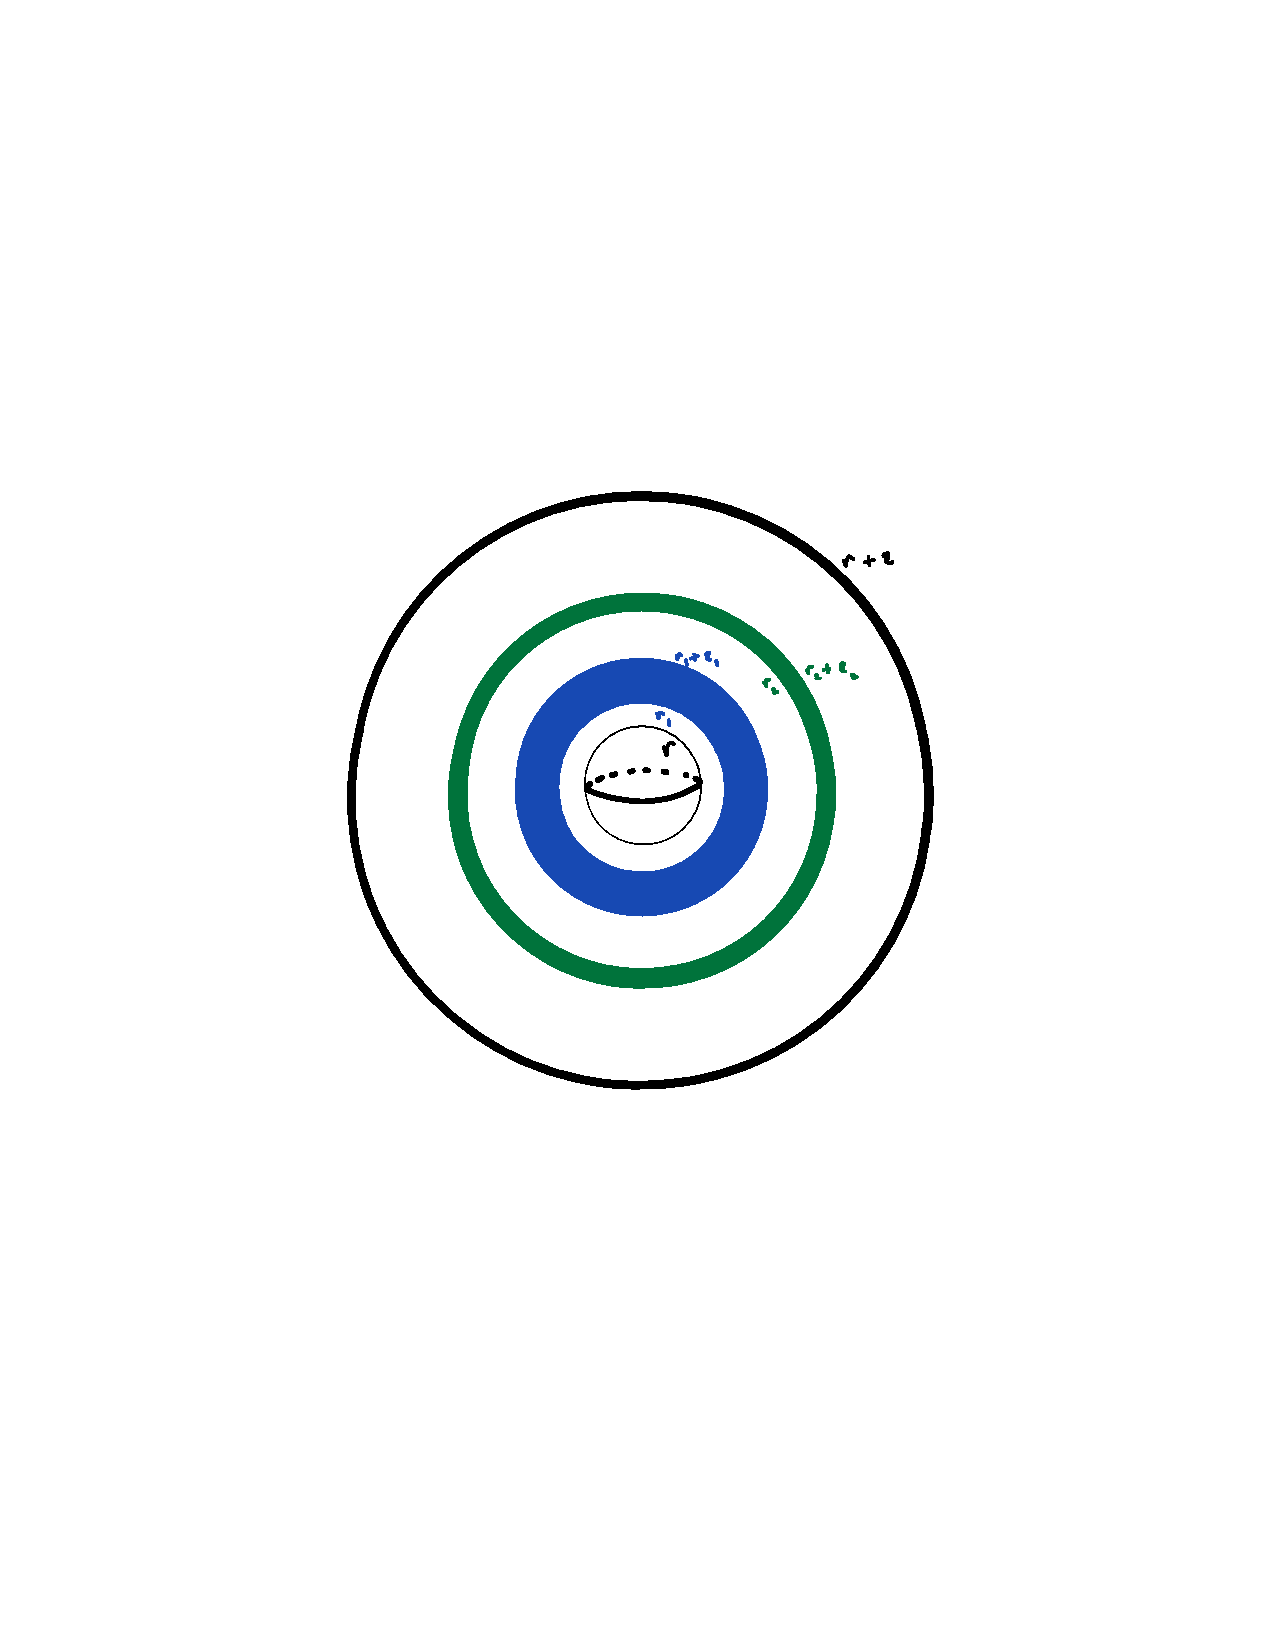
\includepdf[pages=-,pagecommand={},width=\textwidth]{nesting.pdf}
%\end{figure}


\begin{figure}[h]
   \centering
   \begin{tabular}{@{}c@{\hspace{.5cm}}c@{}}
       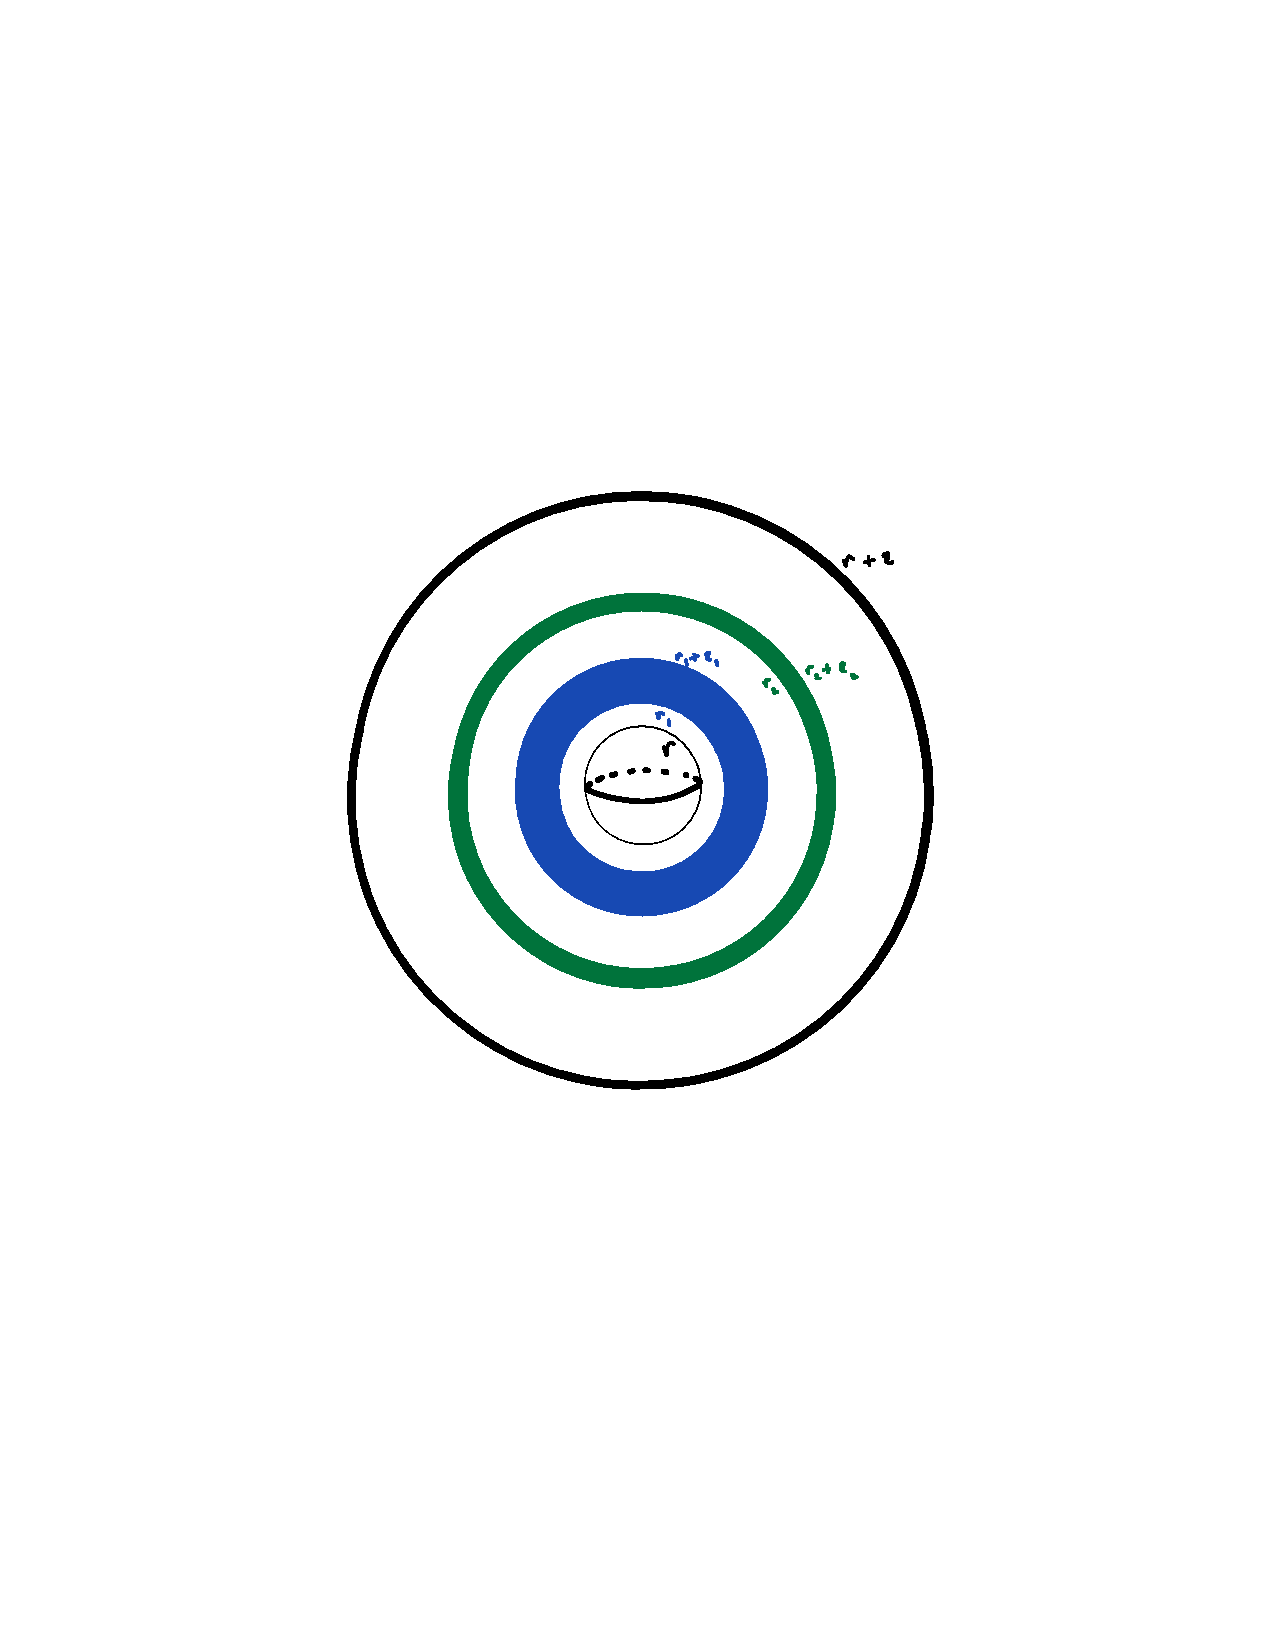
\includegraphics[page=1,width=.45\textwidth]{nesting.pdf} & 
   \end{tabular}
 \caption{Nesting spherical shells. The blue and green shaded regions represent the spherical shells $N_{r_1,\epsilon_1}$ and $N_{r_2,\epsilon_2}$, respectively. The black spheres denote the inner and outer boundaries of the closure of the neighborhood $N_{r,\epsilon}$.}
 \label{fig:nesting}
\end{figure}

The factorization structure map for this embedding of disjoint open sets is of the form 
\be\label{fact product 2}
\Obs^{\q}_{V}(N_{r_1, \epsilon_1}) \tensor \Obs^{\q}_{V}(N_{r_2, \epsilon_2}) \to \Obs^{\q}_{V}(N_{r,\epsilon}) .
\ee
%We will see that the specific choices of $r, r_i$ and $\epsilon, \epsilon_i$ are not important.

\begin{lem} \label{lem sphere alg} The factorization structure map in (\ref{fact product 2}) restricts to the subspace of sphere observables. 
That is, there is a commutative diagram
\ben
\xymatrix{
\Obs^{\q}_{V}(N_{r_1, \epsilon_1}) \tensor \Obs^{\q}_{V}(N_{r_2, \epsilon_2}) \ar[r] & \Obs^{\q}_{V} \\
\sA_V \tensor \sA_V \ar[u] \ar[r]^-{\mu_2} & \sA_V \ar[u]
}
\een
where the top line is the map in (\ref{fact product 2}). 
The same holds for an arbitrary number of nested neighborhoods of the form $N_{r,\epsilon}$. 
That is, for any $k \geq 0$ the factorization product restricts to a linear map 
\ben
\mu_k : \sA_V^{\tensor k} \to \sA_V .
\een
\end{lem}

Each of the neighborhoods $N_{r,\epsilon}$ are contained in the open submanifold $\CC^{d} \setminus \{0\}$.
Note that there is a homeomorphism $\CC^{d} \setminus \{0\} \cong S^{2d-1} \times \RR_{>0}$.
Further, we have the radial projection map
\ben
\pi : \CC^{d} \setminus \{0\} = S^{2d-1} \times \RR_{>0} \to \RR_{>0} 
\een
that sends $z = (z_1,\ldots,z_d) \mapsto |z| = \sqrt{|z_1|^2+\cdots+|z_d|^2}$. 

A fundamental feature of factorization algebras is that they push forward along smooth maps. 
We can thus push forward the factorization algebra $\Obs^\q_V$ on $\CC^{d}\setminus \{0\}$ along $\pi$ to obtain a factorization algebra on $\RR_{>0}$. 
To an open interval of the form $(r-\epsilon, r+\epsilon)\subset \RR_{>0}$ the factorization algebra assigns precisely the observables supported on $N_{r,\epsilon}$. 

Lemma \ref{lem sphere alg} implies that there is a factorization algebra $\sF_{\sA_V}$ associated to $\sA_V$ and that the inclusion $\sA_V \hookrightarrow \Obs^\q(N_{r,\epsilon})$ induces a map of factorization algebras on $\RR_{>0}$:
\ben
\sF_{\sA_V} \to \pi_*(\Obs^\q_V) 
\een
The factorization algebra $\sF_{\sA_V}$ assigns to every interval the dg vector space $\sA_V$. 
In particular $\sF_{\sA_V}$ is locally constant, and hence determines the structure of an $A_\infty$ algebra on $\sA_V$. 
We would now like to identify this algebra structure. 

We will proceed in two ways. 
First, we will use the Moyal formula together with the explicit form of the propagator from Section \ref{sec: remind prop} to deduce the operator product expansion between cohomology classes of operators corresponding to $\sA_V$. 
This will tell us what the algebra structure is on the cohomology $H^*(\sA_V)$. 
Second, we will use the smoothed description of the observables as a factorization enveloping algebra to nail down the precise algebra structure at the cochain level. 

Note that we can view $\sA_V$ as the symmetric algebra on the following cochain complex
\ben
A_d \tensor (V^*[d-1] \tensor V) \oplus \CC \cdot \hbar .
\een
This complex has the structure of a dg Lie algebra, with bracket given by
\be\label{HV bracket}
[\alpha \tensor v^*, \alpha \tensor v] = \hbar \<v^*, v\> \oint_{S^{2d-1}} \alpha \wedge \alpha'  \d^d z .
\ee
All other brackets are determined by graded anti-symmetry and declaring the parameter $\hbar$ is central.
Denote this dg Lie algebra by $\sH_V$. 

Our main result is that the dg algebra structure on $\sA_V$ endowed by the factorization product is equivalent to the universal enveloping algebra $U(\sH_V)$ of the dg Lie algebra $\sH_V$.

\begin{rmk}
If $(\fg, \d, [-,-])$ is a dg Lie algebra its universal enveloping algebra is defined explicitly by 
\ben
U(\fg) = {\rm Tens}(\fg) / (x \tensor y - (-1)^{|x||y|} y \tensor x - [x,y]) .
\een
It is immediate to check that the differential $\d$ descends to one on $U(\fg)$, giving $U(\fg)$ the structure of an associative dg algebra.
\end{rmk}

\subsubsection{Using the Moyal formula}

As eluded to before, we now identify the algebra structure on the cohomology of $\sA_V$
induced by the map of factorization algebras $\sF_{\sA_V} \to \pi_*(\Obs_V^\q)$, where $\sF_{\sA_V}$ is the locally constant factorization algebra that assigns the cochain complex $\sA_V$ to every interval.

Let $\ul{U(\sH_V)}$ be the locally constant factorization algebra on $\RR_{>0}$ based on the associative algebra $U(\sH_V)$. 
We will write down an explicit isomorphism of locally constant factorization algebras
\ben
\Phi : \ul{U(H^*\sH_V)} \to H^*\sF_{\sA_V},
\een
implying the result. 

By Poincar\'{e}-Birkoff-Witt, the dg vector spaces $U(\sH_V)$ and $\sA_V$ are isomorphic. 
Therefore, if $I \subset \RR_{>0}$ is an interval, we define $\Phi(I)$ to be the identity map. 
Thus, it suffices to show that the associative algebra structure on the spherical observables agrees with that of $U(\sH_V)$ in cohomology.

%We also need to take into account a higher operation. 

%If $I_1,I_2$ are two intervals, consider their disjoint union $I_1 \sqcup I_2 \subset \RR_{>0}$. 
%We define
%\ben
%\Phi(I_1 \sqcup I_2) : U(\sH_V) \tensor U({\sH_V}) \to \sF_{\sA_V} (I_1 \sqcup I_2) 
%\een

We turn to an explicit calculation of factorization product for observables in $\pi_*(\Obs_V^\q)$.
If $\sO, \sO' \in U(\sH_V)$ then we can compute the commutator $[\sO,\sO']$ in the factorization algebra as follows.
For $i = 1,2,3$ let $\epsilon_i, r_i > 0$ be such that 
\ben
\epsilon \leq \epsilon_1 < r_1 \leq \epsilon_2 < r_2 \leq \epsilon_3 < r_3 \leq r
\een 
and consider the configurations
\ben
i_{12} : N_{r_1, \epsilon_1} \sqcup N_{r_2, \epsilon_2} \hookrightarrow N_{r, \epsilon}
\een
and
\ben
i_{23} :  N_{r_2, \epsilon_2} \sqcup N_{r_3, \epsilon_3} \hookrightarrow N_{r, \epsilon}
\een
in $\CC^\d \setminus \{0\}$. 
If $I_i = (r_i - \epsilon_i, r_i + \epsilon$ and $I = (r- \epsilon, r+\epsilon)$, these correspond to the configurations $i_{12} : I_1 \sqcup I_2 \hookrightarrow I$ and $i_{23} : I_2 \sqcup I_3 \hookrightarrow I$ in $\RR_{>0}$, respectively. 
The induced factorization structure maps are
\be\label{starprods}
\begin{array}{ccc}
\star_{12} & : & \Obs_V^\q(N_{r_1, \epsilon_1}) \tensor \Obs_V^\q( N_{r_2, \epsilon_2}) \to \Obs_V^\q(N_{r, \epsilon}) \\
\star_{23} & : & \Obs_V^\q(N_{r_2, \epsilon_2}) \tensor \Obs_V^\q( N_{r_3, \epsilon_3}) \to \Obs_V^\q(N_{r, \epsilon}) .
\end{array}
\ee
The commutator $[\sO, \sO']$ is computed via the formula
\be\label{commutator}
\sO \star_{12} \sO' - \sO' \star_{23} \sO .
\ee
In the notation $\sO \star_{12} \sO'$ we view $\sO$ as having support in $N_{r_1,\epsilon_1}$ and $\sO'$ as having support in $N_{r_2,\epsilon_2}$.

We compute this commutator at the level of cohomology.
The cohomology of $A_d$ is concentrated in degrees $0$ and $d-1$. 
Explicitly, one can represent the zeroeth cohomology as
\ben
H^0(A_d) = \CC[z_1,\ldots,z_d] .
\een
Now, let $\omega_{BM}(z,\zbar)$ be the Bochner-Martinelli kernel of type $(0,d-1)$ from above. 
We can express the $(d-1)$st cohomology of $A_d$ as
\ben
H^{d-1}(A_d) = \CC[\partial_{z_1}, \cdots, \partial_{z_d}] \cdot \omega_{BM} 
\een 
That is, every element of $H^{d-1}(A_d)$ can be written as a holomorphic polynomial differential operator acting on $\omega_{BM}$. 
Further, it is convenient to make the $U(d)$-equivariant identification 
\be\label{U(d) identification}
 \CC[\partial_{z_1}, \cdots, \partial_{z_d}] \omega_{BM} \cong z_1^{-1} \cdots z_d^{-1} \CC[z_1^{-1}, \ldots, z_d^{-1}],
 \ee
which makes sense since $\omega_{BM}$ has $T^d \subset U(d)$-weight $(-1,\ldots,-1)$. 

Recall that $\sH_V = A_d \tensor (V^*[d-1] \oplus V)$.
It follows from above that the cohomology of $\sH_V$ is concentrated in degrees $-(d-1), 0, d-1$. 
The non-trivial Lie algebra structure on $\sH_V$ comes from the ordinary symplectic pairing on this space, as we've already discussed. 

Suppose $v,v^*$ are in $V,V^*$, respectively and $\alpha,\alpha' \in A_d$.
The corresponding classical observables $\cO_{\gamma,\alpha}(0;v^*)$ and $\cO_{\beta, z_1^{-1}\cdots z_d^{-1} \alpha'}(0;v)$ have cohomological degrees
\begin{align*}
{\rm deg}\left(\cO_{\gamma,\alpha}(0;v^*)\right) = |\alpha| - d + 1 \\
{\rm deg}\left(\cO_{\beta, z_1^{-1}\cdots z_d^{-1} \alpha'}(0;v)\right) = |\alpha'|,
\end{align*}
where $|\alpha|$ denotes the differential form degree.
In cohomology the only nontrivial form degrees of $\alpha,\alpha'$ that survive are $0,d-1$. 
Suppose that $|\alpha| = 0$.
Then, the only way we could obtain a nontrivial commutator between the operators above is if $|\alpha'| = d-1$. 

We will compute the factorization product in (\ref{commutator}) using our explicit formula for the propagator of the $\beta\gamma$ system computed in Lemma \ref{lem: bm}.
We diverge a moment to recall how this construction works.
The main idea is that the propagator allows us to promote a classical observable to a quantum observable.
Recall, the full propagator is an element
\ben 
P (z,w) = \lim_{L\to \infty} \lim_{\epsilon \to 0} P_{\epsilon < L}(z,w) \in \Bar{\sE}_V(\CC^d) \Hat{\tensor} \Bar{\sE}_V(\CC^d)
\een
where the $\Bar{\sE}_V(\CC^d)$ denotes the space of distributional sections on $\CC^d$.
Explicitly, we showed that 
\ben
P(z,w) = C_d \;\omega_{BM}(z,w) 
\een
where $\omega_{BM}(z,w)$ is the Bochner-Martinelli kernel.

Contraction with $P$ determines a degree zero, order two differential operator
\ben
\partial_{P} : \Obs^{\cl}_V (U) \to \Obs^{\cl}_{V}(U)
\een
for any open set $U \subset \CC^d$. 
Recall that the classical observables on $U$ are simply given by a symmetric algebra on the continuous dual of $\sE_V(U)$. 
Since $\Bar{\sE}^\vee = \sE_c^!$, we can view the propagator as an symmetric smooth linear map
\ben
P^\vee : \sE_{V,c}^!(\CC^d) \Hat{\tensor} \sE_{V,c}^!(\CC^d) \to \CC .
\een
The contraction operator $\partial_P$ is determined by declaring it vanishes on $\Sym^{\leq 1}$, and on $\Sym^2$ is given by the linear map $P^\vee$. 

To compute the factorization product we use the isomorphism
\ben
\begin{array}{cccc}
W_0^\infty : & \Obs^{\cl}_V(U) [\hbar]  & \to & \Obs^\q_V(U) \\
& \cO & \mapsto & e^{\hbar \partial_P} \cO 
\end{array}
\een
that makes sense for any open set $U$.
This is an isomorphism of cochain complexes, with inverse given by $(W_0^\infty)^{-1} = e^{-\hbar \partial_P}$. 
It determines the following formula for the factorization product. 
If $\cO,\cO'$ are observables supported on disjoint opens $U,U'$, and that $W$ is and open set containing $U,U'$, then the factorization structure map is given by
\ben
\cO \star \cO' = e^{-\hbar \partial_P} \left(\left(e^{\hbar \partial_P}\cO\right) \cdot \left(e^{\hbar \partial_P} \cO'\right)\right) \in \Obs^\q_V (W) .
\een 
Here, the $\cdot$ refers to the symmetric product on classical observables.
For a more in depth discussion of this Moyal type formula for factorization algebras see Section 4.3.2 of \cite{CG2}.
For another account, which makes a connection to the usual Moyal formula from deformation quantization see Section 3.5 of \cite{GLL}.
The calculation of the factorization product relies on the higher dimensional residue formula involving the Bochner-Martinelli form. 
If $f$ is any any function in $C^\infty(U)$, where $U$ is a domain in $\CC^d$, then the residue formula states that for any $z \in D$ 
\ben
f(z,\zbar) = \int_{w \in \partial U} \d^d w \; f(w) \; \omega_{BM}(z,w) - \int_{w \in D} \d^d w \; (\dbar f)(w) \wedge \omega_{BM}(z,w) .
\een 
In particular, if $f(z,\zbar)$ is holomorphic the second term drops out and we get the familiar expression for the higher dimensional residue.

We can now perform the main calculation. 
Recall, we have fixed observables $\cO_{\gamma, \alpha}(0;v^*)$ and $\cO_{\beta, z_1^{-1}\cdots z_d^{-1} \alpha'} (0;v)$.
In the notation of Equation (\ref{starprods}), we have
\bestar
\cO_{\gamma, \alpha}(0;v^*) \star_{12} \cO_{\beta, z_1^{-1}\cdots z_d^{-1} \alpha'} (0;v) & = &  \cO_{\gamma, \alpha}(0;v^*) \cdot \cO_{\beta, z_1^{-1}\cdots z_d^{-1} \alpha'} (0;v) \\ & & + \hbar \<v, v^*\>\oint_{|z^1| = r_1} \oint_{|z^2| = r_2} \alpha(z^1) \d^d z^1 \alpha'(z^2) P(z^1,z^2) \\ & = & \cO_{\gamma, \alpha}(0;v^*) \cdot \cO_{\beta, z_1^{-1}\cdots z_d^{-1} \alpha'} (0;v) \\ & & + \hbar \<v, v^*\> \oint_{|z^1| = r_1} \oint_{|z^2| = r_2}  \alpha(z^1) \alpha'(z^2) \d^d z^1 \omega_{BM}(z^1,z^2) \\ & = & \cO_{\gamma, \alpha}(0;v^*) \cdot \cO_{\beta, z_1^{-1}\cdots z_d^{-1} \alpha'} (0;v)  +  \hbar \<v, v^*\> \oint_{|z| = r_1} \alpha(z) \alpha'(z) \d^d z \\ & & +  \hbar \<v, v^*\> \oint_{|z^1| = r_1} \int_{z^2 \in D(0, r_2)} \; \alpha(z^1) (\dbar \alpha')(z^2) \omega_{BM}(z^1,z^2) . 
\eestar 
In the first line we have used the Moyal formula.
In the second line we have used the explicit form of the propagator. 
In the third line we have used the higher residue formula. 
Finally, since we are only interested in the cohomology class of the product, we can assume that $\alpha,\alpha'$ are both holomorphic. 
In particular, the third term in the last line vanishes. 
The calculation for the $\star_{23}$ product is similar. 
We conclude that in cohomology the commutator between the quantum observables $\cO_{\gamma, \alpha}(0;v^*)$ and $\cO_{\beta, z_1^{-1}\cdots z_d^{-1} \alpha'} (0;v)$ is precisely
\ben
\hbar \<v, v^*\> \oint_{|z| = r_1} \alpha(z) \alpha'(z) \d^d z .
\een
This agrees with the commutator $(\ref{HV bracket})$ in $\sH_V$. 
The extension to commutators between non-linear observables is completely analogous. 
Thus, we conclude that as associative graded algebras one as 
\ben
U(H^* \sH_V) \cong H^* \sA_V .
\een

\subsubsection{Using smoothed observables}

We now provide a refined description of the algebra of sphere operators, yet this approach may seem more indirect. 
It relies on interpreting the observables of the $\beta\gamma$ system as the {\em factorization envelope} of a certain sheaf of Lie algebras.

The linear smoothed observables, equipped with the linearized BRST differential, on any $U \subset \CC^d$ form the subcomplex 
\ben
\Omega^{d,*}_c(U) \tensor V^*[d] \oplus \Omega_c^{0,*} (U) \tensor V [1] \subset \Obs^{\cl}_V(U) .
\een
Using the $P_0$ bracket restricted to the linear observables, we can form the central extension of dg Lie algebras
\ben
0 \to \CC [-1] \cdot \hbar \to \sH'_V(U) \to \Omega^{d,*}_c(U) \tensor V^*[d] \oplus \Omega^{0,*} (U) \to 0 .
\een
This is similar to the construction of the ordinary Heisenberg algebra (such as $\sH_V$ above).
For classical linear observables the Lie bracket is defined by $[\cO, \cO'] = \hbar \{\cO, \cO'\}$, where $\{-,-\}$ is the $P_0$ bracket. 
Since the $P_0$ bracket is degree $+1$ to make this a dg Lie algebra we must put $\hbar$ in degree $+1$ as well.
Note that this construction works well as we vary the open set $U$. 
Namely, $U \mapsto \sH'_V(U)$ is a cosheaf of Lie algebras on $\CC^d$. 
An elementary observation identifies the smoothed quantum observables with the factorization enveloping algebra of $\Tilde{\sH}_V$:
\ben
\Obs^{\q}_{V} \cong \UU(\sH'_V) .
\een
Indeed, the right hand side assigns to each open $U$ the cochain complex $\clieu_*(\Tilde{\sH}_V(U)) = \left(\Sym(\sH_V'(U)), \dbar + \d_{CE}\right)$. 
One checks directly that $\d_{CE}$ is precisely the BV Laplacian $\hbar \Delta$. 

%We now introduce the following algebra, which is a deformation of the associative dg algebra $U(\sH_V)$ from the previous section.
%Let $\Tilde{\sH}_V$ denote the following extension of dg Lie algebras
%\ben
%0 \to \CC \cdot \hbar \to \Tilde{\sH}_V \to A_d \tensor (V^*[d-1] \tensor V) \to 0
%\een
%determined by the $2$-cocycle
%\ben
%(\alpha \tensor v^* , \alpha' \tensor v) \mapsto \hbar \<v,v^*\> \oint_{S^{2d-1}} \alpha \alpha' \d^d z + \hbar \<v, v^*\> \oint_{z \in S^{2d-1}} \alpha(z) \d^d z \int_{w \in D} \dbar \alpha' (w) \omega_{BM}(z,w)  + (\alpha \leftrightarrow \alpha') .
%\een 
%%To check that this is a cocycle, note that by the residue formula one has 
%%\ben
%%\oint_{z \in S^{2d-1}} \dbar \alpha(z) \d^d z \int_{w \in D} \dbar \alpha'(w) \omega_{BM}(z,w) = ...
%%\een
%The first term above defined the bracket for $\sH_V$, so we are deforming the bracket by the second term. 
%\brian{call $\Tilde{\sA}_V$ the algebra with commutator that includes the error term in the residue}.

%\ben
%\xymatrix{
%\Obs^{\q, sm}(N_{r,\epsilon}) \ar@{^{(}->}[r] & \Obs^\q_V(N_{r,\epsilon}) \\
%\sA_V \ar@{.>}[u] \ar[ur]_-{i_{S^{2d-1}}} .
%}
%\een

\begin{prop}
There is a locally constant factorization algebra $\sF_V$ on $\RR_{>0}$ with the following properties:
\begin{enumerate}
\item $\sF_V$ admits a map of factorization algebras
\ben
\sF_V \to \rho_* (\Obs^\q_V)
\een
that is dense at the level of cohomology.
\item As a locally constant one-dimensional factorization algebra $\sF_V$ is equivalent to the dg algebra $U(\sH_V)$. 
\end{enumerate}
\end{prop}

\begin{proof}
We will write down the factorization algebra $\sF_V$ and then prove the above two properties we claim it satisfies. 
Consider the local Lie algebra on $\RR_{>0}$ whose compactly supported sections are $\Omega^*_{\RR_{>0},c} \tensor \sH_V$.
The Lie bracket is encoded by the Lie bracket on $\sH_V$ combined with the wedge product of forms on $\RR_{>0}$. 
Now, we define $\sF_V$ as the factorization envelope of this local Lie algebra 
\ben
\sF_V = \UU\left(\Omega^*_{\RR_{>0},c} \tensor \sH_V\right) .
\een
By construction, $\sF_V$ is locally constant and equivalent, as an associative dg algebra, to $U(\sH_V)$. 
Thus, we must only show part (1). 

We have just expressed $\Obs_V^\q$ as a factorization enveloping algebra as well.
Since the pushforward commutes with the functor $\UU(-)$, to construct the map in (1) it suffices to provide a map of factorization Lie algebras
\ben
\Phi : \Omega^*_{\RR_{>0},c} \tensor \sH_V \to \rho_* \sH_V' .
\een
Recall that as a vector space $\Tilde{\sH}_V = A_d \tensor (V^*[d-1] \oplus V)$.
Let $I \subset \RR_{>0}$ be an open subset, we will describe the map $\Phi(I)$.
There is the natural map $\rho^* : \Omega^*_c(I) \to \Omega^*_c(\rho^{-1}(I))$ given by the pull back of differential forms. 
We can post compose this with the natural projection ${\rm pr}_{\Omega^{0,*}} : \Omega^*_c \to \Omega^{0,*}_c$ to obtain a map of commutative algebras ${\rm pr}_{\Omega^{0,*}} \circ \rho^* : \Omega^*_c(I) \to \Omega^{0,*}_c(\rho^{-1}(I))$. 
The map $j$ from Proposition \ref{prop: Ad} determines a map of dg commutative algebras $j : A_d \to \Omega^{0,*}(\rho^{-1}(I))$. 
Thus, we obtain a map
\ben
\begin{array}{cccc}
\Phi(I) = ({\rm pr}_{\Omega^{0,*}} \circ \rho^*) \tensor j \tensor {\rm id}_V : & \Omega^*_c(I) \tensor A_d \tensor V & \to & \Omega^{0,*}_c\left((\rho^{-1}(I)\right) \tensor V \\
& \varphi \tensor a \tensor v & \mapsto & \left(\left(({\rm pr}_{\Omega^{0,*}} \circ \rho^*) \varphi\right) \wedge j(a) \right) \tensor v
\end{array}
\een
Note that since the map $j$ is a dense map in cohomology so is $\Phi(I)$ for each $I \subset \RR_{>0}$.
The map on the $A_d \tensor V^*[d-1]$ component of $\sH_V$ is defined similarly.
Moreover, on the central factor $\hbar \Omega^*_c(I) \subset \Omega^*_{\RR_{>0},c} \tensor \sH_V$ we define
\ben
\Phi(I) (\hbar \varphi) = \hbar \int_I \varphi .
\een

To show that this is a map of cosheaves of dg Lie algebras we must show that the differentials and brackets are compatible.
The differential on $\sH_V$ is $\d_{dR, \RR} + \dbar$ where $\dbar$ is the differential on $A_d$. 
Let $\varphi \tensor a \tensor v^*$ be an element in $\Omega^*(I) \tensor A_d \tensor V^*[d-1]$. 
The differential applied to this element is
\ben
\frac{\partial \varphi}{\partial r} \d r \tensor a \tensor v^* + \varphi \tensor \dbar a \tensor v^* .
\een
Under $\Phi(I)$ this element gets mapped to
\ben
\sum_i \frac{\partial \varphi}{\partial r} \frac{z_i}{2r} \d \zbar_i \wedge a(z,\zbar) \tensor v^* + \varphi (r) \wedge \dbar a (z,\zbar) \tensor v^* .
\een
To see that the differentials are compatible, we note that when acting on functions $\varphi(r)$ that only depend on the radius, one has $\frac{\partial \varphi}{\partial \zbar_i} = \frac{z_i}{2r} \frac{\partial \varphi}{\partial r}$. 
The fact that the differentials are compatible follows immediately. 

Now, suppose $\varphi \tensor a \tensor v^* \in \Omega^*_c(I) \tensor A_d \tensor V^*[d-1]$ and $\psi \tensor b \tensor v \in \Omega^*_c(I) \tensor A_d \tensor V$.
The Lie bracket in $\sH_V$ of these elements is
\be\label{bracket1}
[\varphi \tensor a \tensor v^*, \psi \tensor b \tensor v]_{\sH_V} = \hbar \<v,v^*\> \int_I \varphi \psi \oint a b \d^d z .
\ee
Now, using the definition of the $(-1)$-shifted symplectic structure defining the free $\beta\gamma$ system, we have
\begin{align*}
[\Phi(I)(\varphi \tensor a \tensor v^*), \Phi(I)(\psi \tensor b \tensor v)]_{\sH_V'} & = \hbar \<v,v^*\> \int_{\rho^{-1}(I)} \phi(r) a(z,\zbar) \psi(r) b(z,\zbar)\d^d z \\  & = \hbar \<v,v^*\> \int_{r \in I} \phi(r) \psi(r) \oint_{S^{2d-1}_r} a(z,\zbar) b(z,\zbar) \d^d z . 
\end{align*}
This is precisely the image of the right hand side of (\ref{bracket1}) under $\Phi(I)$. 
Thus, $\Phi$ determines a map of cosheaves of Lie algebras.
By functoriality of the enveloping factorization algebra together with compatibility under pushforward $\UU(\rho_* \sF) \cong \rho_* \UU(\sF)$, we obtain a map of factorization algebras
\ben
\Phi : \sF_V = \UU\left( \Omega^*_{\RR_{>0},c} \tensor \sH_V \right) \to \rho_* \UU (\sH_V') = \rho_* \Obs^\q_V .
\een
That this map is dense in cohomology follows from Proposition \ref{prop: Ad} in the Appendix \ref{chap: appendix}.
\end{proof}


%\begin{rmk}
%At the level of cohomology $H^*(\Tilde{\sA}_V) \cong H^*(\sA_V)$ as graded algebras....\brian{comment}
%\end{rmk}



\subsection{The disk as a module}\label{sec: disk module}
In the beginning of this section we extracted a subspace of the cohomology of the observables on the $d$-dimensional disk 
\ben
\sV_V \subset \Obs^{\q}_{V} (D(0,r))
\een
by looking at the $U(d)$ weight spaces. 
We have also seen how the factorization product endows a subspace of the observables supported on neighborhoods of spheres $S^{2d-1} \subset N_{\epsilon, r}$
\ben
\sA_V \subset \Obs^\q_V (N_{\epsilon,r})
\een
with the structure of a associative dg algebra.
In this section we study a different part of the factorization algebra structure that equips $\sV_V$ with the structure of a module over $\sA_V$. 
Moreover, we will identify this module structure in a way that is reminiscent of the state space of a vertex algebra in the world of CFT.

First, we describe the factorization structure map for a very simple configuration of open sets. 
Suppose $R > r + \epsilon$ and consider the inclusion 
\be\label{NtoD}
N_{r,\epsilon} \hookrightarrow D(0, R) .
\ee
This configuration induces the following diagram
\be\label{composition1}
\begin{tikzcd}
\sA_V \arrow[d, hook] \arrow[r, dashed] & \sV_V \arrow[d, hook] \arrow[r,"H^*(-)"] & H^*(\sV_V) \arrow[d, hook] \\
\Obs^\q_V(N_{r,\epsilon}) \arrow[r,"\mu"] & \Obs^\q_V(D(0,R)) \arrow[r,"H^*(-)"] & H^*\left(\Obs^\q_V(D(0,R))\right).
\end{tikzcd}
\ee
The bottom arrow is the factorization structure map from (\ref{NtoD}) followed by the projection $H^*(-)$ onto cohomology.
Note that projection is well-defined since the cohomology is concentrated in the top degree. 
The vertical arrows are all the inclusions of the $U(d)$-eigenspaces where we recall that the state space $\sV_V$ embeds inside the cohomology of the observables on a disk.
We will see in the next lemma that the map $\mu$ factors through $\sV_V$, hence producing the dashed arrow $\sA_V \to \sV_V$.

To state the lemma, recall the presentation for the cohomology of the commutative dg algebra $A_d$ in terms of the Bochner-Martinelli kernel.
Following Remark \ref{rmk: Ad}, we use the $U(d)$-equivariant presentation
\ben
H^{d-1}(A_d) = \CC\left[\frac{\partial}{\partial z_1}, \ldots, \frac{\partial}{\partial z_d}\right] \omega^{alg}_{BM} ,
\een
where, on the right hand side we take the cohomology class.
This says that every cohomology class may be represented by some constant coefficient holomorphic differential operator applied to $\omega^{BM}$.
%In the \v{C}ech notation, we express the cohomology $H^{d-1} (A_d) = z_1^{-1} \cdots z_d^{-1} \CC[z_1^{-1}, \ldots,z_d^{-1}]$. 
%There is a $U(d)$-equivariant relationship between these two descriptions which sends $\omega^{BM} \leftrightarrow z_1^{-1} \cdots z_d^{-1}$. 

\begin{lem}\label{lem: N to D}
There exists a lift of $\mu$ making the diagram (\ref{composition1}) commutative.
In particular there exists a map $\pi_- : \sA_V \to H^*\sV_V$ compatible with the factorization structure maps. 
This is a map of symmetric algebras, further on linear elements $a \tensor v^*, b \tensor v \in A_d \tensor (V^*[d-1] \oplus V) \subset \sA_V$ the map is
\ben
\pi_-(a \tensor v^*) = 
\begin{cases}
    \cO_{\gamma, -\vec{n}}(0;v^*) ,& \text{if } |a| = d-1 \\
    0,              & \text{otherwise} .
\end{cases}
\een
and
\ben
\pi_-(b \tensor v) = 
\begin{cases}
    \cO_{\beta, -\vec{m}}(0;v) ,& \text{if } |b| = d-1 \\
    0,              & \text{otherwise} .
\end{cases}
\een
Where, $a = (\frac{\partial}{\partial z})^{\vec{n}} \omega^{BM} \in A^{d-1}_d$ and $b = (\frac{\partial}{\partial z})^{\vec{m}} \omega^{BM} \in A^{d-1}_d$.
\end{lem}

The notation $\pi_-$ will become apparent momentarily.

\begin{proof}
For degree reasons it is automatic that in the composition in (\ref{composition1}) is only nonzero on $a\tensor v^*, b \tensor v \in A_d\tensor (V^*[d-1] \oplus V)$ if $|a|=|b|=d-1$. 
Since $\omega^{BM}$ is $U(d)$ invariant, it is clear that the element $a = \partial^{\vec n} \omega^{BM}$ it lives in the weight $-\vec{n}$ subspace and defines the observable 
\ben
\gamma \tensor v \mapsto \<v,v^*\> \oint_{S^{2d-1}} \gamma(z,\zbar) (\frac{\partial}{\partial z})^{\vec{n}} \omega^{BM} \d^d z .
\een
Since we are only interested in the cohomology class, we can assume that $\gamma$ is holomorphic.
In this case, the residue formula implies that this is precisely the observable $\cO_{\gamma 
; -\vec{n}} (0 ; v^*)$. 
The argument for $b \tensor v$ is similar.
\end{proof}

We consider the configuration of open sets of a small $d$-disk enclosed by a neighborhood $N_{\epsilon, r}$. 
Concretely, suppose $r_1 < r_2 -\epsilon < r_2 + \epsilon < R$ and consider the inclusion of opens
\be\label{open module}
D(0,r_1) \sqcup N_{\epsilon, r_2} \hookrightarrow D(0,R). 
\ee
Consider the following diagram
%\ben
%\xymatrix{
%\Obs^\q_V (D(0,r_1)) \tensor \Obs^\q_V(N_{\epsilon,r_2}) \ar[r]^-%{\mu} & \Obs^\q_V(D(0,R)) \ar[d]^-{H^*(-)} \\
%\Obs^\q_V(D) \tensor \sA_V \ar[u] \ar[r]^-{\mu|_{\sA_V}} & H^*(\Obs^\q_V(D(0,R))) \\
%\sV_V \tensor \sA_V \ar[u] \ar@{.>}[r] & \sV_V \ar[u] .
%}
%\een

\ben
\xymatrix{
\Obs^\q_V (D(0,r_1)) \tensor \Obs^\q_V(N_{\epsilon,r_2}) \ar[r]^-{\mu} & \Obs^\q_V(D(0,R)) \\
\Obs^\q_V(D) \tensor \sA_V \ar[u] & \\
\sV_V \tensor \sA_V \ar[u] \ar@{.>}[r] & \sV_V \ar[uu] .
}
\een

The top horizontal line $\mu$ is the factorization structure map coming from the configuration in (\ref{open module}).

%The map $H^*(-)$ is simply the quotient map onto the cohomology.

%The map $\mu|_{\sA_V}$ is simply the composition of $\mu$ with this quotient map onto cohomology.
All of the upward pointing vertical arrows are the inclusions of $\sA_V, \sV_V$ into the sphere and disk observables, respectively. 
We claim that the bottom horizontal arrow exists; that is, the restricted factorization product factors through $\sV$. 
This follows from the fact that the factorization structure map preserves the $U(d)$-eigenspaces.

We have seen that the commutative dg algebra $A_d$ has cohomology concentrated in degrees $0$ and $d-1$.
Since the complex is concentrated in degrees $0,\ldots,d-1$ there exists a quotient map $q : A_d \to H^{d-1}(A_d)$. 
In the remainder of the section we use the notation $A_{d,-} := H^{d-1}(A_d)$.
In addition, let $A_{d,+}$ denote the kernel of this map $A_{d,+} = \ker (q) \subset A_d$. 

Correspondingly, there is an abelian dg Lie subalgebra
\ben
\sH_{V,+} = A_{d,+} \tensor (V^*[d-1] \oplus V) \subset \sA_V 
\een
and a commutative subalgebra $\sA_{V,+} = U(\sH_{V,+}) \subset \sA_V$. 
In fact, this is a maximal commutative subalgebra of $\sA_V$. 
Using $A_{d,-}$ we can similarly define the cochain complex $\sH_{V,-} = A_{d,-} \tensor (V^*[d-1] \oplus V)$. 
As cochain complexes there is a splitting $\sH_V = \sH_{V,+} \oplus \sH_{V,-}$.
Hence, by the PBW theorem there is a splitting $\sA_{V} = \sA_{V,+} \tensor \sA_{V,-}$ as cochain complexes.
The induction of the trivial $\sA_{V,+}$-module $\CC$ to a $\sA_V$-module is given by $\sA_V \tensor_{\sA_{V,+}} \CC$. 
We will refer to this as the {\em vacuum} $\sA_V$-module. 
There is a canonical element $|0\> = 1 \tensor 1 \in \sA_V \tensor_{\sA_{V,+}} \CC$.

\begin{prop}
The factorization product corresponding disks enclosed by the neighborhoods $N_{r,\epsilon}$ endows the state space $\sV_V$ the the structure of a module over the dg algebra $\sA_V$. 
Moreover, as $\sA_V$-modules there is a quasi-isomorphism
\ben
\sV_V \simeq \sA_V \tensor_{\sA_{V,+}} \CC
\een
which sends the unit observable $1 \in \sV_V$ to the vacuum element $|0\>$. 
\end{prop}

\begin{proof}
First, note that there is a map of cochain complexes $\sA_V \to \sV_V$ sending an element of the algebra $a$ to its action on the unit observable $a \cdot 1 \in \sV_V$. 
By the unit axiom for factorization algebras, this maps fits into a commutative diagram
\ben
\begin{tikzcd}
\sA_V \arrow[r] \arrow[d] & \Obs^\q_V(N_{\epsilon,r}) \arrow[d,"\mu"] \\
\sV_V \arrow[r] & \Obs^\q_V(D(0,R)) .
\end{tikzcd}
\een
By Lemma \ref{lem: N to D} we know that if $a \in \sA_{V,+}$ then $a \cdot 1$ is homotopically trivial in $\sV_V$. 
Thus, $\sA_V \to \sV_V$ descends to a map of $\sA_V$-modules $\sA_V \tensor_{\sA_{V,+}} \CC \to \sV_V$.

It remains to see that this is a quasi-isomorphism.
It suffices to show that $H^*(\sA_{V,-}) \cong H^*(\sV_V)$.
The map $\sA_V \to \sV_V$ preserves the filtration by symmetric degree, so it defines a map ${\rm Gr} H^*(\sA_V) \to {\rm Gr} H^*(\sV_V)$.
The cohomology of the state space $\sV_V$ sits inside the cohomology of the disk observables as the $U(d)$-invariants. 
At the level of the associated graded this embedding is
\ben
{\rm Gr} H^*(\sV_V) \subset \Sym\left( \left(\sO^{hol}(D(w,r)\right)^\vee \tensor V^* \oplus \left(\Omega^{d,hol}(D(w,r))\right)^\vee\tensor V[-d+1] \right) [\hbar] .
\een
The right-hand side is the associated graded of the cohomology of the disk observables which we computed in Lemma \ref{lem: disk cohomology}.
Consider the topological vector space $\sO^{hol}(D(w,r))^\vee$. 
Using the holomorphic volume form $\d^d z$ the higher residue pairing defines a map $H^{d-1}(A_d) \to \sO^{hol}(D(w,r))^\vee$ which is an isomorphism after taking $U(d)$-eigenspaces
Similarly, residue pairing defines a map $H^{d-1}(A_d) \to (\Omega^{d,hol}(D(w,r)))^\vee$ which is an isomorphism at the level of $U(d)$-eigenspaces. 
Thus, we can identify the map ${\rm Gr} H^*(\sA_V) \to {\rm Gr} H^*(\sV_V)$ with the map
\ben
\Sym(\d^d z H^*(A_d) \tensor V^*[d-1] \oplus H^*(A_d) \tensor V)[\hbar] \to \Sym(\d^d z H^{d-1}(A_d) \tensor V^* \oplus H^*(A_d)\tensor V [-d+1]) [\hbar] 
\een
induced by the projection $H^*(A_d) \to H^{d-1}(A_d) [-d+1] = \sA_{d,-}$ as desired.
\end{proof}


%Recall that $\sA_V$ is isomoprhic to the enveloping algebra of the Heisenberg dg Lie algebra 
%\ben
%\sH_V = A_d \tensor (V^*[d-1] \tensor V) \oplus \CC \cdot \hbar .
%\een
%Now, the cohomology of the dg Lie subalgebra $\sH_{V,-} \subset \sH_V$ is $H^{d-1}(A_d) 

\begin{rmk}
The subalgebra of sphere operators $\sA_{V,+}$ is the higher dimensional generalization of ``annihilation operators" in the context of CFT. 
Repeated application of these operators kills any vector in $\sV_V$.
Similarly, the quotient $\sA_{V,-}$ is the collection of "creation operators". 
One obtains the entire $\sA_V$-module by applying elements of $\sA_{V,-}$ to the vacuum element $|0\>$. 
\end{rmk}

%\begin{lem} 
%Consider the factorization algebra structure map for the inclusion $N_{r, \epsilon}(w) \hookrightarrow D(w, R)$ where $R > r + \epsilon$:
%\ben
%\mu : \Obs^\q_V(N_{r,\epsilon}(w)) \to \Obs^\q_V(D(w,R)) .
%\een
%Then, in cohomology $H^*(\mu)|_{H^* \sA_V}$ is only nonzero on elements in
%\ben
%\Sym \left(H^{d-1}(A_d) \tensor (V^*[d-1] \oplus V)\right) .
%\een
%On the linear elements inside of this symmetric algebra, the factorization map map satisfies
%\ben
%H^* \mu : \cO_{\gamma , \partial_z^{\vec{n}} \omega_{BM}} \mapsto \cO_{\gamma, -\vec{n}}
%\een
%\end{lem}
%
%\begin{prop}
%The factorization product above gives the cohomology $H^*\sV_V$ the structure of a graded module for the associative graded algebra $H^*\sA_V$.
%Moreover, there is an isomorphism of $H^*\sA_V$ modules
%\ben
%H^*\sV \cong H^*\sA_V \tensor_{\sA_{V,+}} \CC .
%\een 
%\end{prop}
%
%The tensor product $H^*\sA_V \tensor_{\sA_{V,+}} \CC$ is equal to the induction of the trivial module along the subalgebra $\sA_{V,+} \subset H^*\sA_V$. 
%In particular, it implies that as a graded vector space
%\ben
%H^* \sV_V \cong \sA_{V,-} [-d+1],
%\een
%which is immediate from our identification (\ref{U(d) identification})

\subsection{A formula for the character}

In this section we compute the character of the action of $U(d) \times U(1)_f$ on the local observables of the free $\beta\gamma$ system with values in $V$. 
We have already seen that the quantum theory is equivariant for this group, so it makes sense to compute such a character.
By definition, the character is conjugation invariant, so it is completely determined by its value on the subgroup $T^d \times U(1)_f \subset U(d) \times U(1)_f$. 
Choose the following basis for the maximal torus of $U(d)$: 
\ben
T^d = \{{\rm diag}(q_1,\ldots,q_d) \; | \; |q_i| = 1\} \subset U(d).
\een 
We label the generator of $U(1)_f$ by $u$. 
%\brian{something about filtrations. I.e., why does the "formal character" make sense?} 
We view the character as an element in the power series ring $\CC[[q_i^{\pm}, u^{\pm q_f}]]$. 

We will perform the detailed calculation in the case that the complex dimension $d = 2$, with an aim to compare to the formula for the character of the $\cN = 1$ supersymmetric chiral multiplet on $\RR^4$. 
The higher dimensional calculation is similar, and the result is given following the two dimensional calculation.

The local operators of the theory we are those supported on the disk $D^2 \subset \CC^2$. 
Since the theory is translation invariant it suffices to consider a disk centered at the origin $0 \in \CC^2$. 
When $d=2$ we use Lemma \ref{lem: disk cohomology} to read off the cohomology of the disk observables $H^*\Obs^\q_V (D^2)$:
\ben
\Sym\left((\sO^{hol}(D^2) \tensor V)^\vee \right) \tensor \Sym \left( (\Omega^{2,hol}(D^2) \tensor V^*)^\vee [-1] \right) .
\een 

\begin{prop} The $U(2) \times U(1)_f$ character of the local operators of the $\beta\gamma$ system on $\CC^2$ is equal to the elliptic $\Gamma$-function
\ben
\Gamma_{ell}(u ; q_1,q_2) = \prod_{n_1, n_2 \geq 0} \frac{1 - u^{q_f} q_1^{n_1 - 1} q_2^{n_2 - 1}}{1 - u^{-q_f} q_1^{n_1} q_2^{n_2}} \in \CC[[q_1^{\pm},q_2^{\pm}, u^{\pm q_f}]] .
\een
\end{prop}

For an introduction to the elliptic $\Gamma$-function and other related hypergeometric series we refer to the textbook reference \cite{Gasper}. 

\begin{proof}
We recall the basis for a $U(2)$-eigenspaces of the observables on a $2$-disk that we described in Section \ref{sec: disk obs}.
Fix non-negative integers $n_1,n_2 \geq 0$ and elements $v \in V$, $v^* \in V^*$ consider the following linear observables on the $2$-disk:
\ben
\begin{array}{ccclll} 
O_{\gamma} (n_1,n_2 ; v^*) & : & \gamma \tensor w & \in \sO^{hol}(D^2) \tensor V & \mapsto & \ev(v^*, w) \frac{\partial^{n_1}}{\partial z_1^{n_1}} \frac{\partial^{n_2}}{\partial z_2^{n_2}} \gamma (0) \\
O_{\beta} (n_1+1,n_2+1; v) & : & \beta \d z_1 \d z_2 \tensor w^* & \in \Omega^{2,hol} (D^2) \tensor V^* & \mapsto & \ev(w^*, v) \frac{\partial^{n_1}}{\partial z_1^{n_1}} \frac{\partial^{n_2}}{\partial z_2^{n_2}} \beta (0) .
\end{array} 
\een

%Since the field $\gamma \tensor w \in \sO^{hol} \tensor V$ has $U(2)$ weight zero, we see that the \brian{what?}

For fixed $n_1,n_2 \geq 0$, let $V^*_{n_1,n_2}$ denote the linear span of operators $O_{\gamma}(n_1, n_2; v^*)$. 
As a vector space $V_{n_1,n_2}^* \cong V^*$, but we want to remember the weights under $U(2)$. 
Likewise, for $n_1 , n_2 > 0$, let $V_{n_1,n_2} \cong V$ be the linear span of the operators $O_{\beta}(n_1, n_2 ; v)$. 

There is an injective map of graded vector spaces
\ben
\Sym \left( \left(\bigoplus_{n_1,n_2 \geq 0} V_{n_1,n_2}^*\right) \oplus \left(\bigoplus_{n_1,n_2 > 0}  V_{n_1,n_2}[-1] \right)\right)  \to \Sym\left( \left(\sO^{hol}(D^2) \tensor V\right)^\vee \oplus \left( \Omega^{2,hol}(D^2) \tensor V^*\right)^\vee [-1] \right),
\een
where the right-hand side is the cohomology of the observables on $D^2$ and the left-hand side is the cohomology of the state space that we denoted $H^*\sV_V$ in Section \ref{sec: disk obs}. 

Thus, to compute the character of the local operators it suffices to compute it on the vector space
\ben
\Sym \left( \left(\bigoplus_{n_1,n_2 \geq 0} V_{n_1,n_2}^*\right) \oplus \left(\bigoplus_{n_1,n_2 > 0} \oplus V_{n_1,n_2}[-1] \right)\right) \cong \Sym \left(\bigoplus_{n_1,n_2 \geq 0} V_{n_1,n_2}^*\right) \tensor \Wedge \left(\bigoplus_{n_1,n_2 > 0} V_{n_1,n_2} \right) .
\een
We have used the convention that as (ungraded) vector spaces the symmetric algebra of a vector space in odd degree is the exterior algebra. 
For instance, $\Sym(W[-1]) = \Wedge(W)$ as ungraded vector spaces. 
We can further simplify the right-hand side as
\ben
\bigotimes_{n_1, n_2 \geq 0} \left(\Sym(V^*_{n_1,n_2})\right) \bigotimes \bigotimes_{n_1,n_2 > 0} \left(\Wedge (V_{n_1,n_2})\right) .
\een 
The character of the symmetric algebra $\Sym(V^*_{n_1,n_2})$ is equal to $(1-u^{-q_f}q_1^{n_1}q_2^{n_2})^{-1}$ and the character of $\Wedge(V_{n_1,n_2})$ is equal to $(1- u^{q_f} q_1^{n_1}q_2^{n_2})$. 
The formula for character in the statement of the proposition follows from the fact that the character of a tensor product is the product of the characters. 
\end{proof}

Our expression for the character of the local operators of the $\beta\gamma$ system on $\CC^2$ agrees with the partition function of the $\cN = 1$ supersymmetric chiral multiplet on the manifold $S^3 \times S^1$, computed in \cite{Closset1}.
There is the following mathematical explanation for this.
The free $\beta\gamma$ system on $\CC^2$ is equivalent to the holomorphic twist of the free $\cN=1$ chiral multiplet in four dimensions. 
Recall that the data of a twist of a supersymmetric theory, as explained in \cite{CostelloHolomorphic} is that of a supercharge $Q$ that satisfies $Q^2 = 0$. 

\begin{prop}\label{prop: twist}
Consider the $\cN = 1$ chiral multiplet on $\RR^4$.
There is a unique (up to rotation) nontrivial $SU(2)$-invariant supercharge $Q$ satisfying $Q^2 = 0$. 
The twist of the $\cN=1$ chiral multiplet with respect to $Q$ is equivalent to the free $\beta\gamma$ system on $\CC^2$.
If one turns on a $\CC^\times$-invariant superpotential $V$, the twist is equivalent to the holomorphic $\sigma$-model with target the critical locus of $V$.
\end{prop}

We will prove this proposition in a subsequent publication.

\begin{rmk}
One should compare this to the standard situation for two-dimensional supersymmetric $\sigma$-models.
The two-dimensional $\cN = (2,0)$ theory admits a unique nontrivial holomorphic twist which is equivalent to the curved $\beta\gamma$ system on Riemann surfaces. 
There are many verifications of this in the physics literature, see \cite{WittenCDO} for the original discussion. 
For a mathematical proof, see the forthcoming paper with Gwilliam and Szczesny \cite{GSW}.\footnote{In fact, Proposition \ref{prop: twist} implies this.}
It is the $\cN = (2,2)$ $\sigma$-model that admits two further topological twists, these are the $A$ and $B$-models.
\end{rmk}

The supersymmetric partition function of the $\cN=1$ is closed for the supercharge $Q$, thus one expects it to survive under the holomorphic twist.
This is, indeed, exactly what we find.
In \cite{Closset1} Equation 5.58 the partition function for the $\cN=1$ chiral multiplet on $S^3 \times S^1$ is computed, and our answer of the local character of the holomorphic twist is easily seen to agree with theirs. 
We conclude that in this instance that under the holomorphic twist the supersymmetric partition function on $S^3 \times S^1$ was sent to the character of the local observables of the holomorphic theory. 
In future work our goal is to show that this is a general phenomena of superconformal indices.

Without much more difficulty, one can obtain the formula for the character of the holomorphic $\sigma$-model of maps $\CC^d \to V$ for any $d$.

\begin{prop} The $U(d) \times U(1)_f$ character of the local operators of the holomorphic $\sigma$-model of maps $\CC^2 \to V$ is equal to the formal series
\ben
\prod_{n_1,\ldots,n_d \geq 0} \frac{1 - u^{q_f} q_1^{n_1 - 1} \cdots q_d^{n_d - 1}}{1 - u^{-q_f} q_1^{n_1} \cdots q_d^{n_d}} \in \CC[[q_1^{\pm},\ldots, q_d^{\pm}, u^{\pm q_f}]] .
\een
\end{prop}

%\brian{Do general case. Relate to elliptic gamma functions. Relate to Witten index, which is the parition function on $S^3 \times S^1$.}

\begin{rmk}
The holomorphic twist of the $\cN=(1,0)$ hypermultiplet in real six dimensions is equivalent to the $\beta\gamma$ system on $\CC^3$. 
It would be interesting to compare the calculation of the partition function on $S^5 \times S^1$ to our formula for the local character above.
\end{rmk}


%\end{document}


